%\documentclass[letterpaper,12pt]{article}
\documentclass{mcp}

\usepackage{graphics}

\usepackage{geometry}
%\usepackage{amsmath}
%\usepackage{amsfonts}
\usepackage{amssymb}
\usepackage{bm}
\usepackage{algorithmic}
\usepackage{algorithm}
\usepackage{rotating}
\usepackage[caption=false,font=footnotesize]{subfig}
\usepackage{color}
\usepackage{tikz}
\usetikzlibrary{shapes,arrows,backgrounds,calc,positioning,fit,petri,plotmarks}
\usepackage{multirow}
\usepackage{graphicx}
\usepackage{subfig}
\usepackage{url}
\usepackage{booktabs}
\usepackage{enumitem}
\usepackage{authblk}


\def\todo#1{{\color{red}[TODO: #1]}}


%\usepackage{caption} 
%\captionsetup[table]{skip=10pt}
\captionsetup{belowskip=12pt,aboveskip=4pt}

% strikkeout \sout
\usepackage[normalem]{ulem}


\usepackage{fullpage}
\usepackage{amsfonts,amsthm}
\usepackage{amsmath}
%\usepackage[fleqn]{amsmath}
%\usepackage{setspace}
%\usepackage{url}

%\usepackage[table,dvipsnames]{xcolor}
%\usepackage{textcomp}
%\usepackage{gensymb}

\usepackage{fancyhdr}
\pagestyle{fancy}
\lhead{\footnotesize \parbox{11cm}{Supplementary }}
\headsep = 25pt

%\usepackage{tabulary,multirow,multicol,rotating}

%% big wide hat
\usepackage{scalerel,stackengine}
\stackMath
\newcommand\reallywidehat[1]{%
\savestack{\tmpbox}{\stretchto{%
  \scaleto{%
    \scalerel*[\widthof{\ensuremath{#1}}]{\kern-.6pt\bigwedge\kern-.6pt}%
    {\rule[-\textheight/2]{1ex}{\textheight}}%WIDTH-LIMITED BIG WEDGE
  }{\textheight}% 
}{0.5ex}}%
\stackon[1pt]{#1}{\tmpbox}%
}
\parskip 1ex

\renewcommand{\thetable}{S\arabic{table}}
\renewcommand{\thefigure}{S\arabic{figure}}
%\renewcommand{\tablename}{Supplementary Table}
%\renewcommand{\figurename}{Supplementary Figure}

\def\sfigref#1{{Figure~\ref{#1}}}
\def\secref#1{Section~\ref{#1}}
\def\stabref#1{{Table~\ref{#1}}}
\def\seqref#1{Eq.~(\ref{#1})}

%\floatname{algorithm}{Procedure}
%\renewcommand{\algorithmicrequire}{\textbf{Input:}}
%\renewcommand{\algorithmicensure}{\textbf{Output:}}


\title{Statistical methods for relative quantification of post-translational modifications in global proteomics experiments}
\author[1]{Tsung-Heng~Tsai}
\author[2]{Erik~Verschueren}
\author[1]{Olga~Vitek}
\affil[1]{Northeastern University, Boston, MA, USA}
\affil[2]{Protein Chemistry, Genentech, South San Francisco, CA, USA}


\begin{document}
%\maketitle

%\newpage
\tableofcontents


%%%%%%%%%%%%%%%%%%%%%%%%%%%%%%%%%%%%%%%%%%%%%%%%%%%%%%%%%%%%%%%%
\clearpage
\section{Overview of proposed approach and notation}
\label{sec:intro}

This study addresses three major goals in the characterization of post-translational modifications (PTMs): a) relative PTM quantification, b) PTM significance analysis, i.e., to detect PTM sites that are differentially modified across experimental conditions, and c) statistical design of PTM experiments.  

%Unlike protein-level analysis, in which multiple quantified peptides are often observed, phospho-peptides are more frequently detected and quantified only once. There is a strong correlation between signal strength and reproducibility. When selecting sites for further study, investigators should pay close attention to the number of PSMs and the signal strength for peptides harboring each site.
%Simply calculating averages or medians of all peptides containing a given site might not reval the full complexity of cellular phosphorylation patterns. Singly and doubly phosphorylated forms of a peptide might be present at different levels. One must also not forget that changes in total protein level are not refelcted in the phosphopeptide ratios. Whenever possible, separate protein-level measurements made from unmodified peptides should be performed and used to normalize phosphopeptide ratios.

\paragraph{Data structure of PTM quantification experiments.}
A set of fully-cleaved and/or partially-cleaved peptides containing a same PTM (e.g., ubiquitination) at one site are considered together. There are $I$ conditions and $J$ mass spectrometry runs (technical replicates) per condition in the experiment. The PTM site is represented by $K$ spectral features (peptide ions, distinguished by their cleavage residues and charge states). The log-intensity (base 2) of Feature $k$, in Run $j$ of Condition $i$ is denoted by $y_{ijk}$. To account for the underlying protein abundance, features corresponding to the unmodified peptides from the same protein are considered together, except those unmodified peptides containing a modified site to avoid the confounding effect due to the PTM. The log-intensity of Feature $l$ from the unmodified peptides in the same run is denoted by $y_{ijl}^{\ast}$. \sfigref{fig:dtable} shows an example data representation of modified peptide ions at one site and unmodified peptide ions of the same protein. Unmodified peptides from the same protein provide additional evidence on the underlying protein abundance, which needs to be integrated for PTM characterization. To address the goals of PTM characterization, statistical analysis needs to summarize values in this table using appropriate statistical models, translate the goal into a model-based quantity of interest, and draw inference (i.e., characterize the uncertainty) about the quantity. 

\begin{figure}[h!]
\centering
\begin{footnotesize}
\[
\begin{array}{l l c c c c c c c c c} 
\toprule
 &  & \multicolumn{4}{c}{\text{Condition }1} & \dots & \multicolumn{4}{c}{\text{Condition }I} \\ 
\cmidrule{3-6} 
\cmidrule{8-11} 
 &  &  \text{Run }1 & \text{Run }2 & \dots & \text{Run }J & \dots & \text{Run }1 & \text{Run }2 & \dots & \text{Run }J \\
\midrule
\multirow{4}{*}{Modified} & \text{Feature }1 & y_{111} & y_{121} & \dots & y_{1J1} & \dots & y_{I11} & y_{I21} & \dots & y_{IJ1} \\
 & \text{Feature }2 & y_{112} & - & \dots & y_{1J2} & \dots & y_{I12} & y_{I22} & \dots & y_{IJ2}  \\
 & \dots & \dots & \dots & \dots & \dots & \dots & \dots & \dots & \dots & \dots \\
 & \text{Feature }K & y_{11K} & y_{12K} & \dots & y_{1JK} & \dots & y_{I1K} & y_{I2K} & \dots & y_{IJK} \\
\midrule
\multirow{4}{*}{Unmodified} & \text{Feature }1 & y_{111}^{\ast} & y_{121}^{\ast} & \dots & y_{1J1}^{\ast} & \dots & y_{I11}^{\ast} & y_{I21}^{\ast} & \dots & y_{IJ1}^{\ast} \\
 & \text{Feature }2 & y_{112}^{\ast} & y_{122}^{\ast} & \dots & y_{1J2}^{\ast} & \dots & - & - & \dots & -  \\
% & \text{Feature }2 & y_{112}^{\ast} & y_{122}^{\ast} & \dots & y_{1J2}^{\ast} & \dots & y_{I12}^{\ast} & y_{I22}^{\ast} & \dots & y_{IJ2}^{\ast}  \\
 & \dots & \dots & \dots & \dots & \dots & \dots & \dots & \dots & \dots & \dots \\
 & \text{Feature }L & y_{11L}^{\ast} & y_{12L}^{\ast} & \dots & y_{1JL}^{\ast} & \dots & y_{I1L}^{\ast} & y_{I2L}^{\ast} & \dots & y_{IJL}^{\ast} \\
\bottomrule
\end{array}
\]
%\[
%\begin{array}{l l c c c c c} 
%\toprule
% &  & \multicolumn{2}{c}{\text{Condition }1} &  & \multicolumn{2}{c}{\text{Condition }2} \\ 
%\cmidrule{3-4} 
%\cmidrule{6-7} 
% &  &  \text{Run }1 & \text{Run }2 &  & \text{Run }1 & \text{Run }2 \\
%\midrule
%\multirow{4}{*}{\begin{turn}{90} {\text{Modified}} \end{turn}} & \text{Feature }1 & y_{111} & y_{121} &  & y_{211} & y_{221} \\
%%\multirow{4}{*}{Modified} & \text{Feature }1 & y_{111} & y_{121} &  & y_{211} & y_{221} \\
% & \text{Feature }2 & y_{112} & - &  & y_{212} & y_{222} \\
% & \dots & \dots & \dots &  & \dots & \dots \\
% & \text{Feature }5 & y_{115} & y_{125} &  & y_{215} & y_{225} \\
%\midrule
%\multirow{7}{*}{\begin{turn}{90} {\text{Unmodified}} \end{turn}} & \text{Feature }1 & y_{111}^{\ast} & y_{121}^{\ast} &  & y_{211}^{\ast} & y_{221}^{\ast} \\
% & \text{Feature }2 & y_{112}^{\ast} & y_{122}^{\ast} &  & - & y_{222}^{\ast} \\
% & \dots & \dots & \dots &  & \dots & \dots \\
% & \text{Feature }7 & y_{117}^{\ast} & y_{127}^{\ast} &  & y_{217}^{\ast} & y_{227}^{\ast} \\
% & \text{Feature }8 & y_{118}^{\ast} & y_{128}^{\ast} &  & y_{218}^{\ast} & y_{228}^{\ast} \\
% & \dots & \dots & \dots &  & \dots & \dots \\
% & \text{Feature }11 & y_{1,1,11}^{\ast} & y_{1,2,11}^{\ast} &  & y_{2,1,11}^{\ast} & y_{2,2,11}^{\ast} \\
%\bottomrule
%\end{array}
%\]
\end{footnotesize}
\caption{Representation of the data of modified peptides at one site and unmodified peptides of the same protein, with $I$ conditions and $J$ replicate runs. Abundances of the PTM and protein are quantified by multiple spectral features (peptide ions, $K$ for modified peptides and $L$ for unmodified peptides). Some spectral features can be missing (shown as $-$), either randomly in individual runs or completely in certain conditions. In real practice, the number of runs can vary across conditions. \label{fig:dtable}}
\end{figure}


%%%%%%%%%%%%%%%%%%%%%%%%%%%%%%%%%%%%%%%%%%%%%%%%%%%%%%%%%%%%%%%%
\section{Existing method: two-sample $t$-test}
\label{sec:ttest}

Two-sample $t$-test is based on the null hypothesis that there is no difference in mean PTM abundance between Conditions $i$ and $i'$. The abundance in each run is taken as input and is often estimated by sum of peak intensities. The $t$-test is typically performed based on the log of summarized value. For example, the log-abundance estimate for the PTM in Run $j$ of Condition $i$ is given by
\[
\log \left( \sum_{k=1}^{K} 2^{y_{ijk}} \right).
\]
For adjustment with respect to unmodified peptides, the estimate of PTM abundance is divided by the protein abundance estimate, 
and the $t$-test for the adjusted PTM abundance on log scale takes as input the difference of their log-estimates.
%which is equivalent to take the difference of their log abundances. 
The quantity is denoted by $d_{ij}$ and is given by
\[
d_{ij} = \log \left( \sum_{k=1}^{K} 2^{y_{ijk}} \right) - \log \left( \sum_{l=1}^{L} 2^{y_{ijl}^{\ast}} \right).
\]
Alternatively, run-level summary to be described in \secref{sec:sum} can also be used. The difference between the means of PTM abundance in Conditions $i$ and $i'$ are estimated as
\[
\hat{\Delta} = \frac{1}{J} d_{i+} - \frac{1}{J} d_{i'+},
\]
where $d_{i+} = \sum_{j=1}^{J} d_{ij}$ and the test statistic for the $t$-test is given by $\hat{\Delta} / \mathrm{SE}(\hat{\Delta})$. The statistical significance of the difference is determined by comparing the test statistic against the $t$ distribution, with degrees of freedom $df=2J-2$ in balanced designs.

\todo{If we use MSstats protein summarization + t-test, how much would they be different, methodologically and performance?}

%%%%%%%%%%%%%%%%%%%%%%%%%%%%%%%%%%%%%%%%%%%%%%%%%%%%%%%%%%%%%%%%
%\subsection{$t$-test for data in batches}
%
%The test is not directly applicable to a problem with batches of data. Several \textit{ad-hoc} approaches may be used. Three commonly used approaches are 1) $t$-test (no batch): ignoring batch effects when applying $t$-test, 2) $t$-test (most significant batch): applying $t$-test in each batch and drawing conclusions based on the most significant batch, and 3) $t$-test (all batch): applying $t$-test in each batch and drawing conclusions based on all batches. Although simple, these \textit{ad-hoc} methods lack statistical justification. We reconstruct their meanings below and characterize their statistical properties under various forms of batch effects in \secref{sec:sim}. The abundance in each run is taken as input each of the three methods and is often estimated by sum of peak intensities, e.g., the abundance estimate for Run $j$ of Condition $i$ in Batch $b$ is given by
%\[
%y_{b, ij+} = \sum_{k=1}^{K_b} y_{b, ijk}
%\]
%
%\paragraph{Two-sample $t$-test (no batch).}
%In this approach, the modification abundance is estimated as the average over runs in all batches. For example, the estimate for Group $i$ is given by
%\[
%\hat{\mu}_{i}^{\ast} = \frac{1}{BJ} \sum_{b=1}^{B} \sum_{j=1}^{J} y_{b, ij+}.
%\]
%This is equivalent to fitting a linear model with only an intercept, which does not account for different characteristics across batches. 
%
%
%\paragraph{Two-sample $t$-test (most significant batch).} 
%The modification abundance is estimated in all batches, i.e., 
%\[
%\hat{\mu}_{b, i}^{\ast} = \frac{1}{J} \sum_{j=1}^{J} y_{b, ij+},
%\]
%where $\mathrm{SE} (\hat{\mu}_{b, i}^{\ast})$ is the standard error associated with the estimate. 
%The test statistic in Batch $b$ is 
%\[
%t_{b} = \frac{\hat{\mu}_{b, i}^{\ast}}{\mathrm{SE} (\hat{\mu}_{b, i}^{\ast})}
%\]
%To summarize the evidence across batches, one strategy is to use the most significant batch. With balanced design, the batch with the largest test statistic across all batch is selected, i.e., 
%\[
%b_{\text{max}} = \{ b \mid t_b = \max_{b'=1, \ldots, B} | t_{b'} | \}.
%\] 
%The change in modification abundance is estimated as
%\[
%\hat{\mu}_{i}^{\ast} - \hat{\mu}_{i'}^{\ast} = \hat{\mu}_{b_{\text{max}}, i}^{\ast} - \hat{\mu}_{b_{\text{max}}, i'}^{\ast}
%\]
%and the test statistic for the $t$-test is given by
%\[
%\frac{\hat{\mu}_{i}^{\ast} - \hat{\mu}_{i'}^{\ast}}{\mathrm{SE}\left( \hat{\mu}_{i}^{\ast} - \hat{\mu}_{i'}^{\ast} \right)} 
%= \frac{ \hat{\mu}_{b_{\text{max}}, i}^{\ast} - \hat{\mu}_{b_{\text{max}}, i'}^{\ast} }{\left[ \mathrm{SE}(\hat{\mu}_{b_{\text{max}}, i}^{\ast})^2 + \mathrm{SE}(\hat{\mu}_{b_{\text{max}}, i'}^{\ast})^2 \right]^{1/2}},
%\]
%%where $\hat{\sigma}_{\pi, ijk}^{2}$ and $\hat{\sigma}_{\pi, ijk'}^{2}$ are estimated as sample variances. 
%
%
%\paragraph{Two-sample $t$-test (all batch).}
%A change in modification abundance is considered as statistically significant only if such change is significant in all batches. This is equivalent to take the smallest test statistic across batches for the $t$-test: 
%\[
%\frac{\hat{\mu}_{i}^{\ast} - \hat{\mu}_{i'}^{\ast}}{\mathrm{SE}\left( \hat{\mu}_{i}^{\ast} - \hat{\mu}_{i'}^{\ast} \right)} 
%= \frac{ \hat{\mu}_{b_{\text{min}}, i}^{\ast} - \hat{\mu}_{b_{\text{min}}, i'}^{\ast} }{\left[ \mathrm{SE}(\hat{\mu}_{b_{\text{min}}, i}^{\ast})^2 + \mathrm{SE}(\hat{\mu}_{b_{\text{min}}, i'}^{\ast})^2 \right]^{1/2}},
%\]
%where 
%\[
%b_{\text{min}} = \{ b \mid t_b = \min_{b'=1, \ldots, B} | t_{b'} | \}.
%\] 


%%%%%%%%%%%%%%%%%%%%%%%%%%%%%%%%%%%%%%%%%%%%%%%%%%%%%%%%%%%%%%%%
\section{Proposed approach}
\label{sec:prop}

To characterize the observed feature intensities, different levels of variations are expressed using linear mixed models in consideration of the following factors: modification, condition, run, and feature. As different degrees of variability are present in the feature intensities of modified and unmodified peptides, they are expressed by separate models.


%%%%%%%%%%%%%%%%%%%%%%%%%%%%%%%%%%%%%%%%%%%%%%%%%%%%%%%%%%%%%%%%
\subsection{Statistical modeling and inference}
\label{sec:model}

The observed log-intensity of a modified peptide feature is denoted by $y_{ijk}$ and represented as
\[
y_{ijk} = \psi + C_{i} + R_{j(i)} + F_{k} + (R \times F)_{ijk},
\]
where the effects of condition and feature are modeled as fixed effects: 
\[
\sum_{i=1}^{I} C_{i} = 0, \quad \sum_{k=1}^{K} F_{k} = 0,
\]
and the effects of run and its interaction with feature are considered as random effects arising from normal distribution with mean $0$: 
\[
R_{j(i)} = \gamma_{j(i)} \stackrel{\text{iid}}{\sim} \mathcal{N}(0, \sigma_{\gamma}^{2}), \qquad
(R \times F)_{ijk} = \epsilon_{ijk} \stackrel{\text{iid}}{\sim} \mathcal{N}(0, \sigma_{\epsilon}^{2}).
\]
Similarly, the observed log-intensity of an unmodified peptide feature is denoted by $y_{ijl}^{\ast}$ and represented as 
\[
y_{ijl}^{\ast} = \psi^{\ast} + C_{i}^{\ast} + R_{j(i)}^{\ast} + F_{l}^{\ast} + (R \times F)_{ijl}^{\ast}, 
\]
where the effects of condition and feature are modeled as fixed effects: 
\[
\sum_{i=1}^{I} C_{i}^{\ast} = 0, \quad \sum_{l=1}^{L} F_{l}^{\ast} = 0,
\]
and 
\[
R_{j(i)}^{\ast} = \gamma_{j(i)}^{\ast} \stackrel{\text{iid}}{\sim} \mathcal{N}(0, \sigma_{\gamma^{\ast}}^{2}), \qquad
(R \times F)_{ijl}^{\ast} = \epsilon_{ijl}^{\ast} \stackrel{\text{iid}}{\sim} \mathcal{N}(0, \sigma_{\epsilon^{\ast}}^{2}).
\]


%%%%%%%%%%%%%%%%%%%%%%%%%%%%%%%%%%%%%%%%%%%%%%%%%%%%%%%%%%%%%%%%
\subsubsection{Run-level summarization of feature intensities}
\label{sec:sum}

Run-level summarization of feature intensities for each PTM site is carried out as in the sub-plot model of MSstats~\cite{choi_etal_14a}, which involves a) imputation of censored missing values, and b) summarization of feature intensities using Tukey's median polish. The run-level summary for the PTM in Run $j$ of Condition $i$ is denoted by $\hat{y}_{ij}$.


%%%%%%%%%%%%%%%%%%%%%%%%%%%%%%%%%%%%%%%%%%%%%%%%%%%%%%%%%%%%%%%%
\subsubsection{Model-based inference of the underlying abundance}
\label{sec:infer}

The PTM abundance in each run is represented as 
\[
\hat{y}_{ij} = \psi + C_{i} + R_{j(i)},
\]
where $\sum_{i=1}^{I} C_{i} = 0$, $R_{j(i)} = \gamma_{j(i)} \stackrel{\text{iid}}{\sim} \mathcal{N}(0, \sigma_{\gamma}^{2})$. 
Similarly, the protein abundance in each run is expressed as
\[
\hat{y}_{ij} = \psi^{\ast} + C_{i}^{\ast} + R_{j(i)}^{\ast},
\]
where $\sum_{i=1}^{I} C_{i}^{\ast} = 0$, $R_{j(i)}^{\ast} = \gamma_{j(i)}^{\ast} \stackrel{\text{iid}}{\sim} \mathcal{N}(0, \sigma_{\gamma^{\ast}}^{2})$. The expected values of log-abundances of the PTM and protein in Condition $i$ are denoted by $\mu_{i}$ and $\mu_{i}^{\ast}$, respectively, and the values are estimated as: 
\begin{align*}
\hat{\mu}_{i} &= \hat{\psi} + \hat{C}_{i} = \frac{1}{J} \hat{y}_{i+} \\
\hat{\mu}_{i}^{\ast} &= \hat{\psi}^{\ast} + \hat{C}_{i}^{\ast} = \frac{1}{J} \hat{y}_{i+}^{\ast},
\end{align*}
where the standard errors of the estimates are $\mathrm{SE}(\hat{\mu}_{i}) = (\hat{\sigma}_{\gamma}^{2} / J)^{1/2}$ and $\mathrm{SE}(\hat{\mu}_{i}^{\ast}) = (\hat{\sigma}_{\gamma^{\ast}}^{2} / J)^{1/2}$.
%\[
%\left( \frac{\hat{\sigma}_{\gamma}^{2}}{J} \right)^{1/2}, \quad \left( \frac{\hat{\sigma}_{\gamma^{\ast}}^{2}}{J} \right) ^ {1/2}.
%\]
%\[
%\left( \frac{1}{J} \hat{\sigma}_{\gamma}^{2} \right)^{1/2}, \quad \left( \frac{\hat{\sigma}_{\gamma^{\ast}}^{2}}{J} \right) ^ {1/2}.
%\]
Based on the estimates $\hat{\mu}_{i}$ and $\hat{\mu}_{i}^{\ast}$, the adjusted log-abundance of the PTM is given by $(\hat{\mu}_{i} - \hat{\mu}_{i}^{\ast})$ and the standard error of the estimate is 
\[
\left[ \frac{1}{J} \left( \hat{\sigma}_{\gamma}^{2} + \hat{\sigma}_{\gamma^{\ast}}^{2} \right) \right]^{1/2}.
\]


%%%%%%%%%%%%%%%%%%%%%%%%%%%%%%%%%%%%%%%%%%%%%%%%%%%%%%%%%%%%%%%%
\subsection{PTM significance analysis}
\label{sec:test}

With protein-level adjustment, the model-based testing is based on the hypothesis that there is no difference in adjusted PTM abundance between Conditions $i$ and $i'$
%Adjusted by protein abundance, the hypothesis states that there is no difference in log-abundance of the modification between groups $i$ and $i'$
\begin{align*}
H_{0}: \Delta = \left( \mu_{i} - \mu_{i'} \right) - \left( \mu_{i}^{\ast} - \mu_{i'}^{\ast} \right) &= 0 \\
H_{a}: \Delta = \left( \mu_{i} - \mu_{i'} \right) - \left( \mu_{i}^{\ast} - \mu_{i'}^{\ast} \right) &\neq 0
\end{align*}
The log-fold change in the adjusted PTM abundance, $\Delta$, is estimated by 
\[
\hat{\Delta} = \left[ \frac{1}{J} \left( \hat{y}_{i+} - \hat{y}_{i'+} \right) \right] - \left[ \frac{1}{J} \left( \hat{y}_{i+}^{\ast} - \hat{y}_{i'+}^{\ast} \right) \right],
\]
and the standard error of the estimate $\mathrm{SE}(\hat{\Delta})$ is 
\[
SE(\hat{\Delta}) = \left[ \frac{2}{J} \left( \hat{\sigma}_{\gamma}^{2} + \hat{\sigma}_{\gamma^{\ast}}^{2} \right) \right]^{1/2}.
\]
%\[
%\left[ \left( \frac{2}{J} \right) \cdot \left( \hat{\sigma}_{\gamma}^{2} + \hat{\sigma}_{\gamma^{\ast}}^{2} \right) \right]^{1/2}.
%\]
The test statistic $\hat{\Delta} / \mathrm{SE}(\hat{\Delta})$ is compared against the $t$ distribution, with degrees of freedom approximated by
\[
\left( \hat{\sigma}_{\gamma}^{2} + \hat{\sigma}_{\gamma^{\ast}}^{2} \right)^2 \bigg/
\left( \frac{\hat{\sigma}_{\gamma}^{4}}{\mathrm{df}(\gamma)} + \frac{\hat{\sigma}_{\gamma^{\ast}}^{4}}{ \mathrm{df}(\gamma^{\ast})} \right).
\]
A distinctive property of the proposed model-based testing to the two-sample $t$-test is that even only the PTM abundances in Conditions $i$ and $i'$ are compared, measurements from all conditions are used for the modeling and inference. 


%%%%%%%%%%%%%%%%%%%%%%%%%%%%%%%%%%%%%%%%%%%%%%%%%%%%%%%%%%%%%%%%
\subsection{Design of PTM experiments}
\label{sec:design}

The proposed statistical framework allows for design of PTM experiments in terms of sample size calculation and power analysis. 
%Sample size calculation based on linear models has been described for general applications~\cite{kutner_etal_04a} and specifically for protein significance analysis~\cite{oberg_vitek_09a}. 
Sample size calculation takes as input a) $q$, the desired false discovery rate, b) $\beta$, the average Type II error rate, c) $\Delta$, the minimal log-fold change in adjusted PTM abundance that we would like to detect, d) $m_0 / (m_0 + m_1)$, the fraction of truly differentially modified PTM sites in the comparison, and e) $\sigma_{\gamma}^{2}$ and $\sigma_{\gamma^{\ast}}^{2}$, the anticipated variances associated to modified and unmodified peptide features, respectively. The variances can be derived based on the dataset being analyzed, assuming similar quantitative properties and variations. With these values and a user-specified number of conditions, the corresponding number of technical replicates per condition can then be derived, as described in~\cite{kutner_etal_04a}. Given the above quantities, the minimal number of replicates $J$ is determined by the variance of the estimated log-fold change $\mathrm{SE}^{2}(\hat{\Delta})$ as
\[
\mathrm{SE}^{2}(\hat{\Delta}) = \left[ \frac{2}{J} \left( \hat{\sigma}_{\gamma}^{2} + \hat{\sigma}_{\gamma^{\ast}}^{2} \right) \right]
\leq \left( \frac{\Delta}{t_{1-\beta, df} + t_{1-\alpha /2, df}} \right)^{2},
\]
where 
\[
\alpha = (1 - \beta) \cdot \frac{q}{1 + (1-q) \cdot m_0 / m_1},
\]
and $t_{1-\beta, df}$ and $t_{1-\alpha /2, df}$ are the $100(1-\beta)^{\text{th}}$ and the $100(1-\alpha /2)^{\text{th}}$ percentiles of the $t$ distribution, with $df = I(J-1)$ degrees of freedom in balanced designs. More details can be found in~\cite{oberg_vitek_09a}. 


%%%%%%%%%%%%%%%%%%%%%%%%%%%%%%%%%%%%%%%%%%%%%%%%%%%%%%%%%%%%%%%%
\subsection{Extension to complex designs}
\label{sec:complex}

The proposed statistical framework can be extended to analyze data from experiments of complex designs, such as factorial design and time series. We discuss below a specific design commonly applied in PTM experiments, in which data are acquired in multiple batches. 


%%%%%%%%%%%%%%%%%%%%%%%%%%%%%%%%%%%%%%%%%%%%%%%%%%%%%%%%%%%%%%%%
\subsubsection{Batch effects}
\label{sec:batch}

As in \secref{sec:test}, hypothesis testing on the adjusted log-abundances of the PTM in Conditions $i$ and $i'$ is performed to detect differentially modified PTM sites. The hypothesis is that there is no difference in adjusted log-abundance of the PTM between Conditions $i$ and $i'$
\begin{align*}
H_{0}: \Delta = (\mu_{i} - \mu_{i'}) - (\mu_{i}^{\ast} - \mu_{i'}^{\ast}) &= 0 \\
H_{a}: \Delta = (\mu_{i} - \mu_{i'}) - (\mu_{i}^{\ast} - \mu_{i'}^{\ast}) &\neq 0
\end{align*}
For batch-wise data, we consider two ways to estimate the difference in adjusted PTM abundance, $\Delta = (\mu_{i} - \mu_{i'}) - (\mu_{i}^{\ast} - \mu_{i'}^{\ast})$ based on different assumptions about the properties of batch effects, namely per-batch model (proposed approach) and all-batch model. For the following discussion, we denote the log-intensity of a modified peptide feature in Run $j$ of Condition $i$ and Batch $b$ by $y_{b, ijk}$, where $b = 1, \ldots, B$. Similarly, $y_{b, ijl}^{\ast}$ is denoted for the unmodified peptide feature in the same run. 

\paragraph{Per-batch model (proposed approach).} 
The model assumes different levels of variability are present in different batches and the differences between conditions vary across batches (i.e., there is an interaction effect between condition and batch). Difference between conditions is estimated in each batch, and the overall log-fold change in adjusted PTM abundance is estimated as the average over batches
\[
\hat{\Delta} = \frac{1}{B} \sum_{b=1}^{B} \left[ \frac{1}{J} \left( \hat{y}_{b,i+} - \hat{y}_{b,i'+} \right) \right]
- \frac{1}{B} \sum_{b=1}^{B} \left[ \frac{1}{J} \left( \hat{y}_{b,i+}^{\ast} - \hat{y}_{b,i'+}^{\ast} \right) \right].
\]
The standard error associated to the estimate is 
\[
\left[ \left(\frac{1}{B}\right)^2 \cdot \left( \frac{2}{J} \right) \cdot \sum_{b=1}^{B} \left( \hat{\sigma}_{\gamma_b}^{2} + \hat{\sigma}_{\gamma_b^{\ast}}^{2} \right) \right]^{1/2}.
\]
The test statistic $\hat{\Delta} / \mathrm{SE}(\hat{\Delta})$ is compared against the $t$ distribution, where the degrees of freedom are approximated as
\[
\left[ \sum_{b=1}^{B} \left( \hat{\sigma}_{\gamma_{b}}^{2} + \hat{\sigma}_{\gamma_{b}^{\ast}}^{2} \right) \right]^2 \bigg/
\sum_{b=1}^{B} \left[ \frac{\hat{\sigma}_{\gamma_{b}}^{4}}{  \mathrm{df}(\gamma_b)} + \frac{\hat{\sigma}_{\gamma_{b}^{\ast}}^{4}}{\mathrm{df}(\gamma_b^{\ast})} \right].
\]

\paragraph{All-batch model.}
In contrast to the per-batch model, the all-batch model assumes identical variance and difference between conditions in all batches. The log-fold change in adjusted PTM abundance is estimated as the average over runs and batches
\[
\hat{\Delta} = \frac{1}{BJ} \left( \hat{y}_{+,i+} - \hat{y}_{+,i'+} \right) - \frac{1}{BJ} \left( \hat{y}_{+,i+}^{\ast} - \hat{y}_{+,i'+}^{\ast} \right),
\]
and the standard error of the estimate is 
\[
\left[ \frac{2}{BJ} \left( \hat{\sigma}_{\gamma}^{2} + \hat{\sigma}_{\gamma^{\ast}}^{2} \right) \right] ^{1/2}.
\]
The test statistic $\hat{\Delta} / \mathrm{SE}(\hat{\Delta})$ is compared against the $t$ distribution, with degrees of freedom approximated by
\[
\left( \hat{\sigma}_{\gamma}^{2} + \hat{\sigma}_{\gamma^{\ast}}^{2} \right)^2 \bigg/
\left( \frac{\hat{\sigma}_{\gamma}^{4}}{  \mathrm{df}(\gamma)} + \frac{\hat{\sigma}_{\gamma^{\ast}}^{4}}{\mathrm{df}(\gamma^{\ast})} \right).
\]

%%%%%%%%%%%%%%%%%%%%%%%%%%%%%%%%%%%%%%%%%%%%%%%%%%%%%%%%%%%%%%%%
\subsubsection{TMT experiment}
\label{sec:tmtmethod}

\todo{add the method for TMT experiment, batch vs plex?}


\clearpage
%%%%%%%%%%%%%%%%%%%%%%%%%%%%%%%%%%%%%%%%%%%%%%%%%%%%%%%%%%%%%%%%
\section{Computer simulation}
\label{sec:sim}

The proposed statistical approach was evaluated and compared to the $t$-test using computer simulation. In particular, their statistical properties with respect to protein-level adjustment and batch effects were evaluated. 


%%%%%%%%%%%%%%%%%%%%%%%%%%%%%%%%%%%%%%%%%%%%%%%%%%%%%%%%%%%%%%%%
\subsection{Protein-level adjustment}


%%%%%%%%%%%%%%%%%%%%%%%%%%%%%%%%%%%%%%%%%%%%%%%%%%%%%%%%%%%%%%%%
\subsubsection{One site per protein}

Differential levels of modified peptides may be due to differential modifications and/or changes in protein abundance. The proposed approach adjusts the PTM abundance with respect to protein abundance as introduced in \secref{sec:prop}. Alternatively, two-sample $t$-test taking as input the ratio between feature intensities of modified and unmodified peptides (difference on log scale) is commonly applied for the same purpose (\secref{sec:ttest}). 
Approaches without considering protein-level adjustment lose track of an important aspect in interpreting observed changes in PTM abundance, which may result in misleading conclusions. To highlight the necessity of the adjustment, we compared the following approaches: a) proposed approach, b) linear model (no adjustment), i.e., same as the proposed approach but ignoring the measurements with respect to unmodified peptides, c) $t$-test (with adjustment), and d) $t$-test (no adjustment).
In experiments of complex designs, multiple inter-related conditions are often compared together. Whereas $t$-test uses measurements from the two conditions being compared, the proposed approach leverages measurements in all conditions for the inference of the underlying abundance. To highlight this distinction, multiple conditions of data were generated, where only one condition was simulated with a systematic change. The simulation was based on the following parameters: 
\begin{itemize}
\item Mean of log-intensity: $25$
\item Standard deviations of log-intensities for modified and unmodified peptides: $0.2$, $0.3$
\item Difference in PTM abundance between conditions: $0$, $0.5$, $0.75$, $1$
\item Difference in protein abundance between conditions: $0$, $0.5$
\item Number of replicates: $2$, $3$, $5$
\item Number of conditions: $2$, $3$, $4$
\item Number of realizations: $500$
\item Missing data: no missing value, or PTM missing in Run 1, Condition 1
\end{itemize}
The results are summarized from \sfigref{fig:prot_fpr} to \sfigref{fig:protm1_pwr}, including false positive rate with or without changes in protein abundance by the considered methods (\sfigref{fig:prot_fpr}), power by the approaches with protein-level adjustment when there is no missing data (\sfigref{fig:prot_pwr}), and power by the approaches with protein-level adjustment when the PTM is missing in one run (\sfigref{fig:protm1_pwr}).

\begin{figure}[h!]
\centering
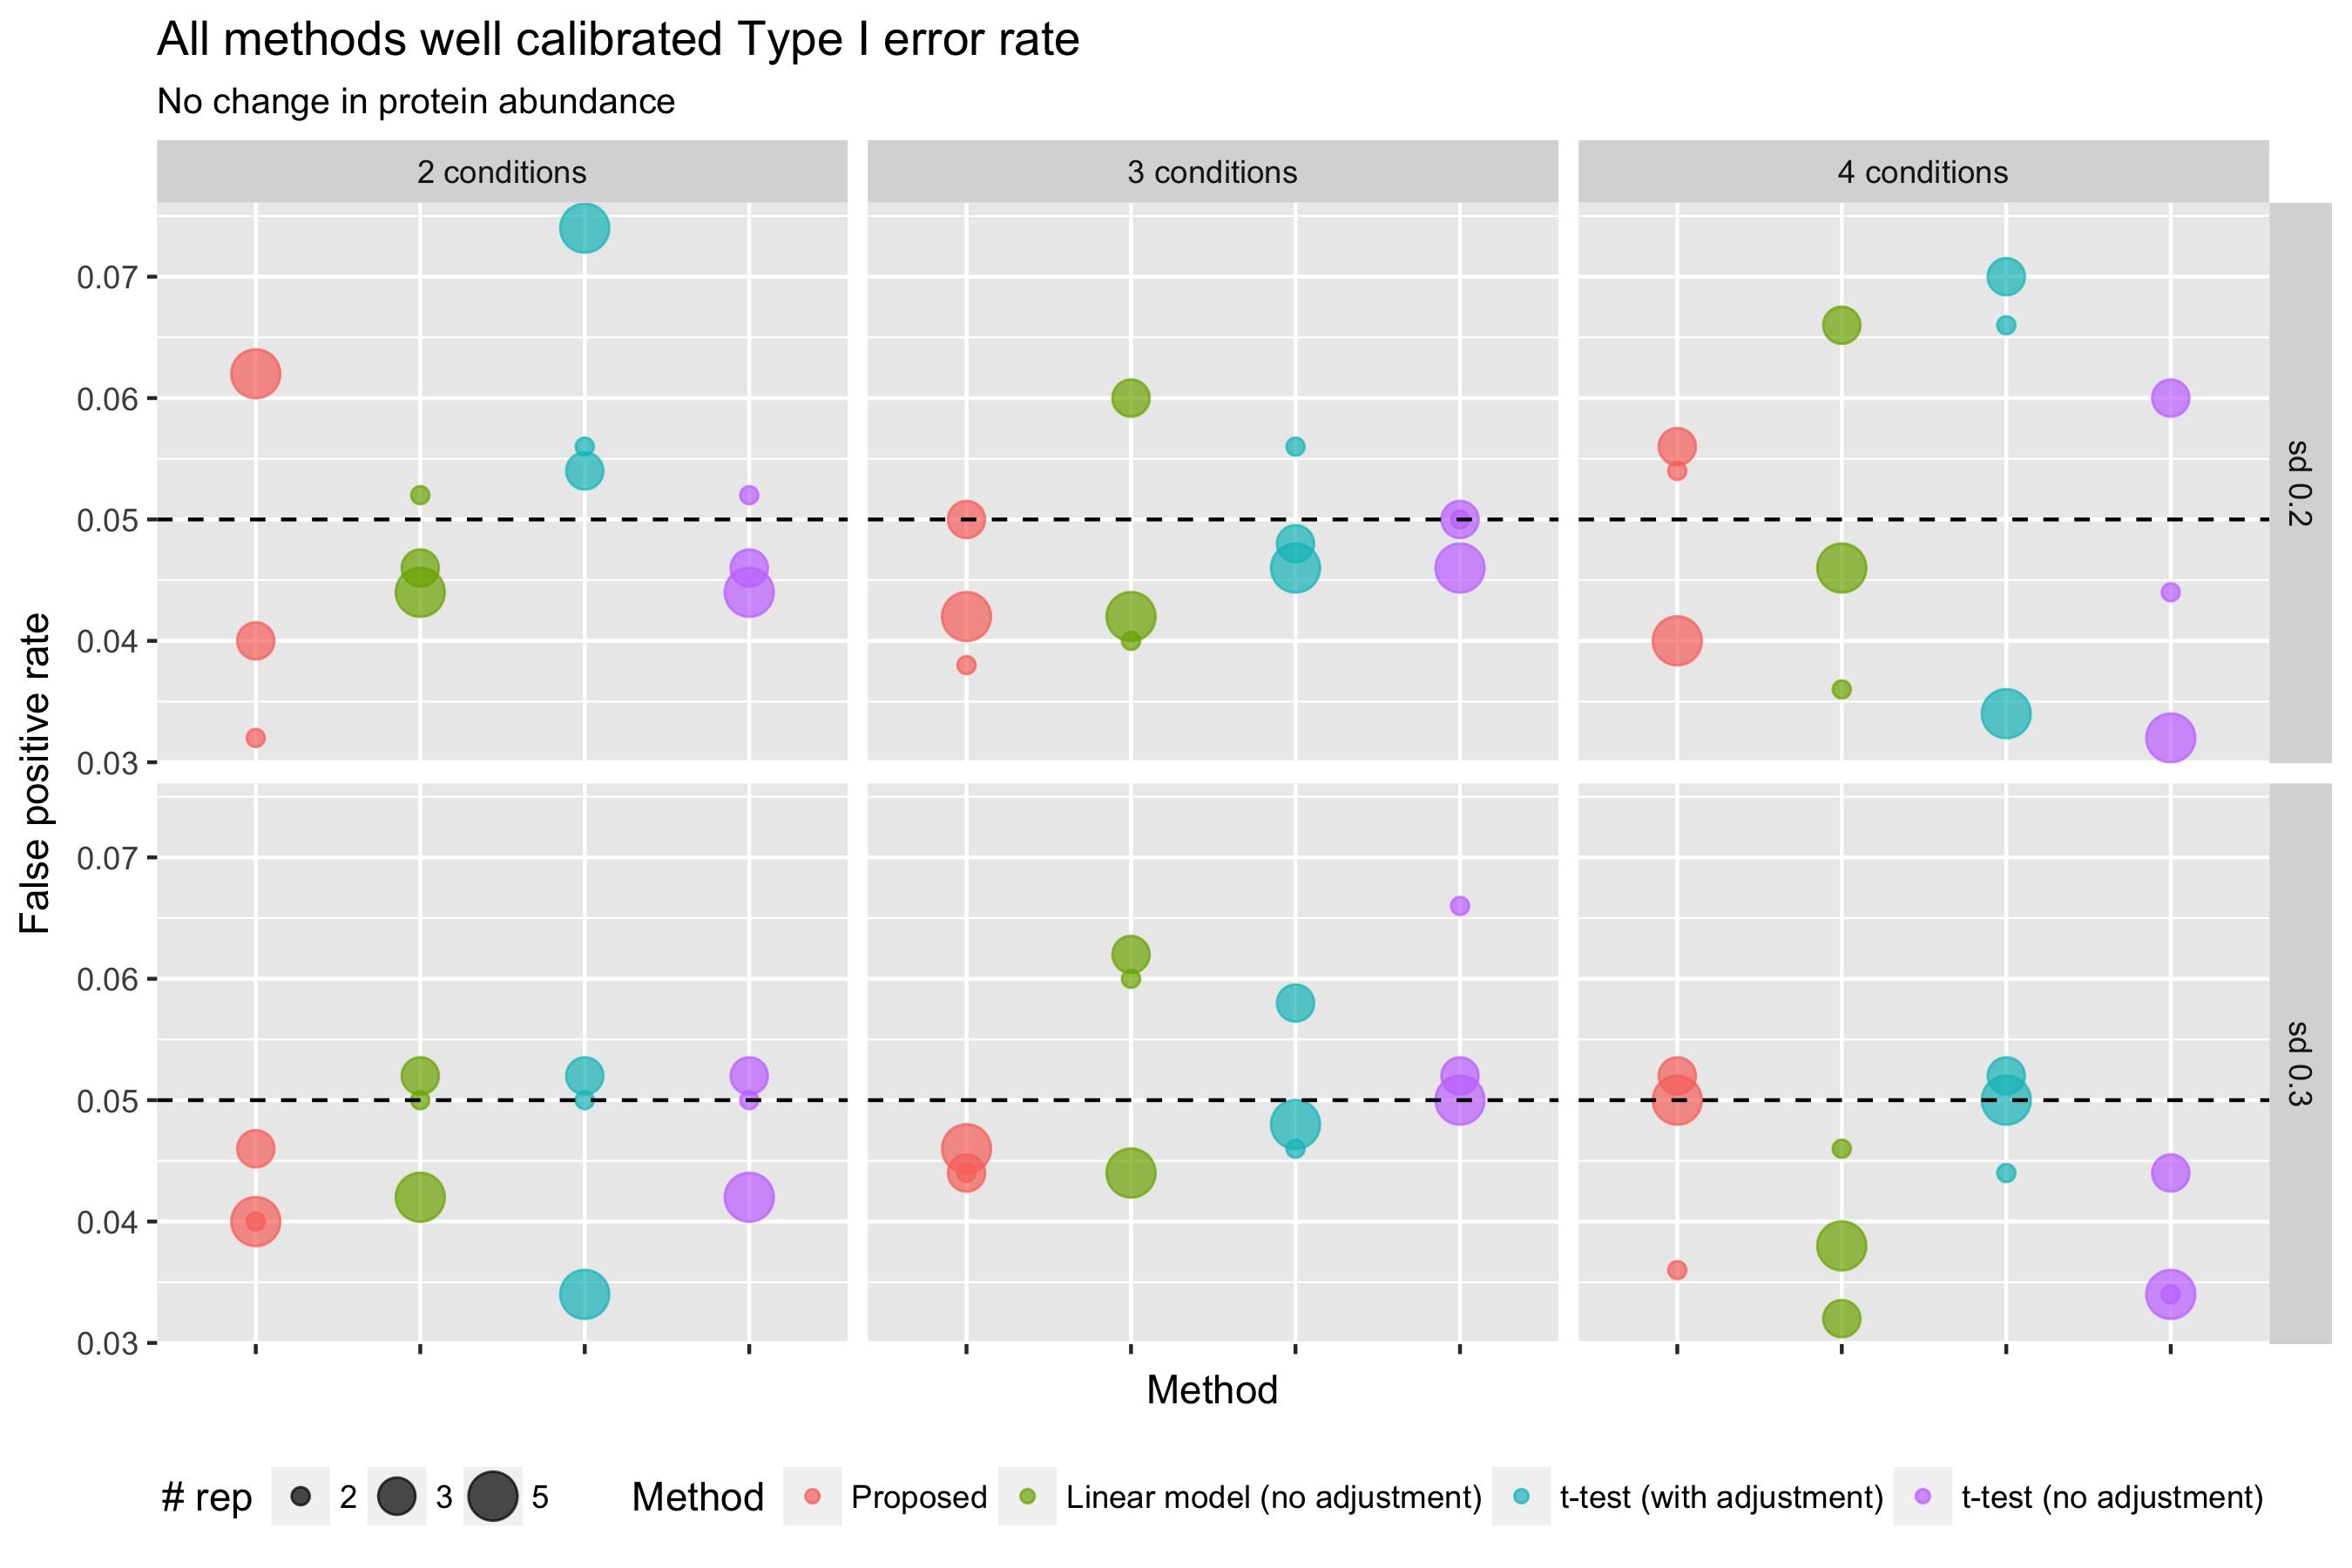
\includegraphics[width=.85\textwidth]{sim/protnull_fpr}\\
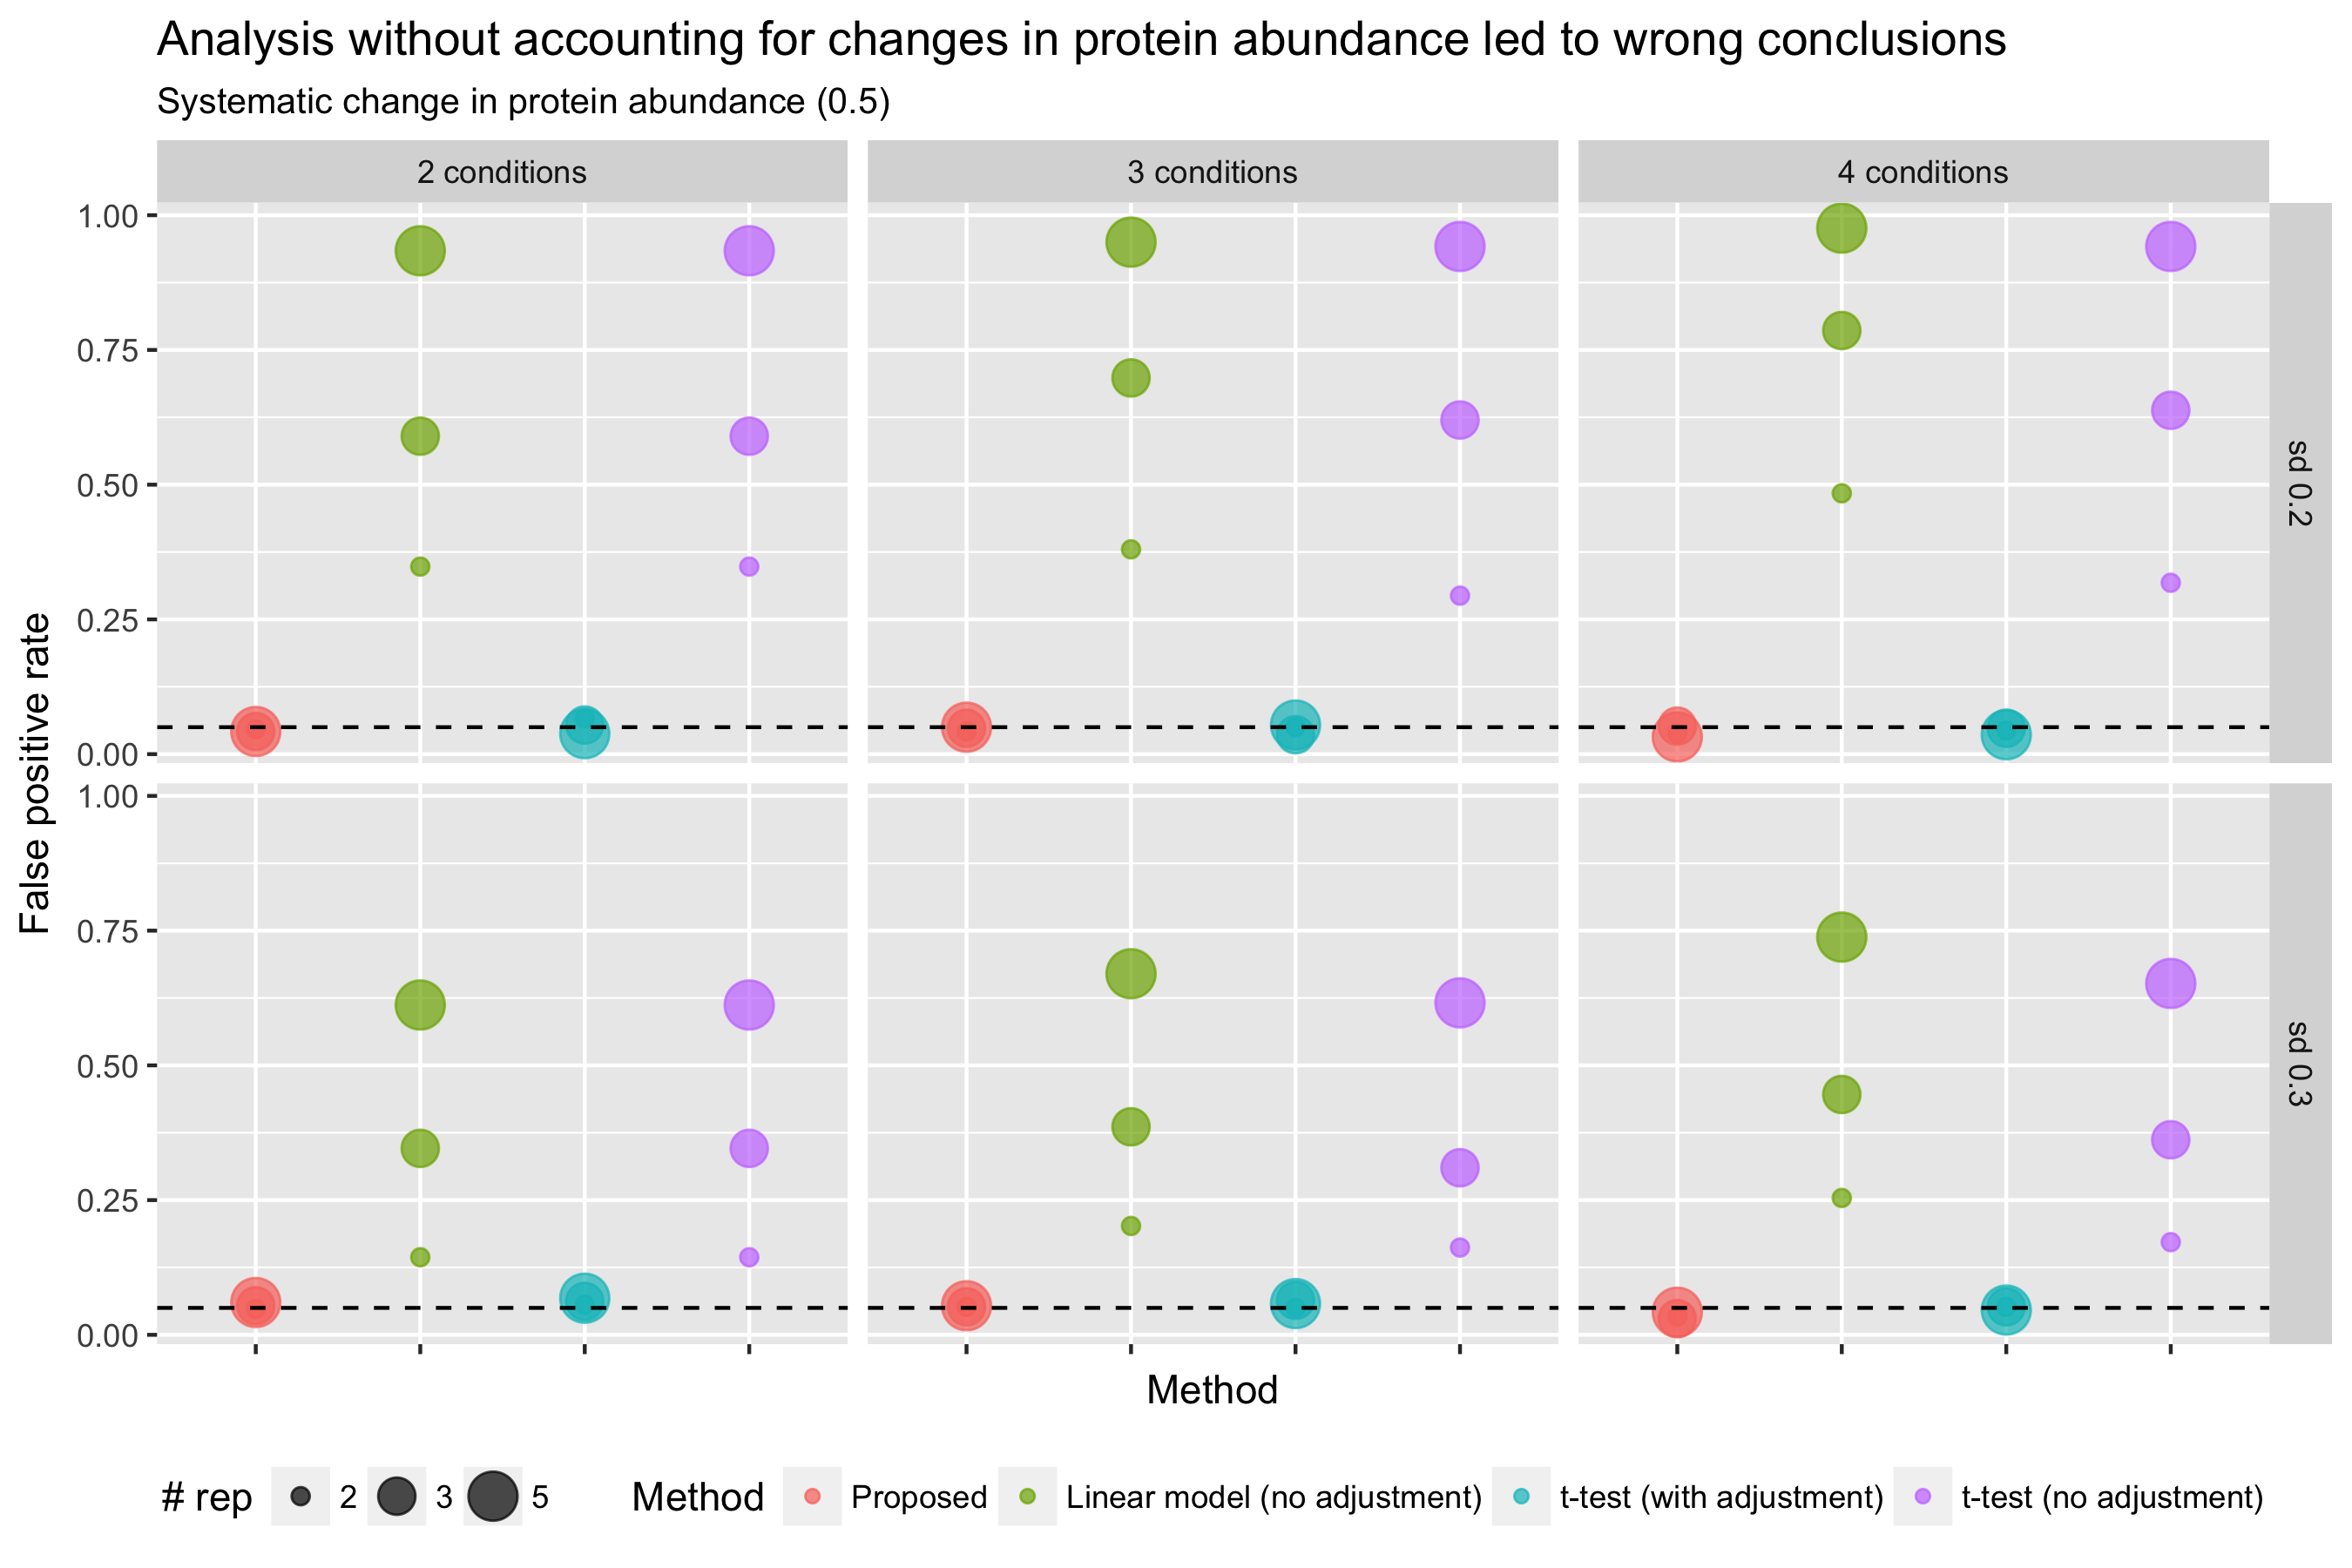
\includegraphics[width=.85\textwidth]{sim/protalt_fpr}
\caption{All the considered methods well calibrated the Type I error rate when there was no change in protein abundance (upper plot). When the
changes in PTM abundance were entirely due to changes in protein abundance across conditions (bottom plot), analysis without accounting for the protein-level changes resulted in off-target, high false positive rates. \label{fig:prot_fpr}}
\end{figure}

\begin{figure}[h!]
\centering
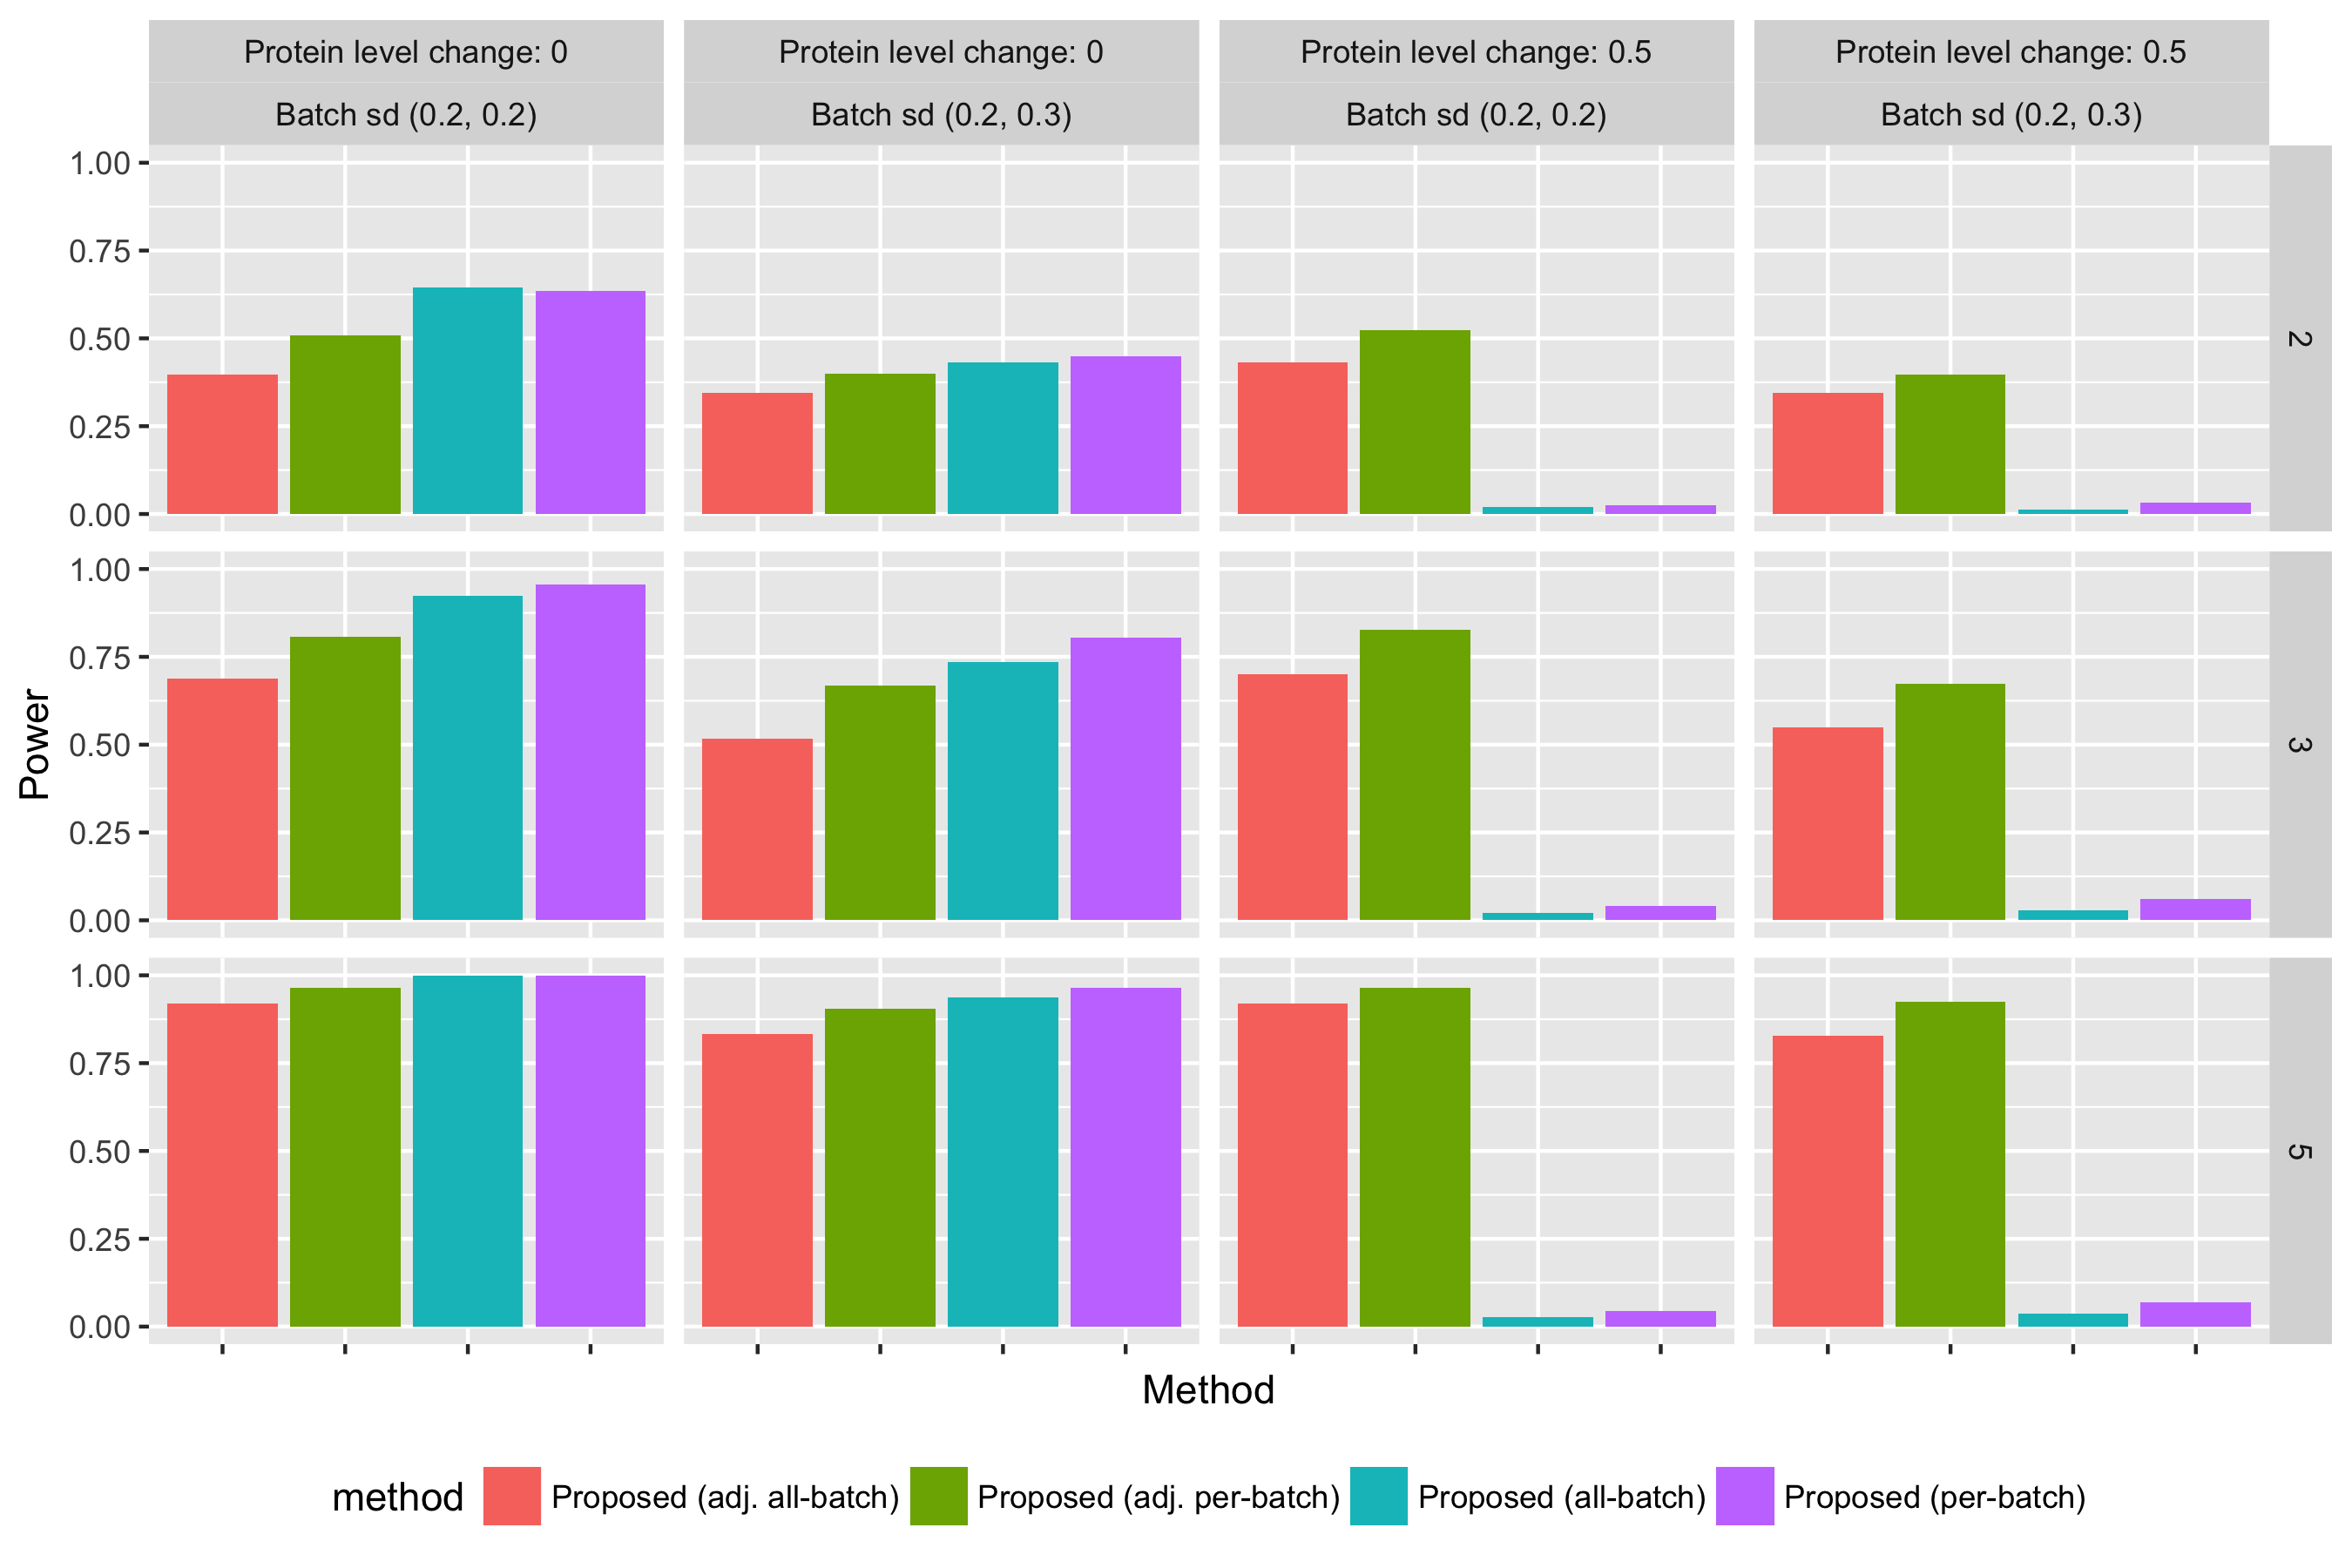
\includegraphics[width=\textwidth]{sim/prot_pwr}
%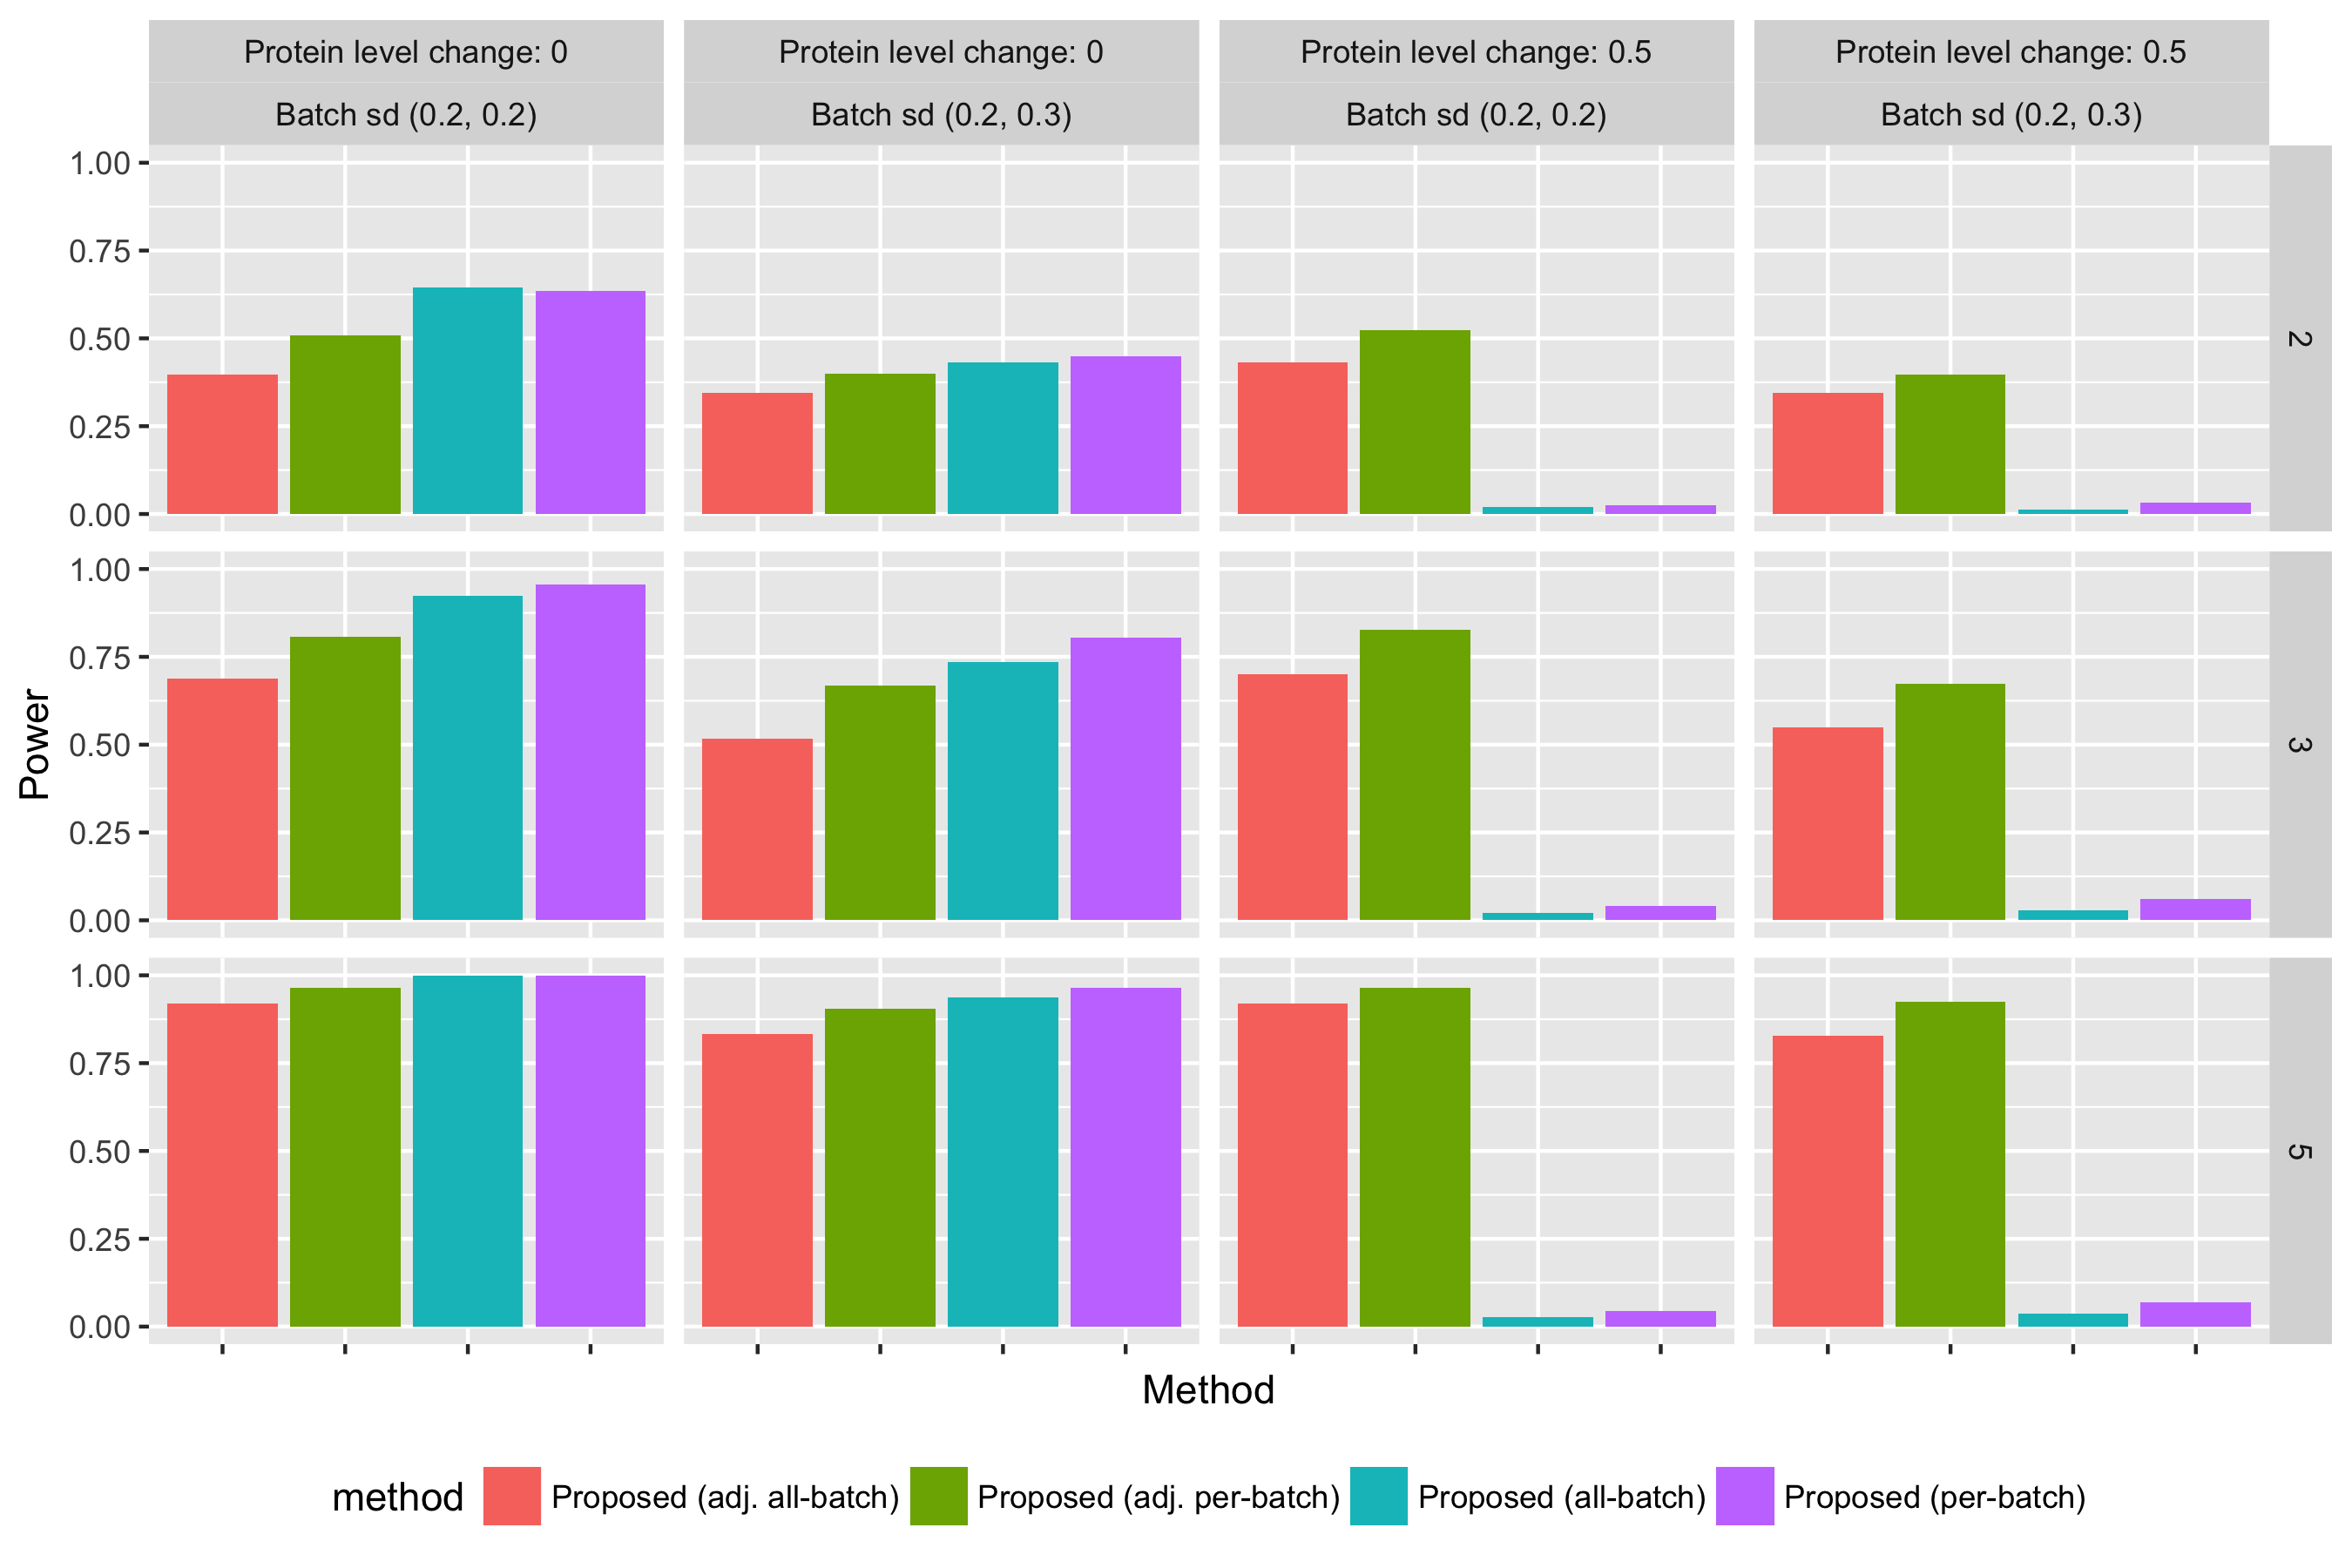
\includegraphics[width=.85\textwidth]{sim/prot_pwr}
\caption{In comparison between the proposed approach and $t$-test with protein-level adjustment, the proposed approach improved power with small sample sizes. Two-sample $t$-test only used data within the groups of interest while ignoring the rest the of data. Consequently, it gave similar performance across cases with different number of conditions. In contrast, the proposed approach leveraged all available information, which resulted in improved power with increased number of conditions.\todo{how about protein abundance change?} \todo{this conclusion seems that overfitting.. more number of conditions increase the power.. Then how about limma?} \todo{how to calculate estimated sigma for 4 conditions and t-test?} \label{fig:prot_pwr}}
\end{figure}

\begin{figure}[h!]
\centering
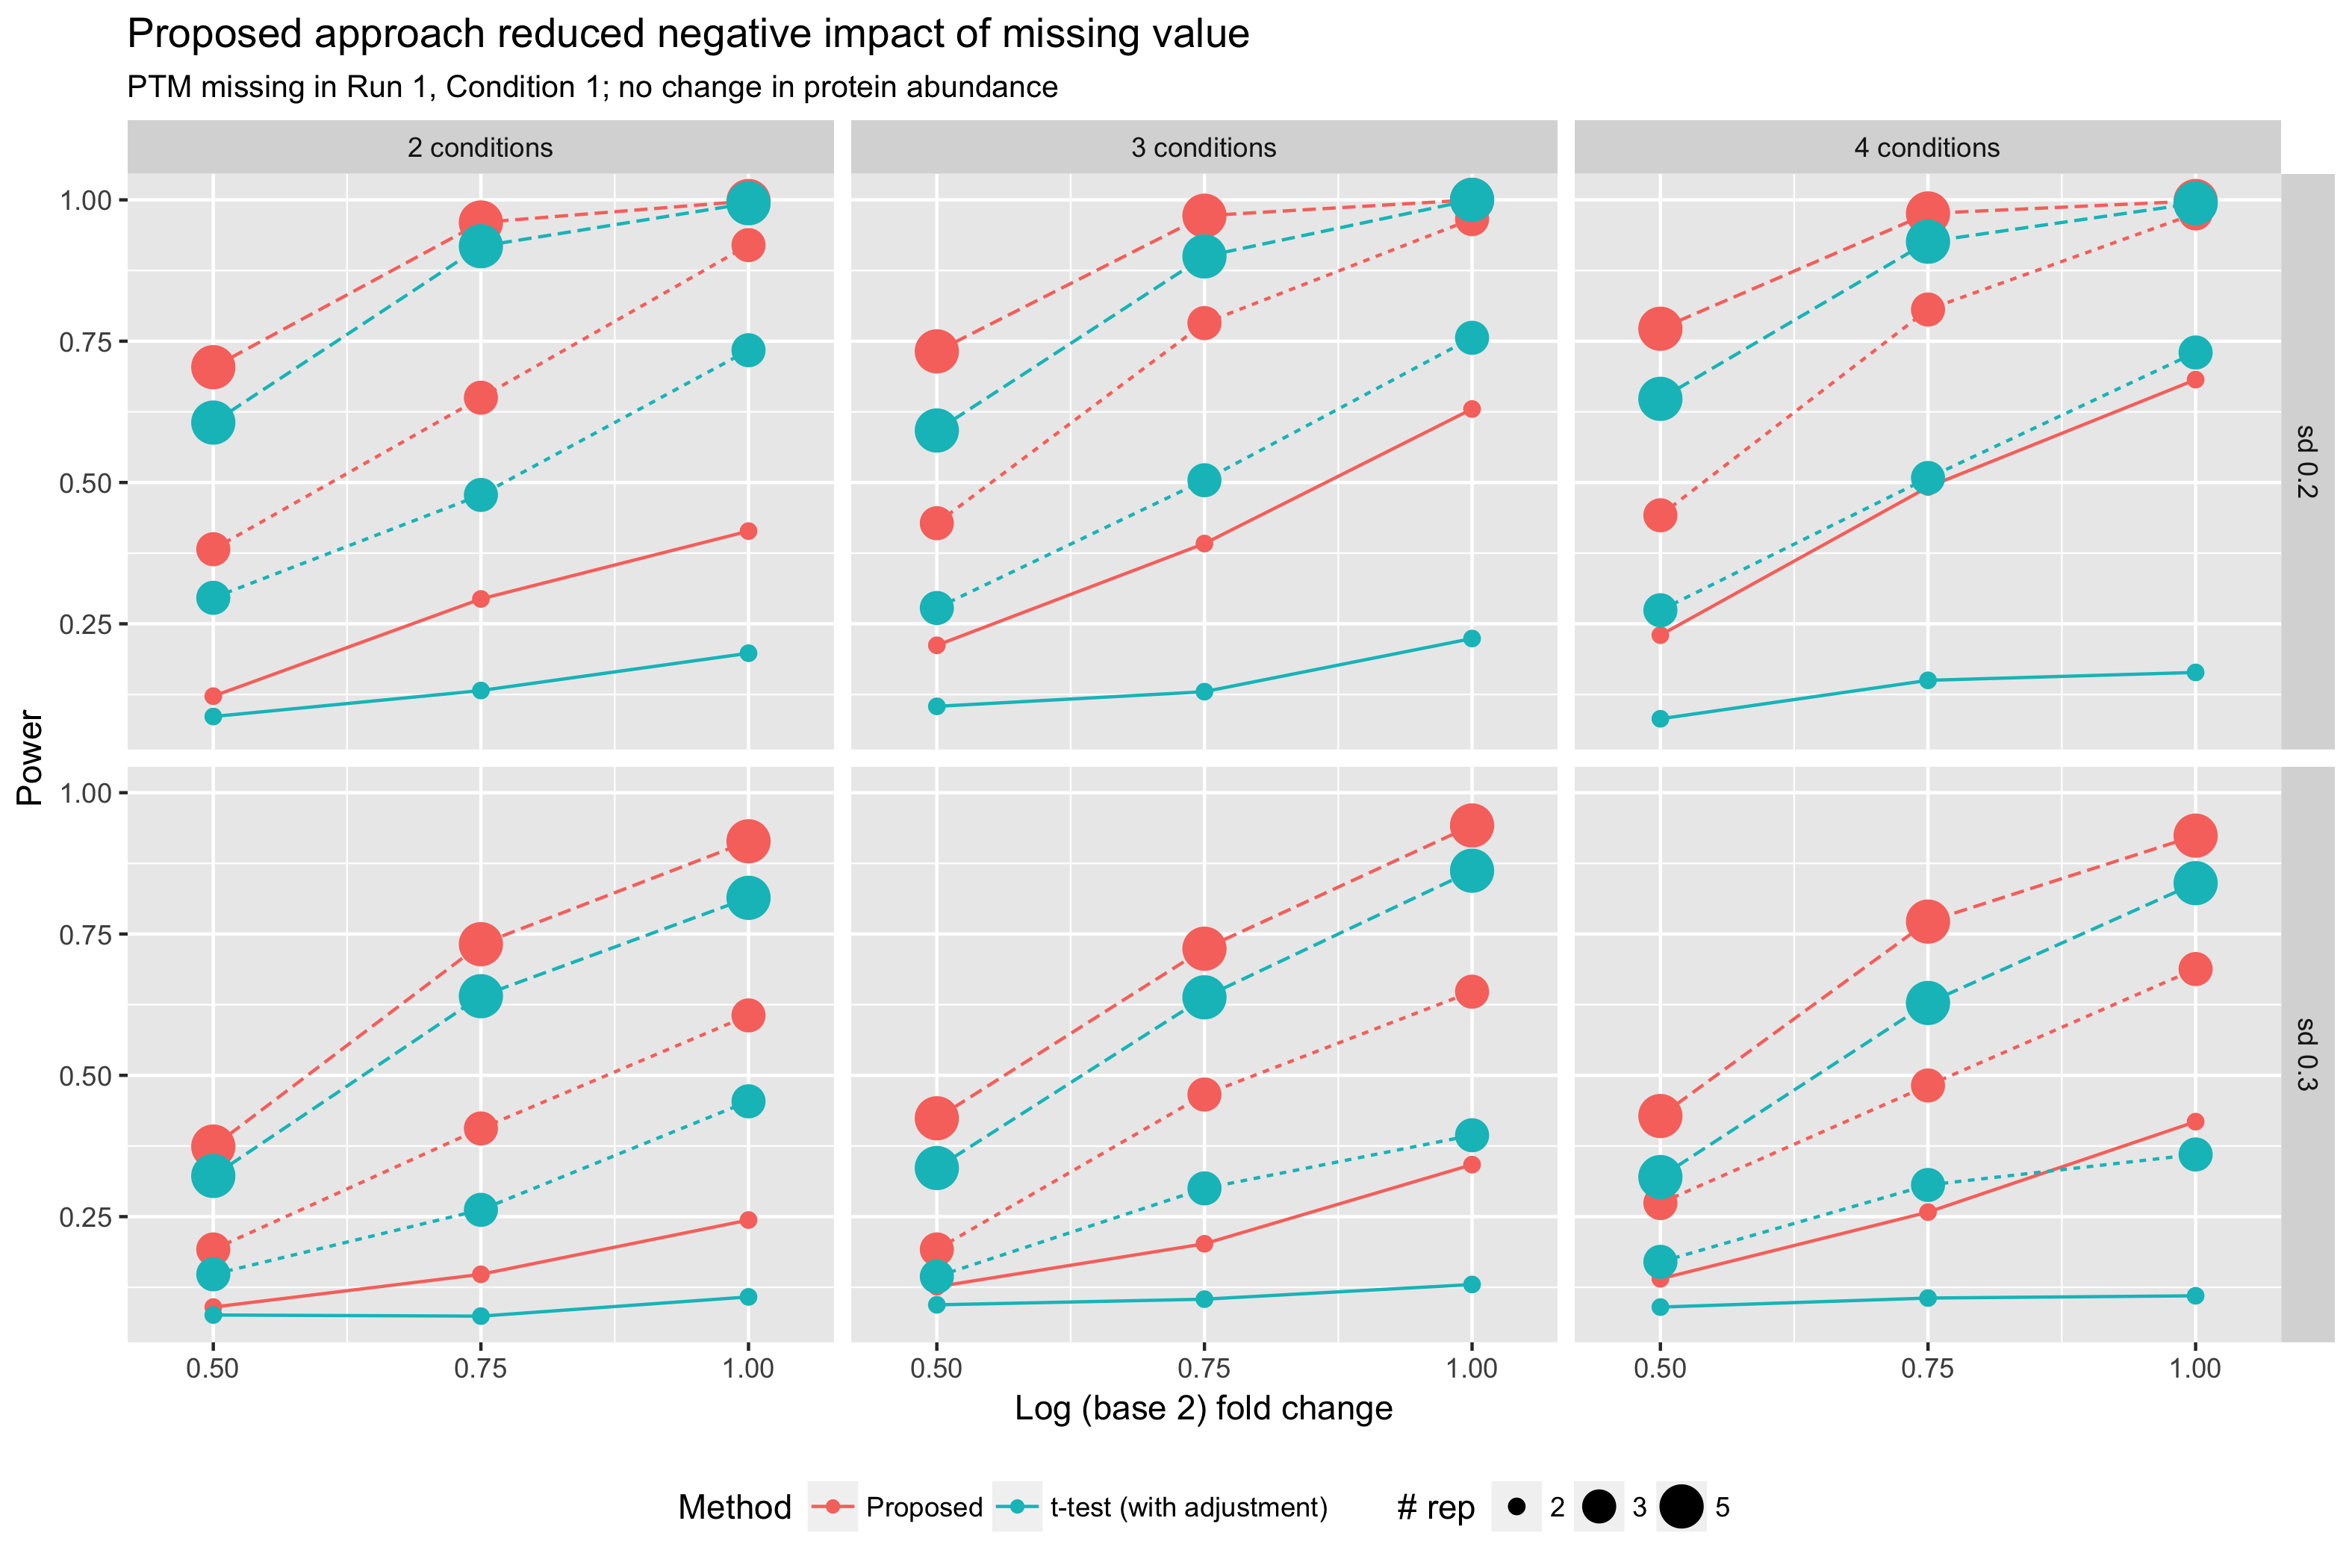
\includegraphics[width=\textwidth]{sim/protm1_pwr}
%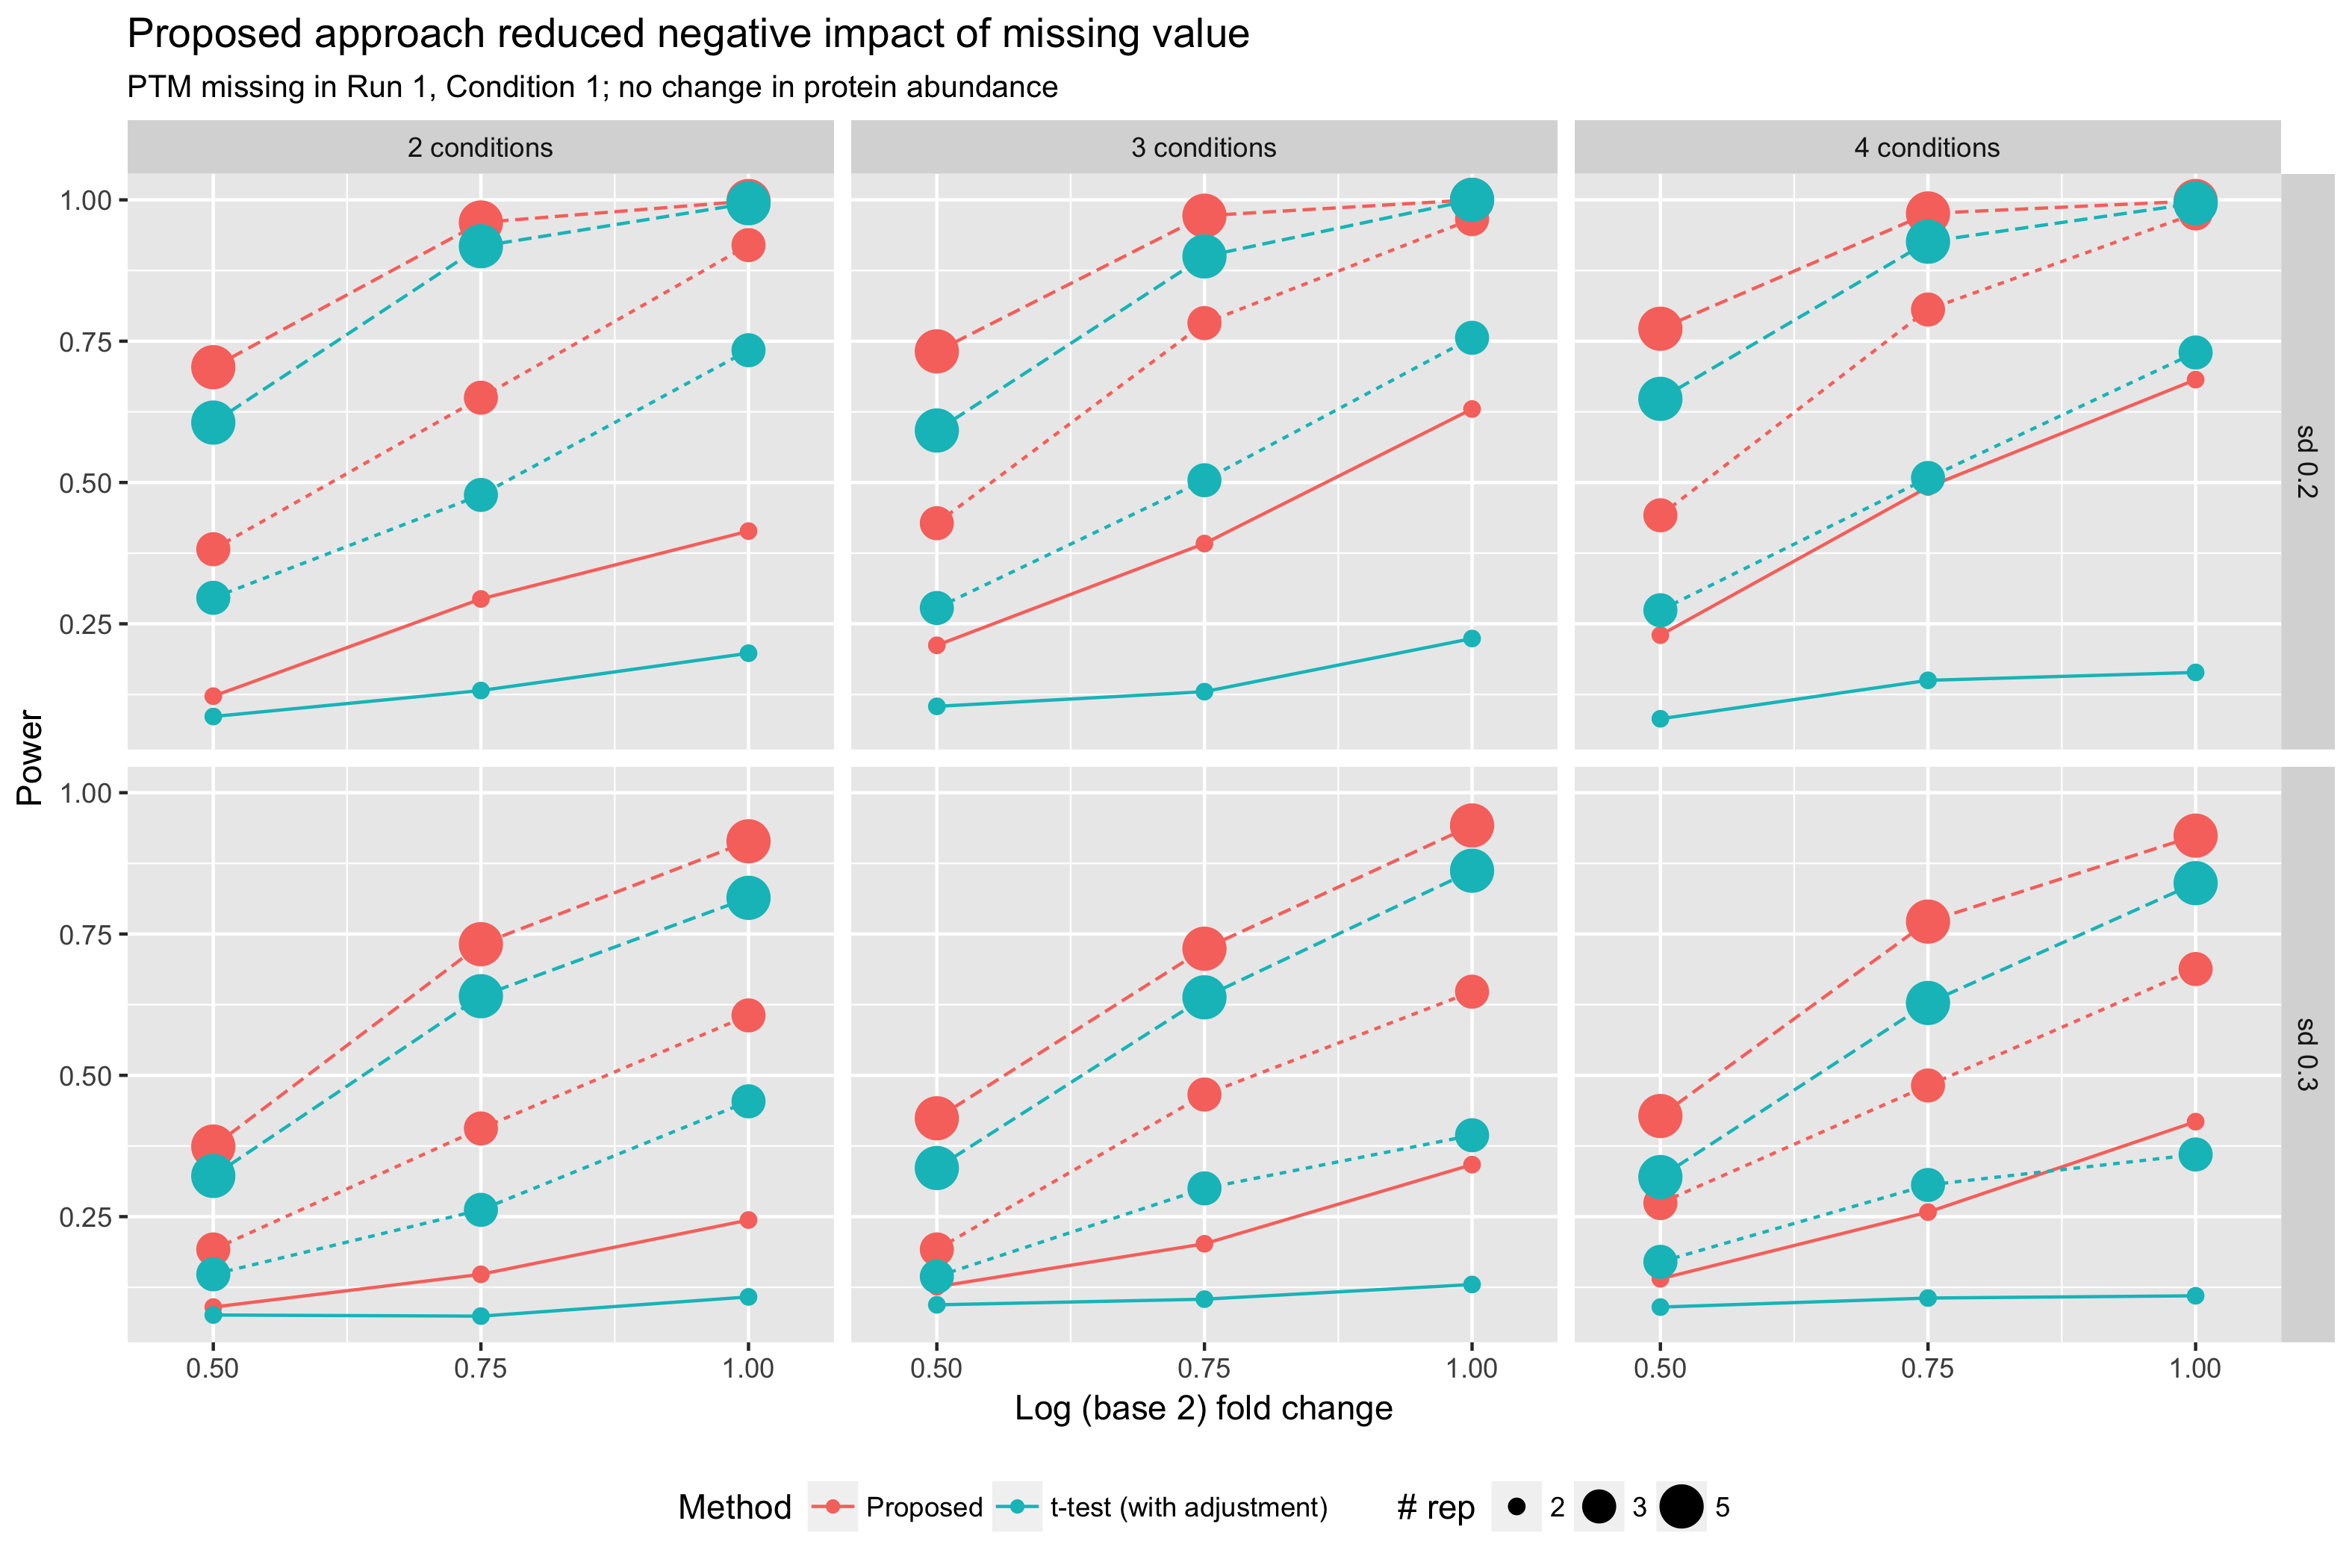
\includegraphics[width=.85\textwidth]{sim/protm1_pwr}
\caption{The advantage by using the proposed approach over two-sample $t$-test became more profound in the presence of missing value. In cases with small sample sizes, performance by the $t$-test decreased dramatically with one missing value. As a specific example, the statistical power by using the $t$-test with two replicates was below $0.25$, and increasing the fold change to $2$ did not effectively reduce the negative impact. \label{fig:protm1_pwr}}
\end{figure}


%%%%%%%%%%%%%%%%%%%%%%%%%%%%%%%%%%%%%%%%%%%%%%%%%%%%%%%%%%%%%%%%
\subsubsection{Multiple sites per protein}

Expression levels of PTM sites are adjusted based on the abundance of their originating protein. Since the same reference is used for all sites, it introduces correlation among estimates and test statistics for those sites. This may cause issues in controlling false discovery rate (FDR).
We investigated the property by simulating data of two conditions and 1000 proteins with different numbers of PTM sites and comparing the results of the proposed approach and the linear model with no adjustment. 
%We investigated the property by simulating data of two conditions and 1000 proteins with different numbers of PTM sites. 
A fraction (50\%) of the 1000 proteins had no changes between conditions while systematic changes were simulated for the rest of the proteins. Multiple testing correction was performed using the Benjamini and Hochberg's method. 
Performances of the considered approaches were assessed by their actual FDR, calculated as the fraction of proteins with adjusted $p$-values $<0.05$ among the proteins with true differences. The results are summarized in \sfigref{fig:prot_fdr}.
%Performances of the considered approaches were assessed by their power and FDR. The power was calculated as the fraction of proteins with adjusted $p$-values $<0.05$ among those proteins with true differences between conditions, while the FDR was calculated as the fraction of proteins with adjusted $p$-values $<0.05$ among the proteins with true differences. The results are summarized in \sfigref{fig:prot_fdr}.

\todo{should address number of replicates, standard deviations, missing data?, same as one site per protein.}
\todo{not strong evidence. need to revisit this section.}

\begin{figure}[h!]
\centering
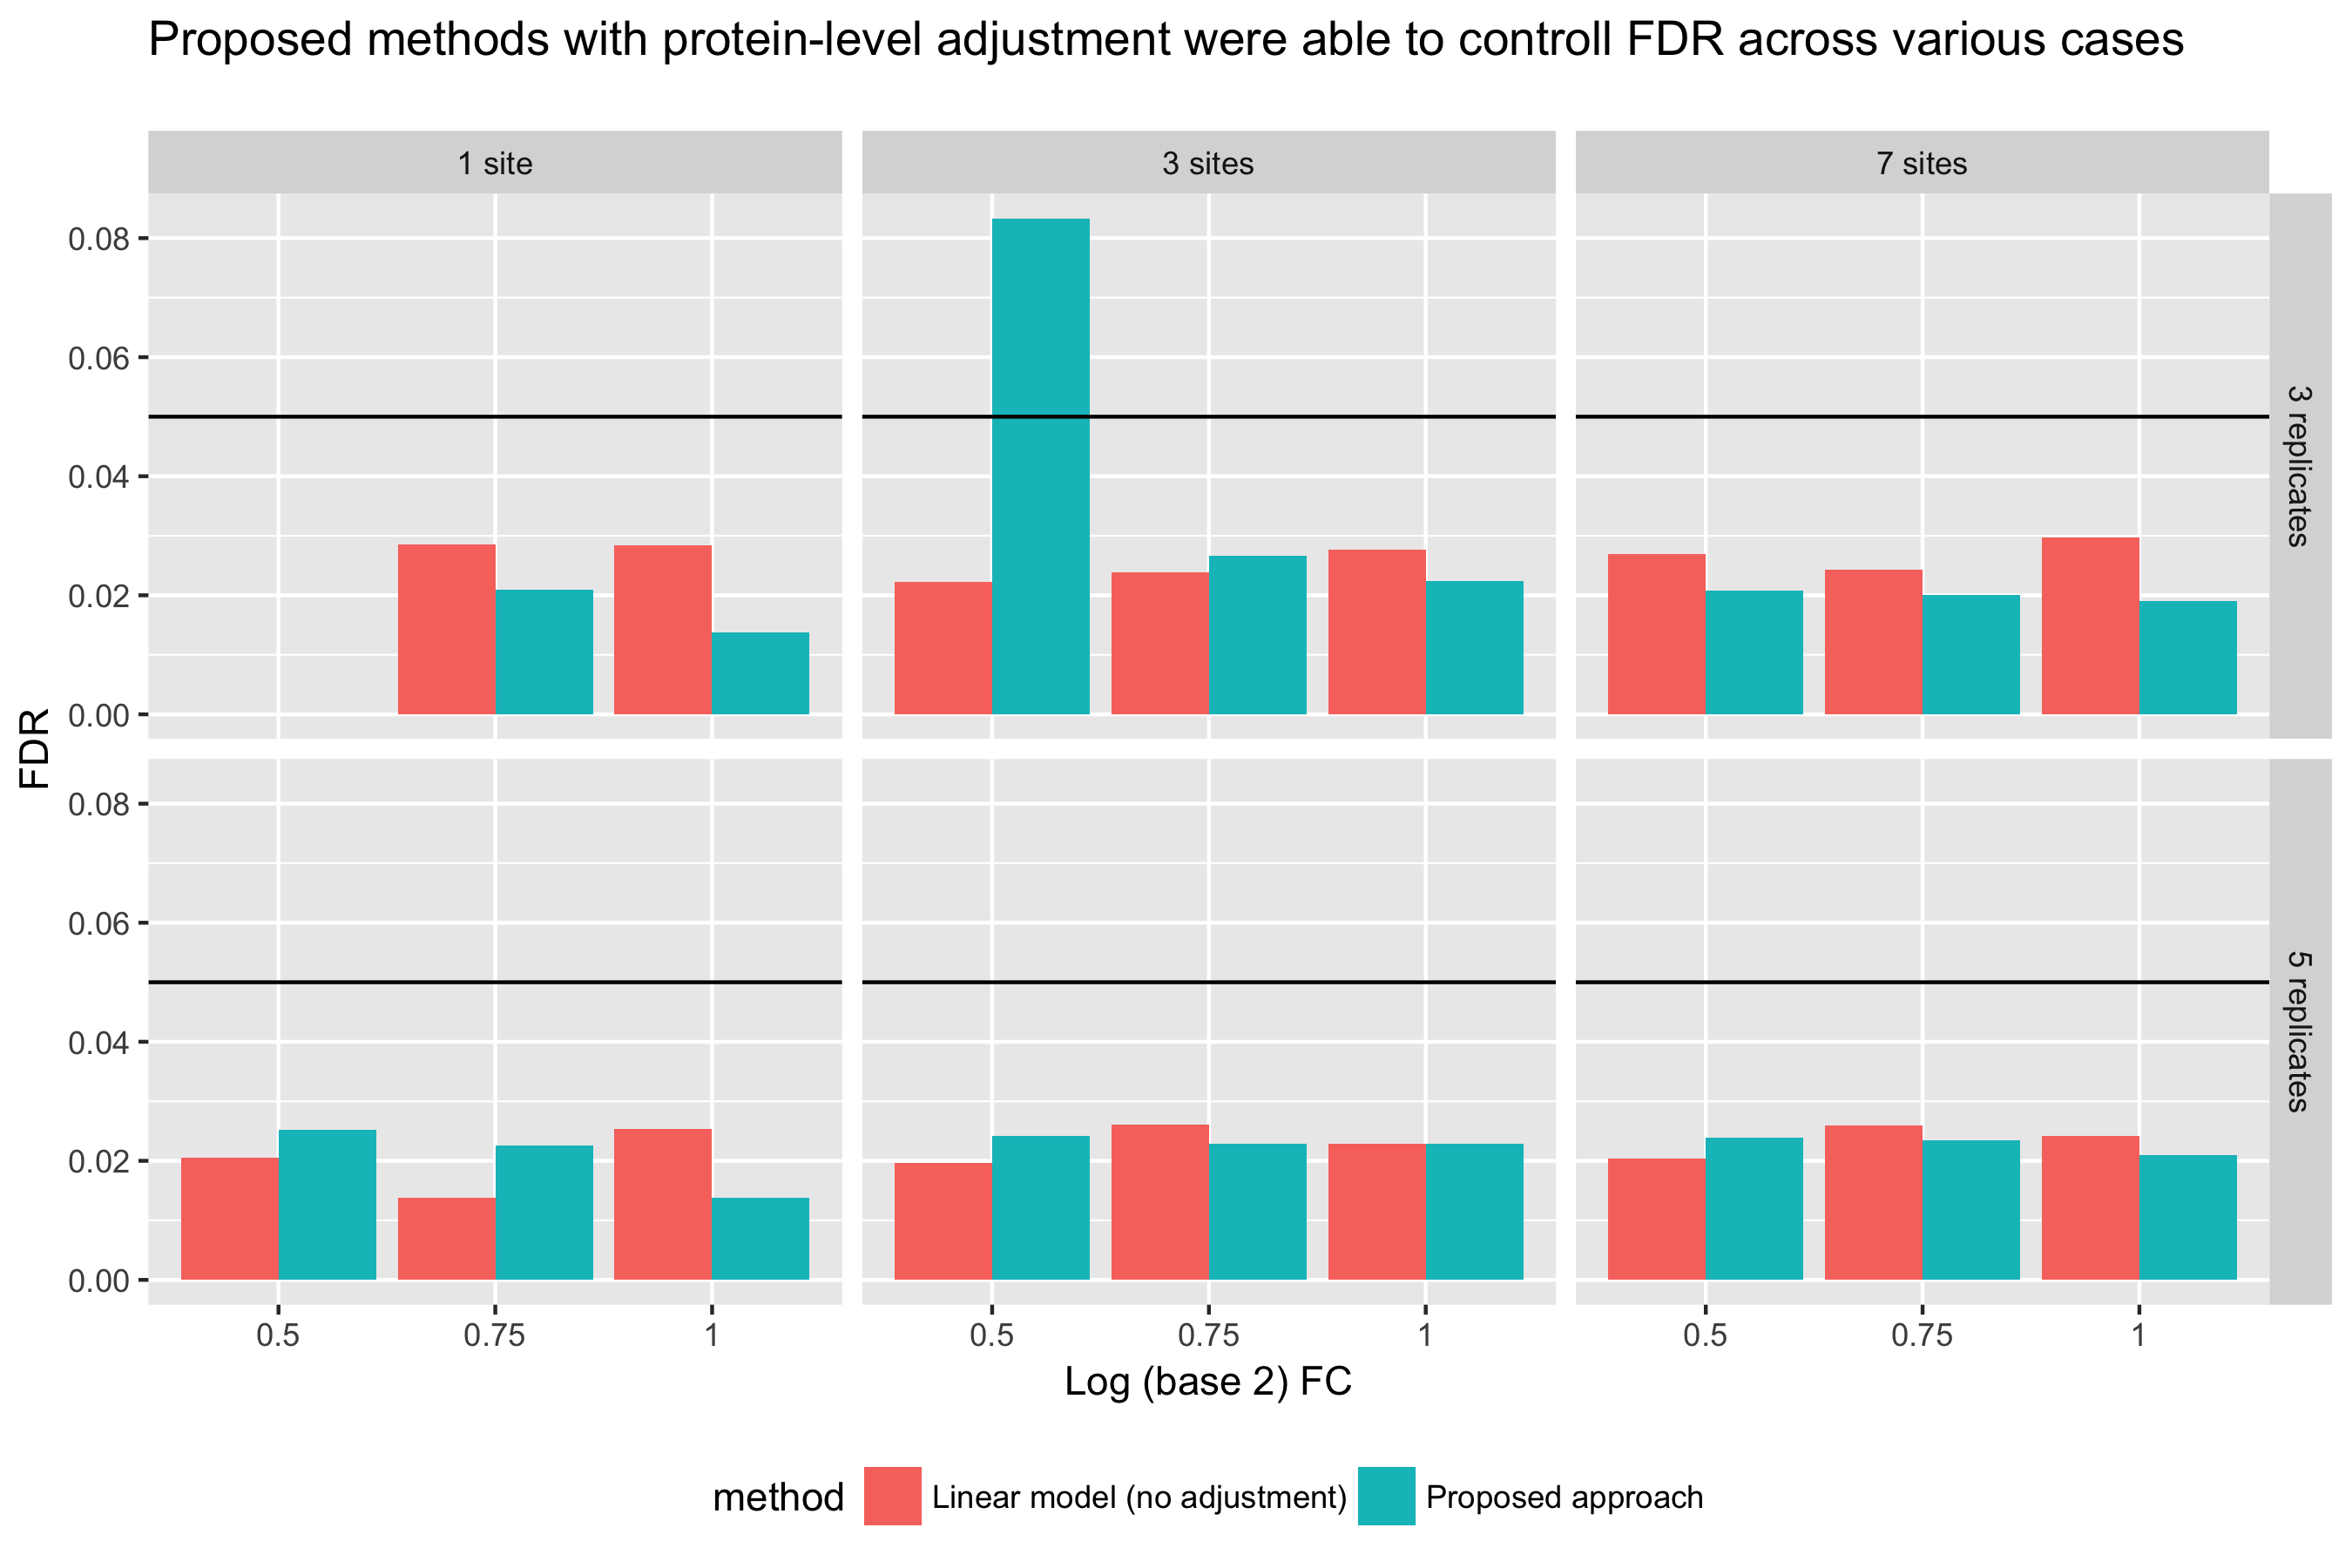
\includegraphics[width=.85\textwidth]{sim/prot_fdr}
\caption{Correlation between test statistics across sites due to protein-level adjustment did not affect the expected level of FDR under the considered scenarios. The Benjamini-Hochberg procedure was used to control the FDR.\todo{make same color for each method} \label{fig:prot_fdr}}
\end{figure}


\clearpage
%%%%%%%%%%%%%%%%%%%%%%%%%%%%%%%%%%%%%%%%%%%%%%%%%%%%%%%%%%%%%%%%
\subsection{Batch effects}

We evaluated the statistical properties of the proposed approach under batch effects, in comparison to the two-sample $t$-test (\secref{sec:ttest}). While the $t$-test is not directly applicable to a problem with batches of data, several \textit{ad-hoc} approaches may be used. Two commonly used approaches are a) $t$-test (no batch): ignoring batch effects when applying $t$-test, and b) $t$-test (most significant batch): applying $t$-test in each batch and drawing conclusions based on the most significant batch. Although simple, these \textit{ad-hoc} methods lack statistical justification. We characterized their statistical properties under various forms of batch effects. In this part of the simulation, two batches of data were generated, with the following forms of batch effects: difference in signal intensities across batches, difference in variability across batches, and interaction effect between batch and condition (i.e., change between condition affected by batch). The following interaction scenarios were considered in the simulation: a) no interaction between condition and batch, i.e., same change across conditions in both batches, b) positive interaction as $25$\% greater change in the batch of higher level, and c) negative interaction as $25$\% lower change in the batch of higher level. Below are the parameters used in the simulation: 
\begin{itemize}
\item Mean of log-intensity: $25$
\item Increased intensity level of Batch 2 versus Batch 1: $0$, $1$, $2$
\item Standard deviations of log-intensity: $0.2$ in Batch 1 and $0.3$ in Batch 2
\item Difference between conditions in Batch 1: $0.5$, $0.75$, $1$
\item Number of replicates: $2$, $3$, $5$
\item Number of conditions: $2$, $3$, $4$
\item Number of realizations: $500$
\end{itemize}
The following four approaches were compared: a) proposed approach, i.e., per-batch model, b) all-batch model, c) $t$-test (no batch), and d) $t$-test (most significant batch). The results are summarized from \sfigref{fig:synnull_est} to \sfigref{fig:synnull_pwr_5}, on the aspects of estimation error (\sfigref{fig:synnull_est}), false positive rate (\sfigref{fig:synnull_fpr}), and power (\sfigref{fig:synnull_pwr}, \sfigref{fig:synnull_pwr_5}). 

\begin{figure}[h!]
\centering
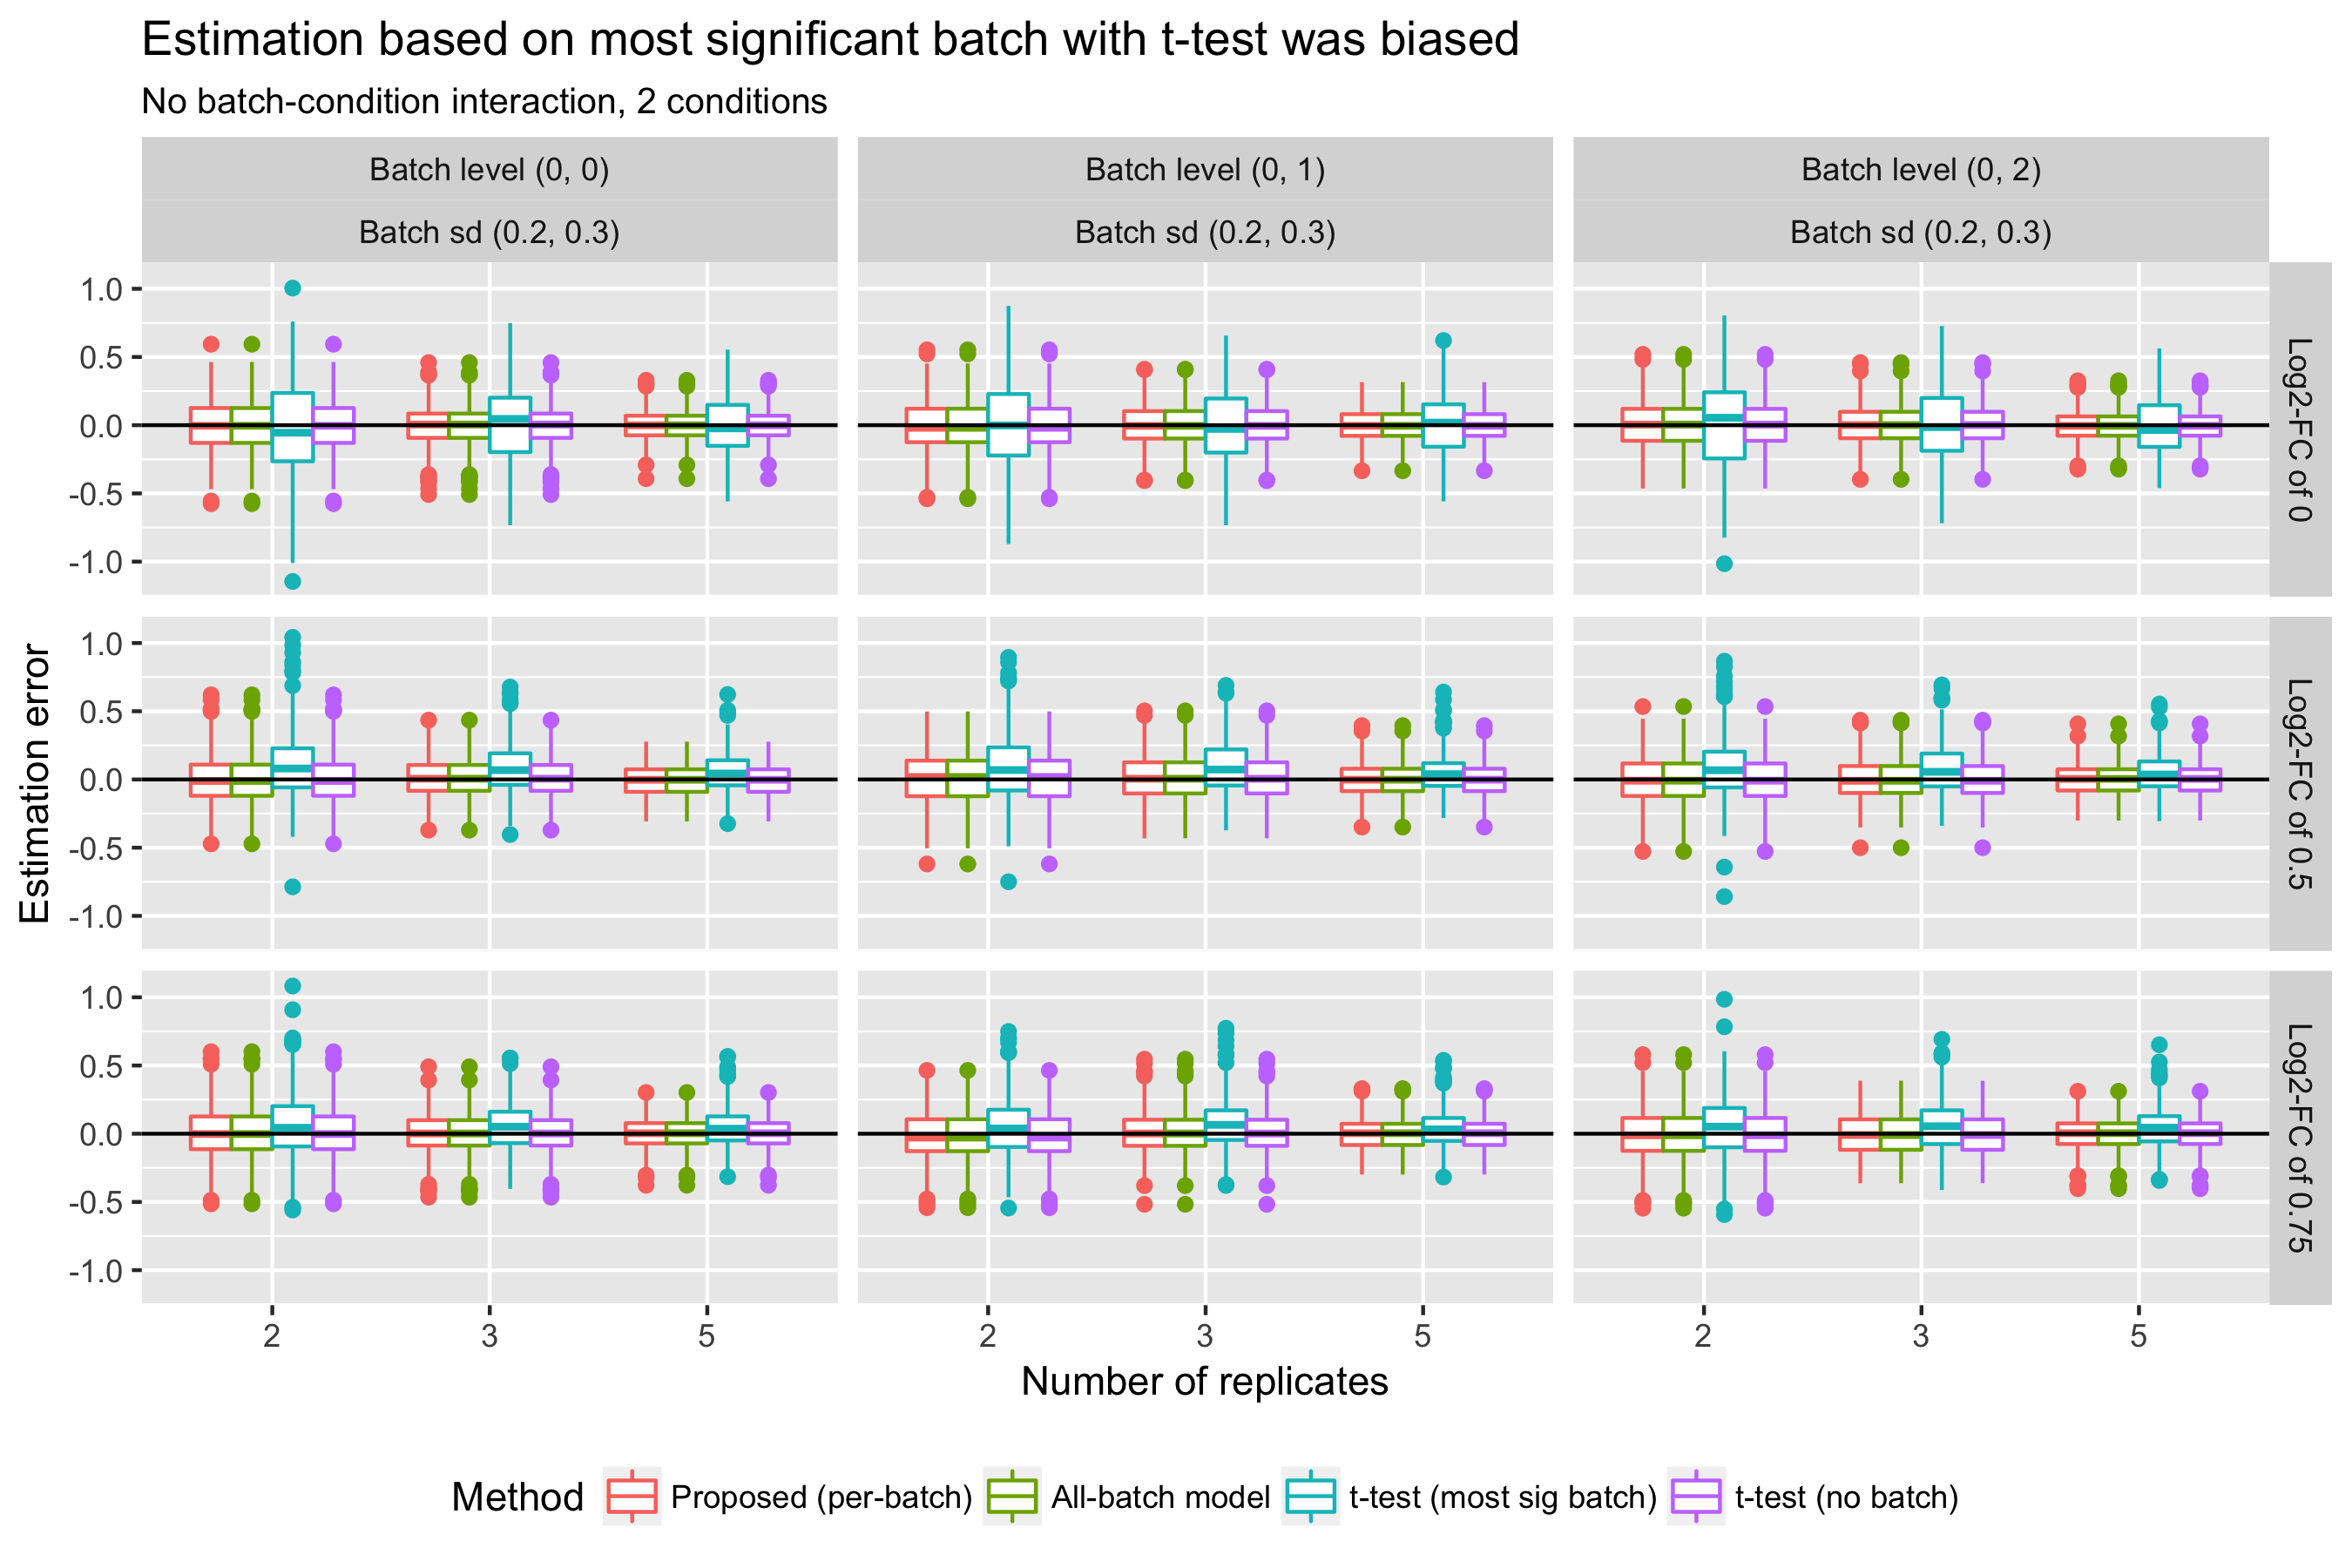
\includegraphics[width=.825\textwidth]{sim/synnull_est_2}
\caption{Estiamtion based on the most statistically significant batch with $t$-test was highly variable and frequently biased. The observation is consistent in all the simulated scenarios. \label{fig:synnull_est}}
\end{figure}

\begin{figure}[h!]
\centering
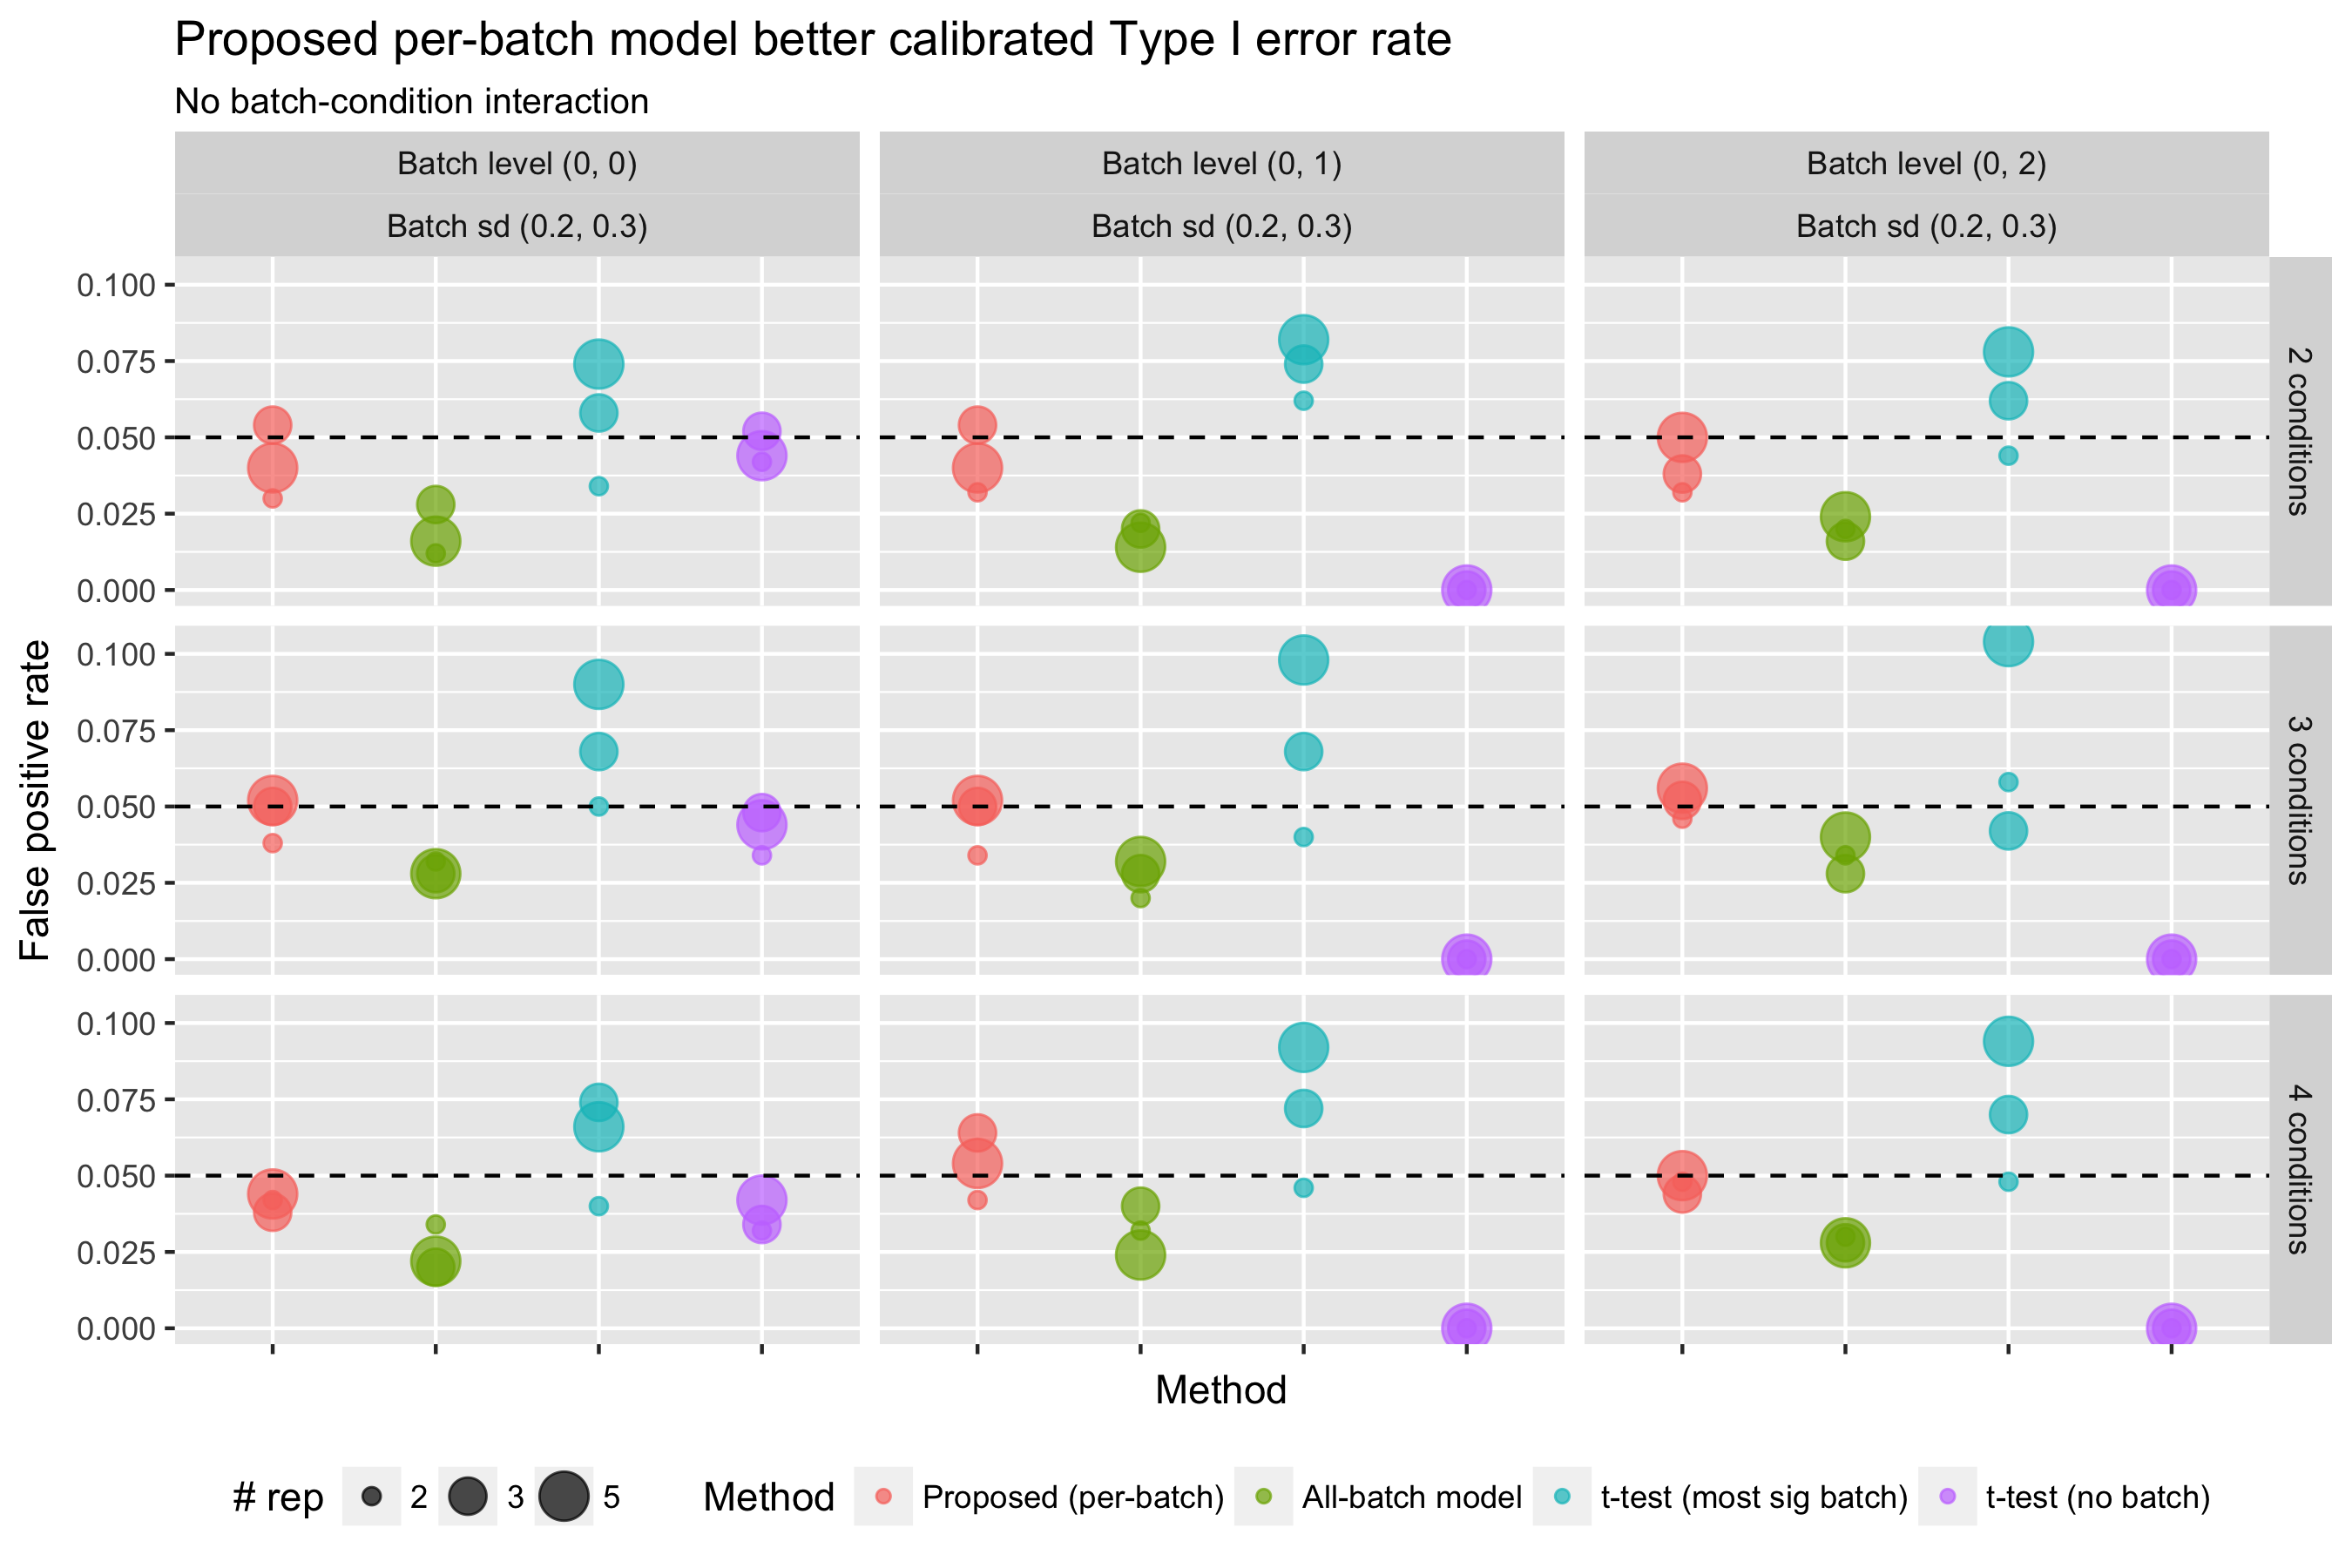
\includegraphics[width=.825\textwidth]{sim/synnull_fpr}
\caption{The proposed approach better calibrated Type I error rate. Similar results were observed in the cases with positive and negative batch-condition interactions. \label{fig:synnull_fpr}}
\end{figure}

\clearpage
\begin{figure}[h!]
\centering
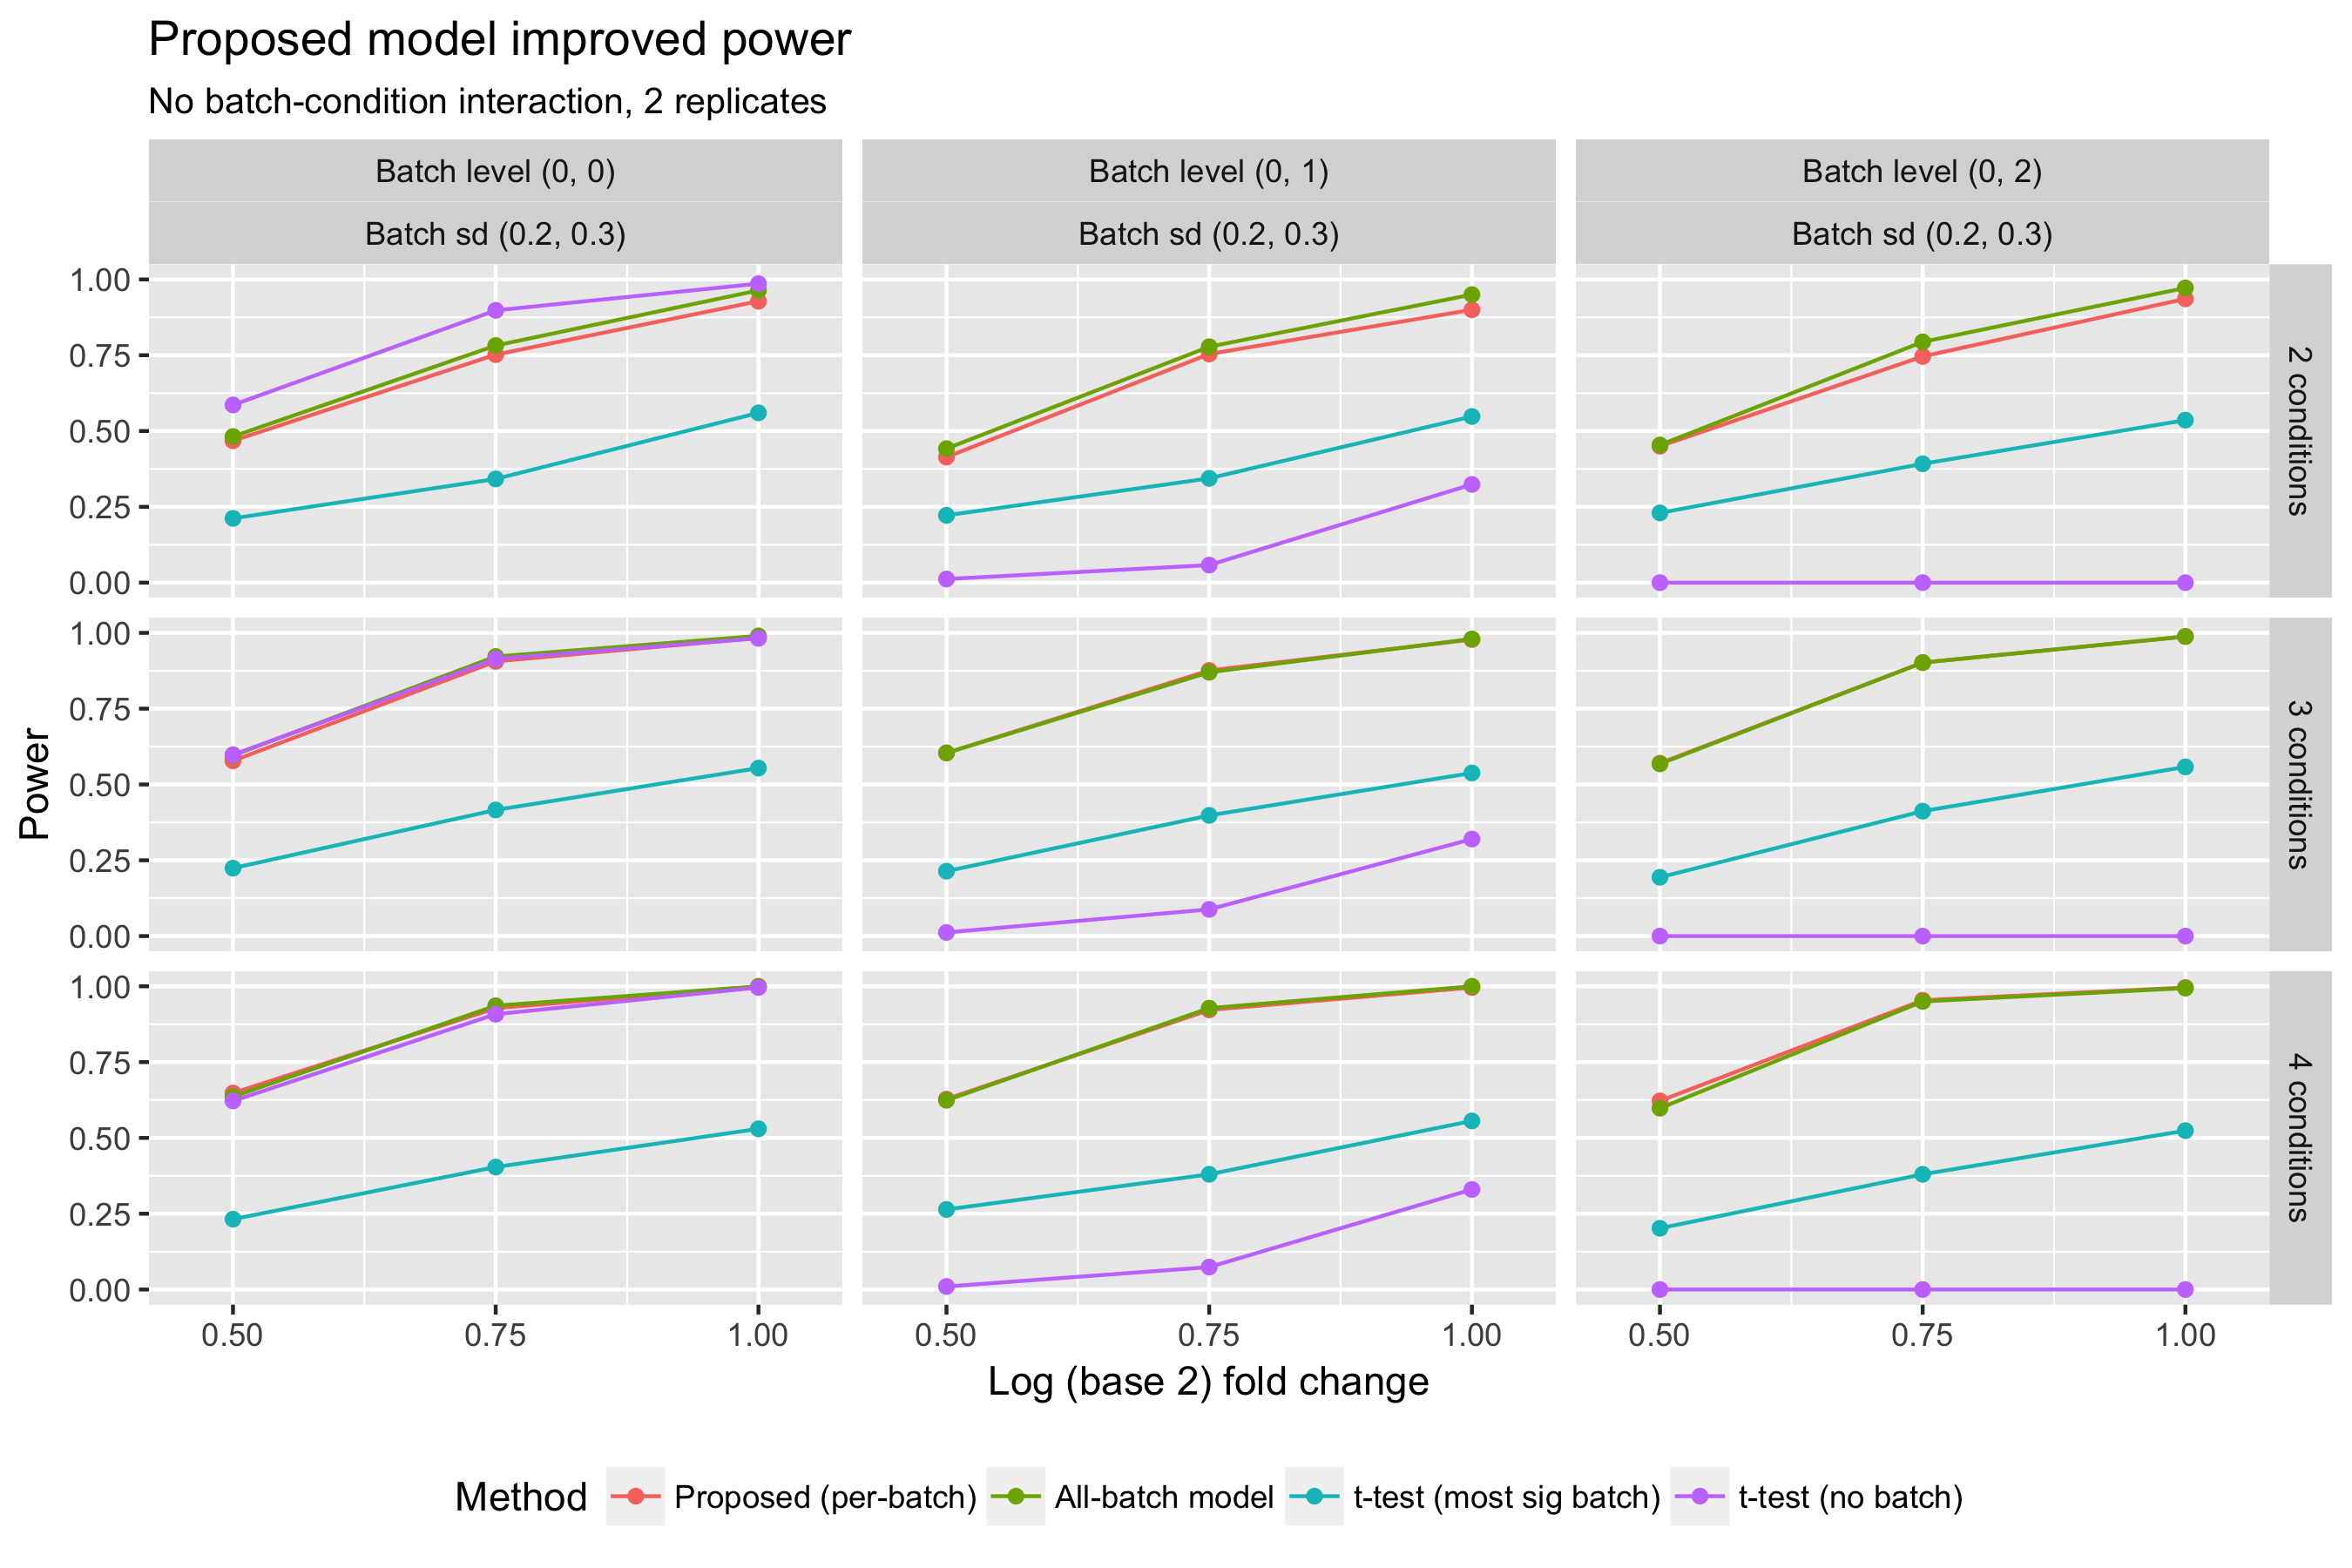
\includegraphics[width=.825\textwidth]{sim/synnull_pwr_2}\\
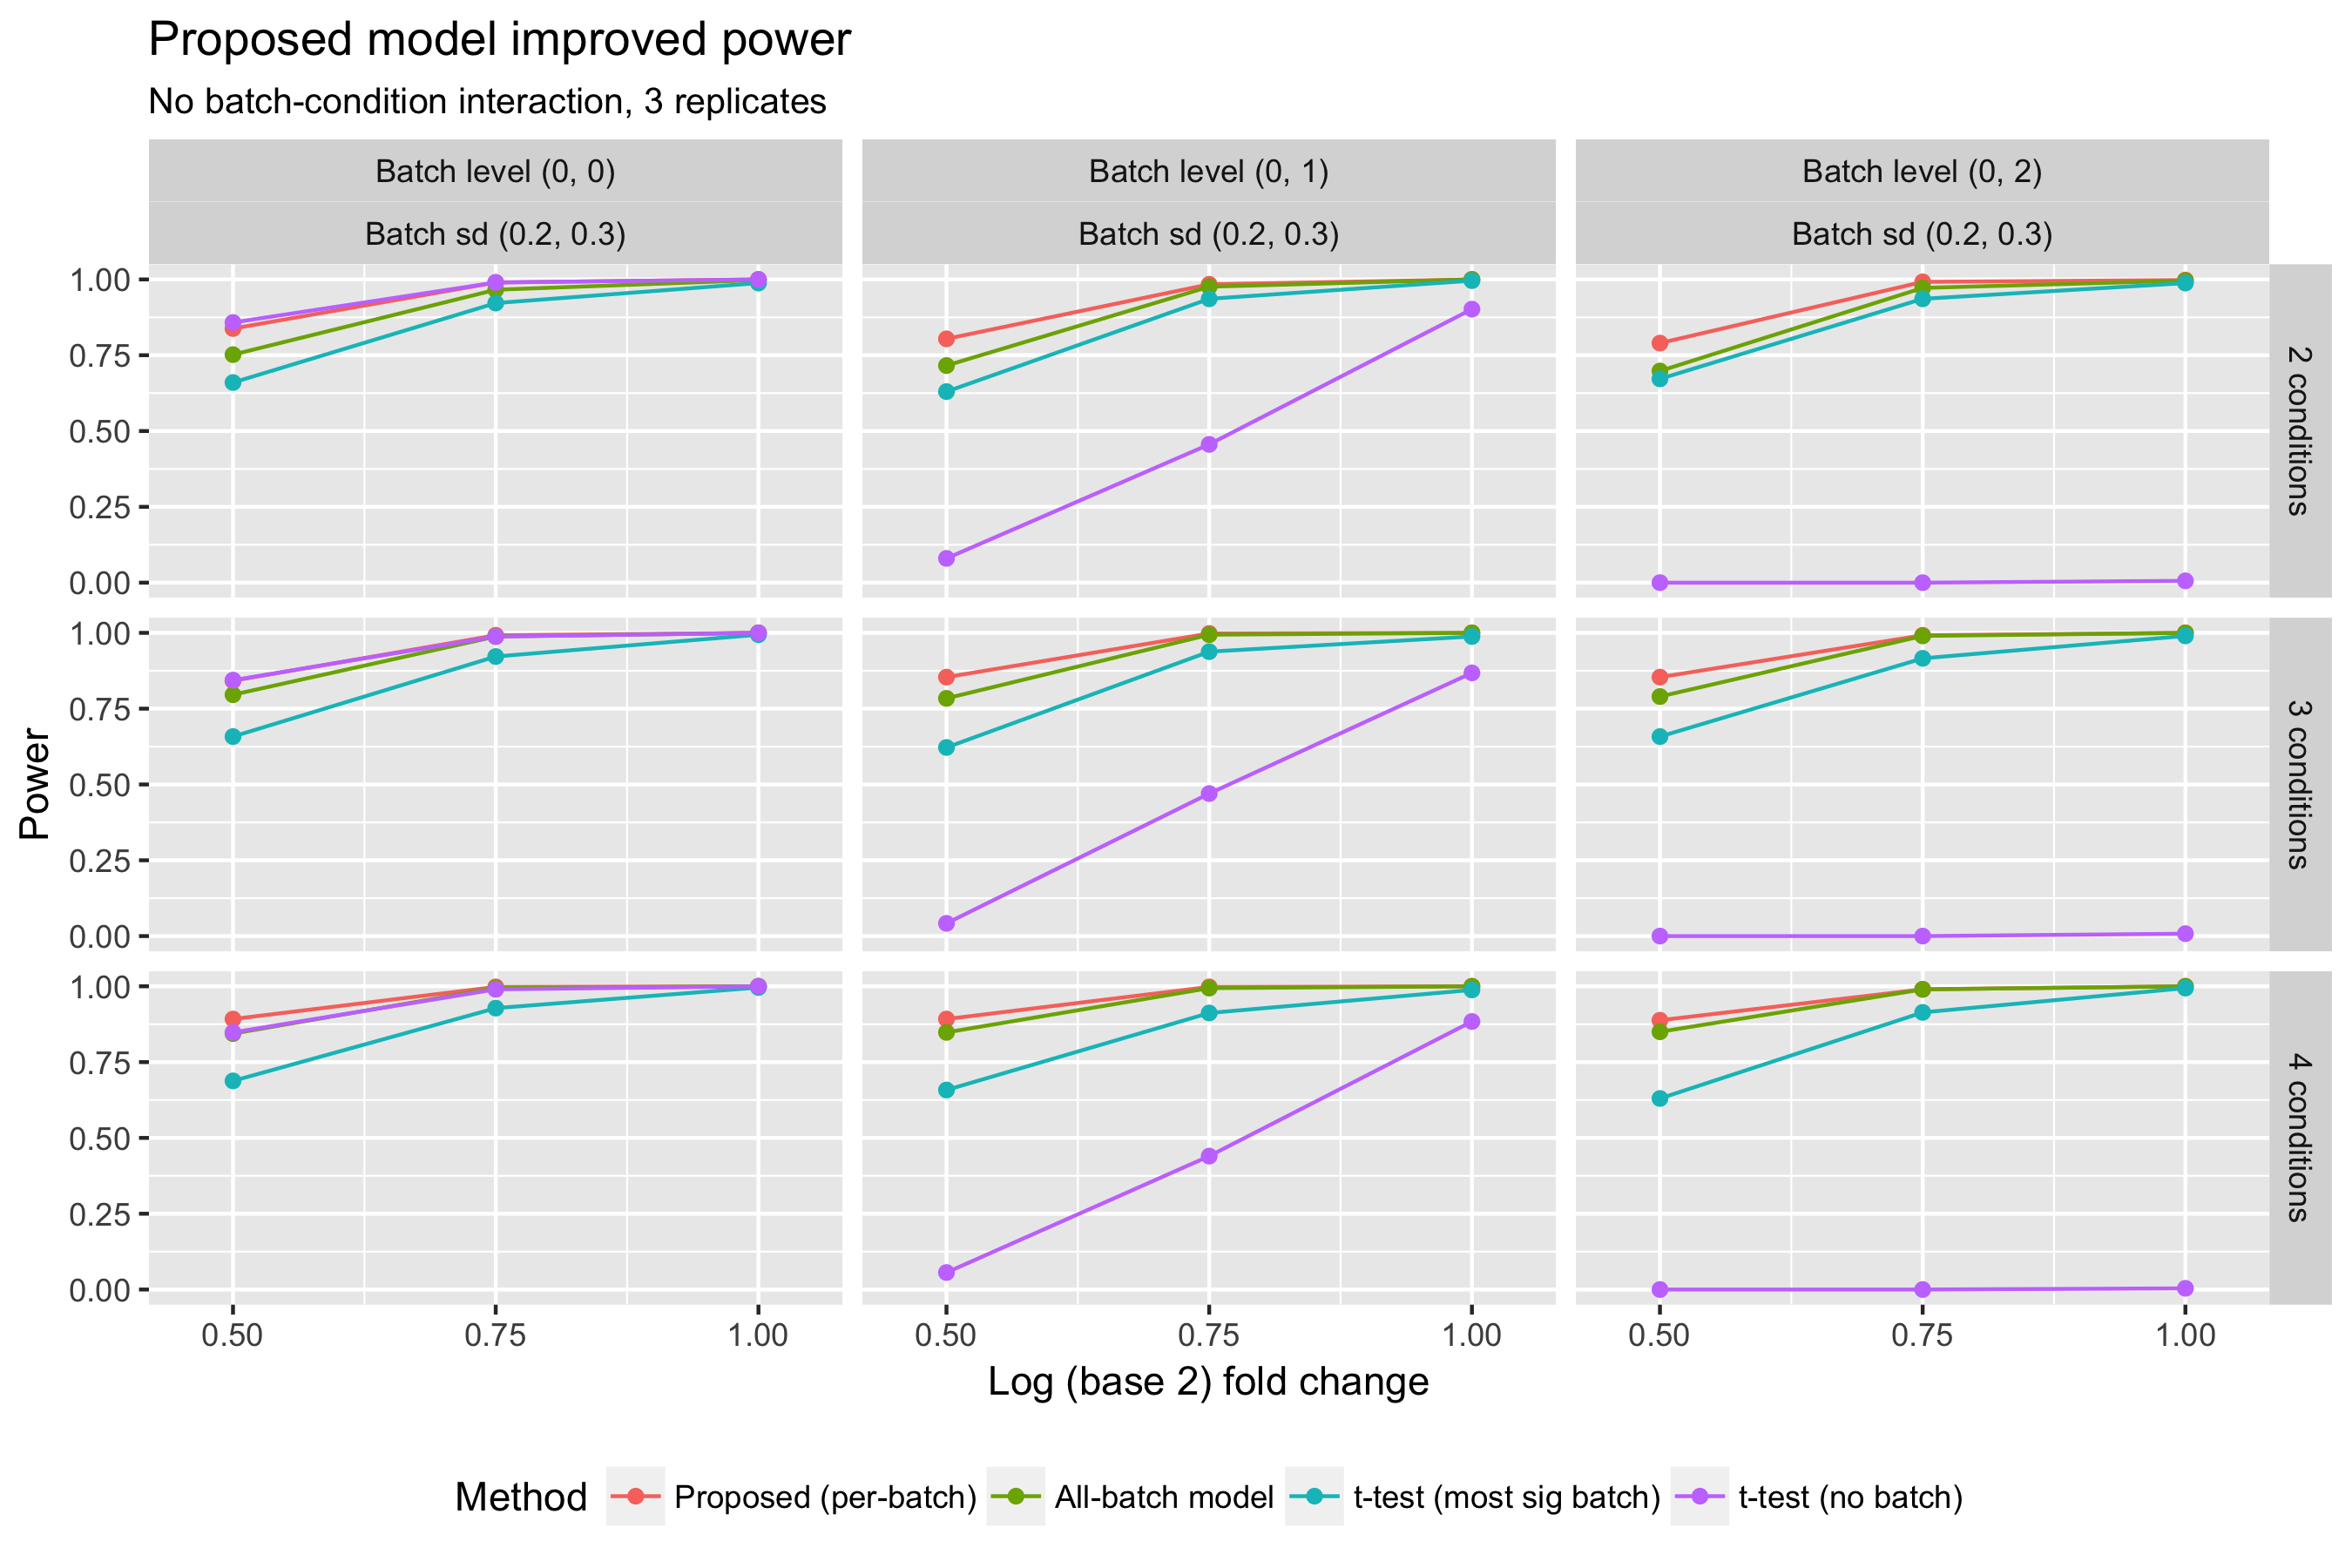
\includegraphics[width=.825\textwidth]{sim/synnull_pwr_3}
\caption{The proposed approach improved power with small sample sizes in almost all the scenarios, under various forms of batch effects including difference in intensity level (higher on the right) and difference in variability. Using $t$-test while ignoring batch effect gave similar performance in special cases with no difference in intensity level between batches, but its performance dramatically decreased in general cases. The proposed methods gave consistently improved performance compared with other methods by properly characterizing batch effects and leveraging all available information. Similar patterns were observed in other simulated scenarios with positive and negative interactions.\label{fig:synnull_pwr}}
\end{figure}

%\clearpage
%\begin{figure}[h!]
%\centering
%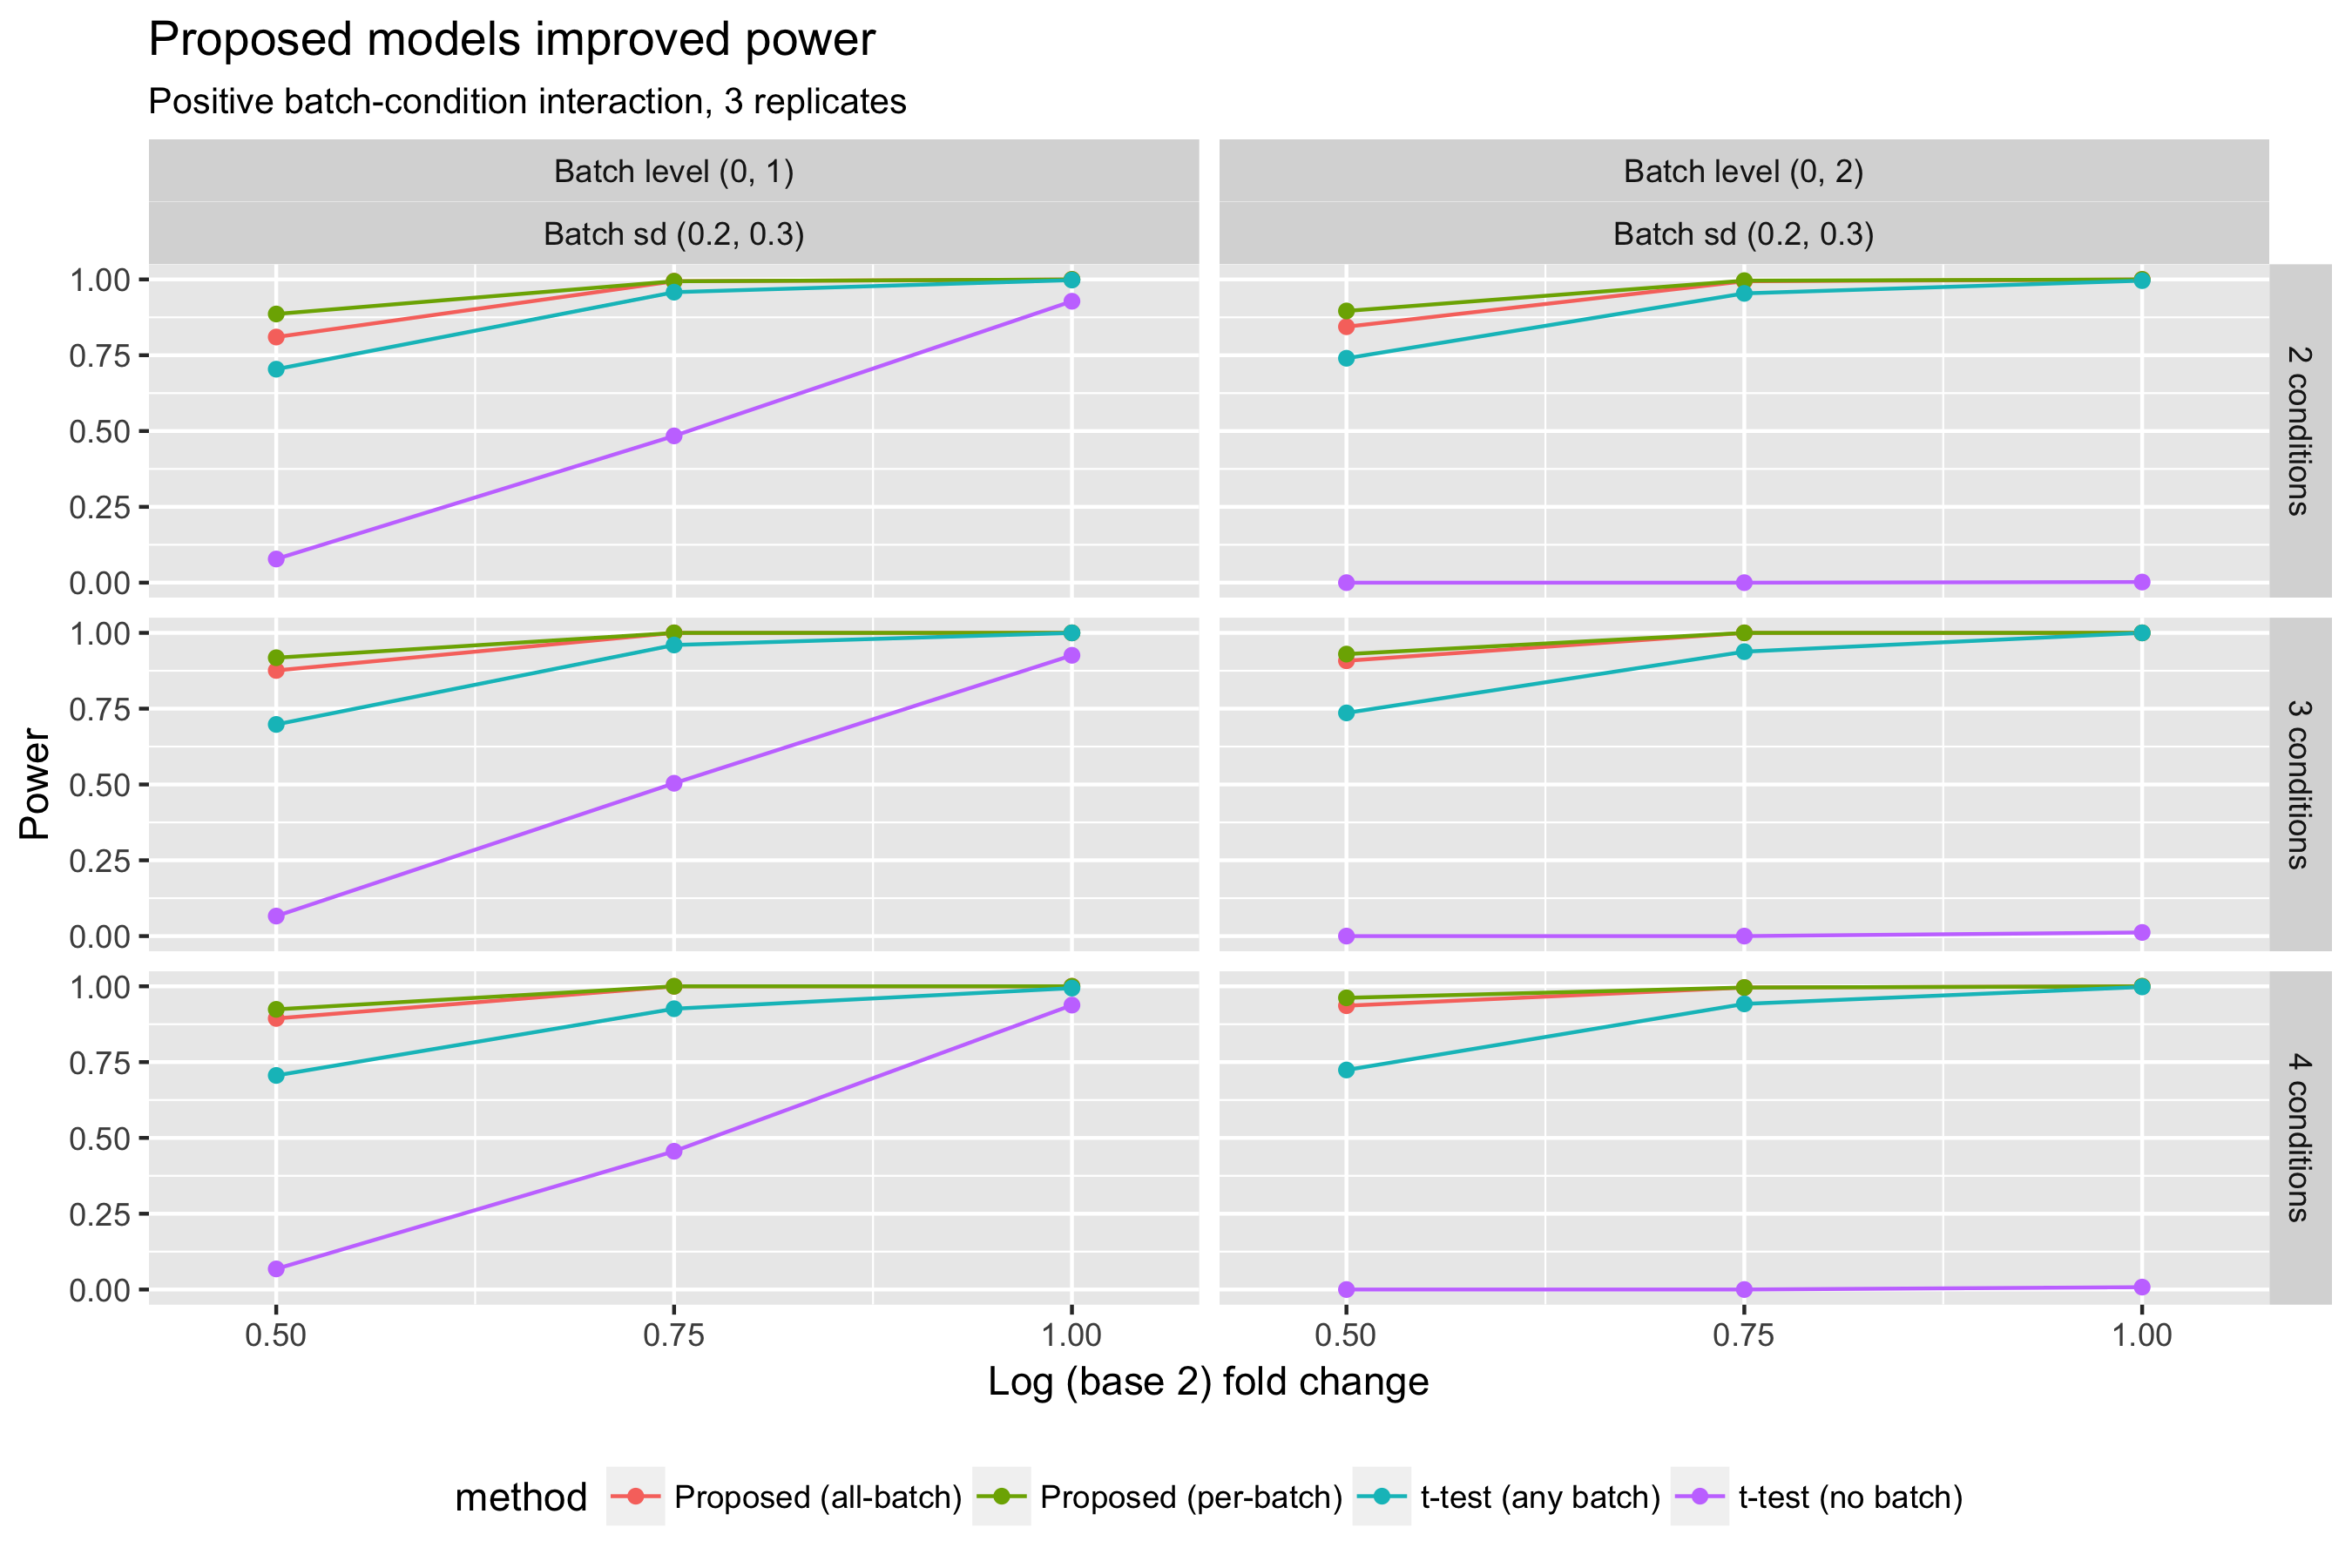
\includegraphics[width=.85\textwidth]{sim/synpos_pwr_3}\\
%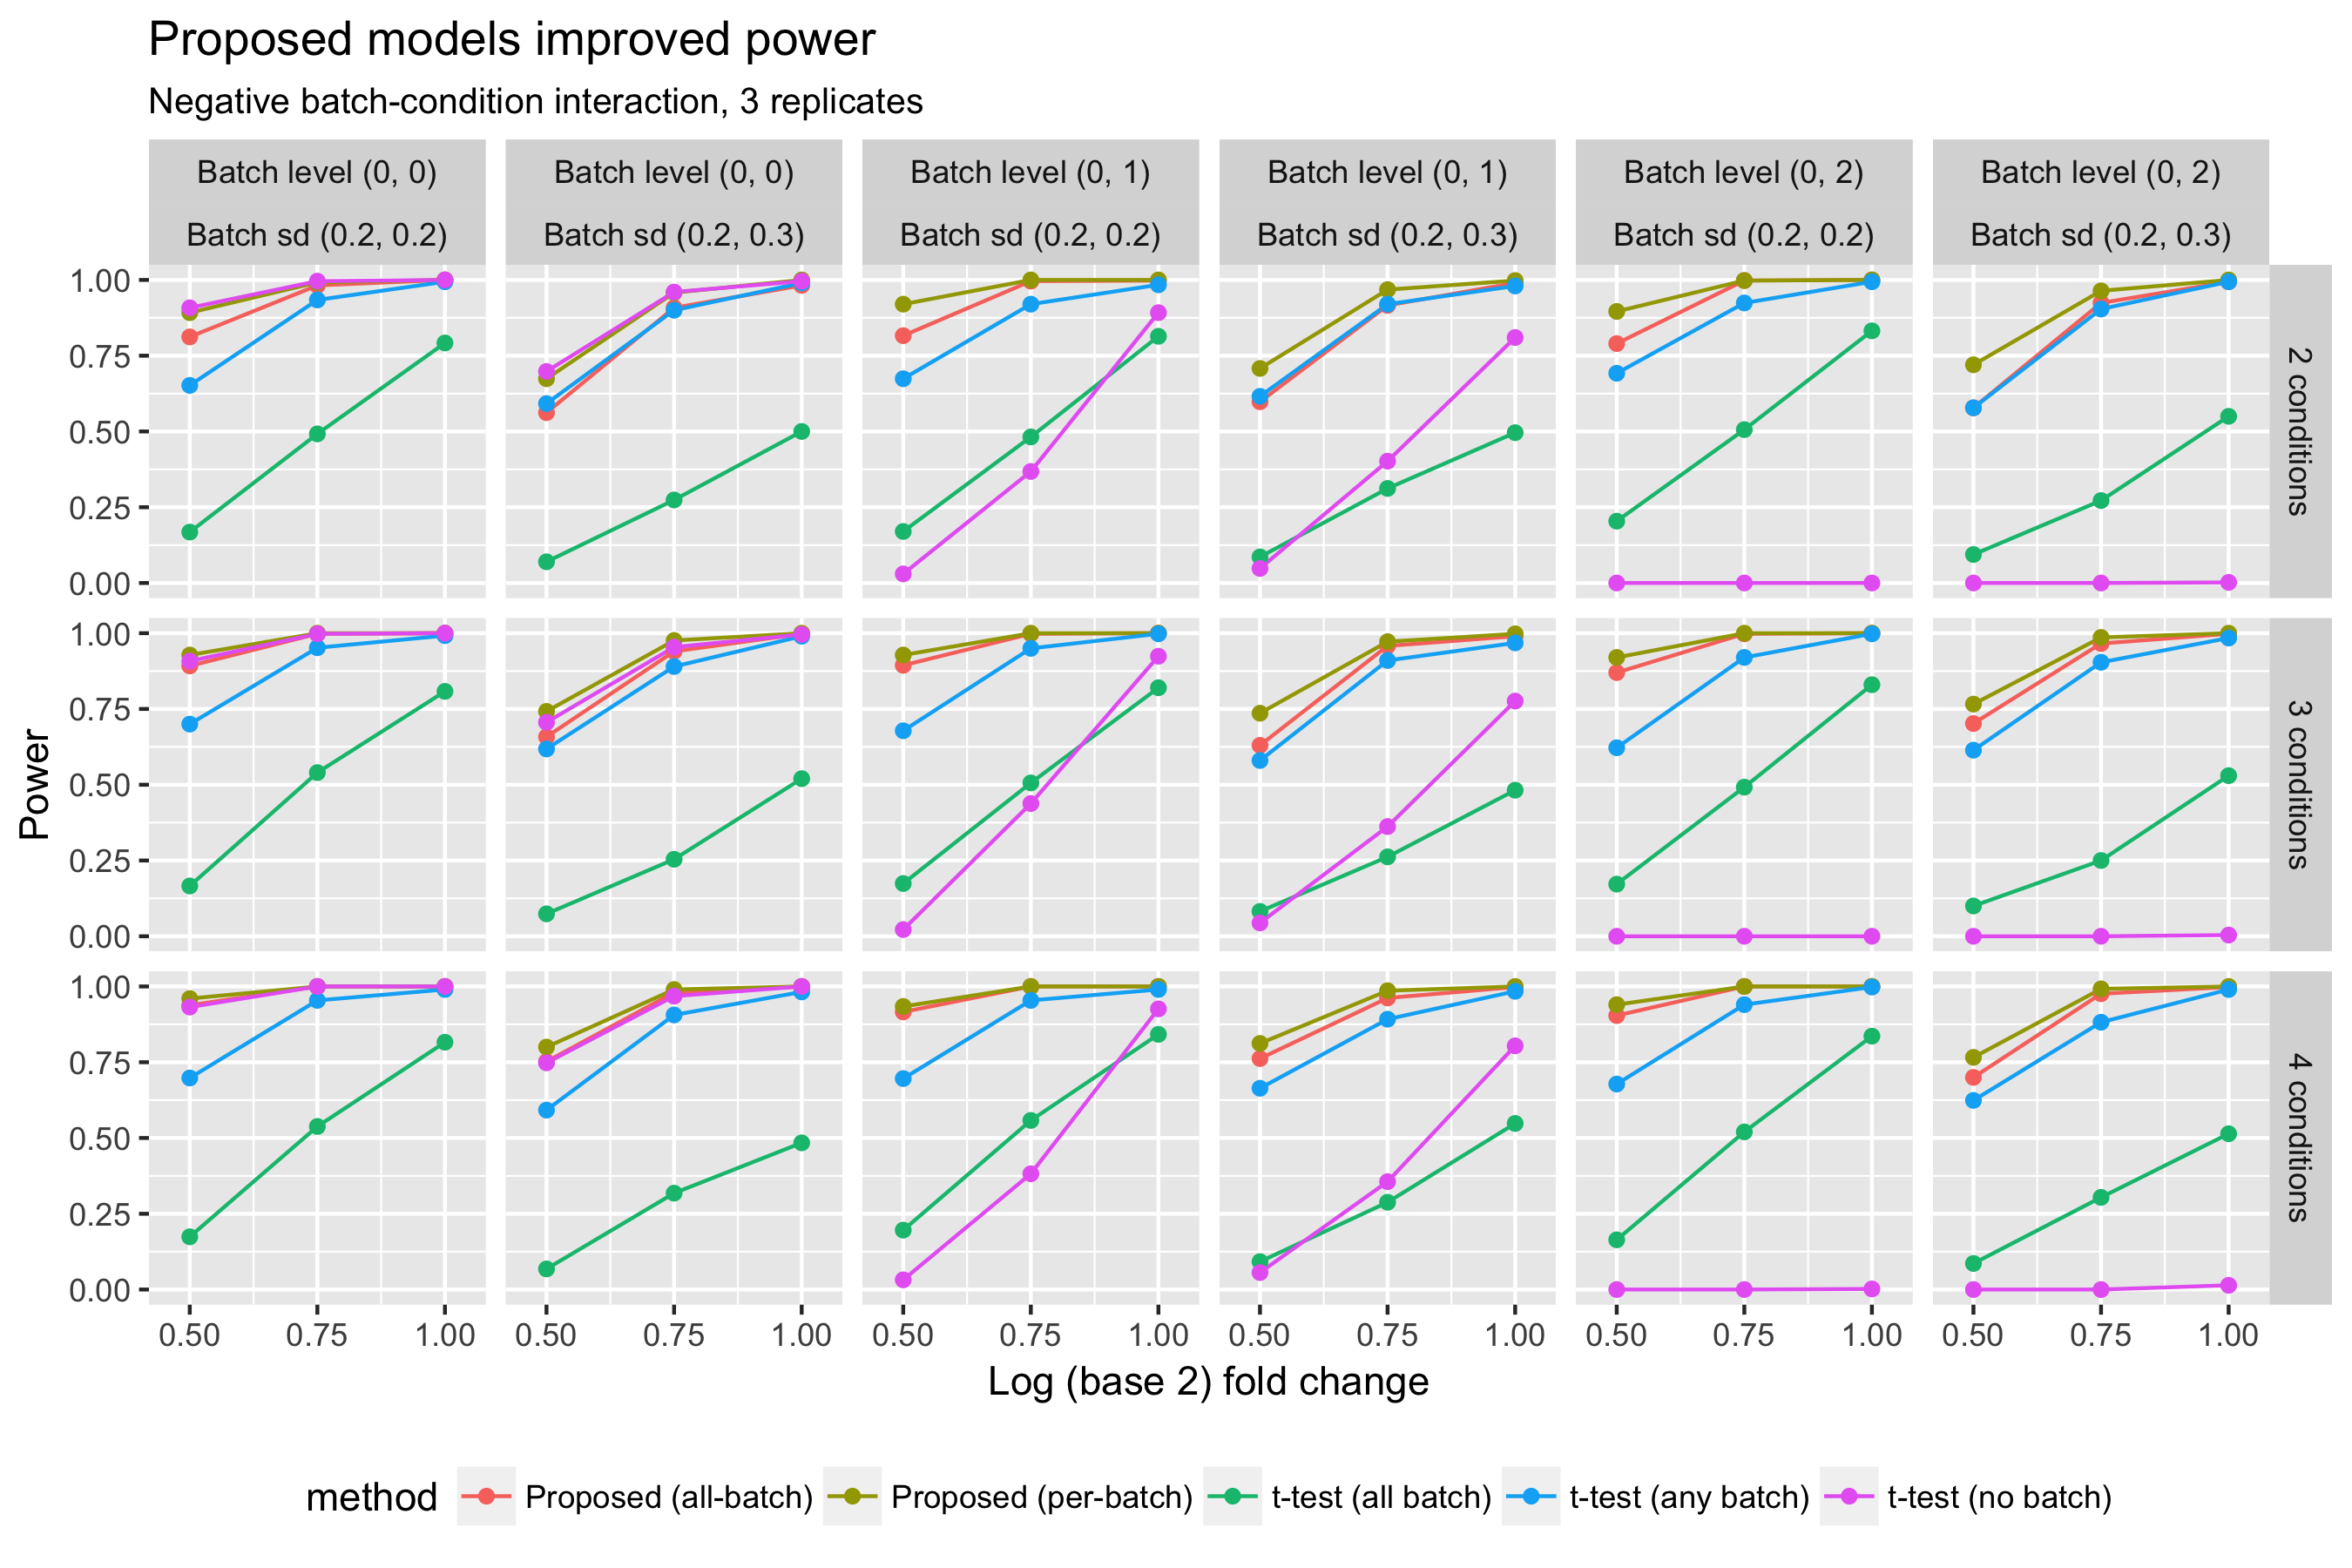
\includegraphics[width=.85\textwidth]{sim/synneg_pwr_3}
%\caption{With 3 replicates and under the scenarios with either positive or negative interaction, the proposed approach consistently improved power over other methods. Similar results were observed with 2 replicates. As in those cases with no interaction, the approaches using two-sample $t$-test did not benefit from data in additional conditions. Also, ignoring batch effects as applying $t$-test (no batch) lost power dramatically. \label{fig:syn_pwr_3}}
%\end{figure}

\begin{figure}[h!]
\centering
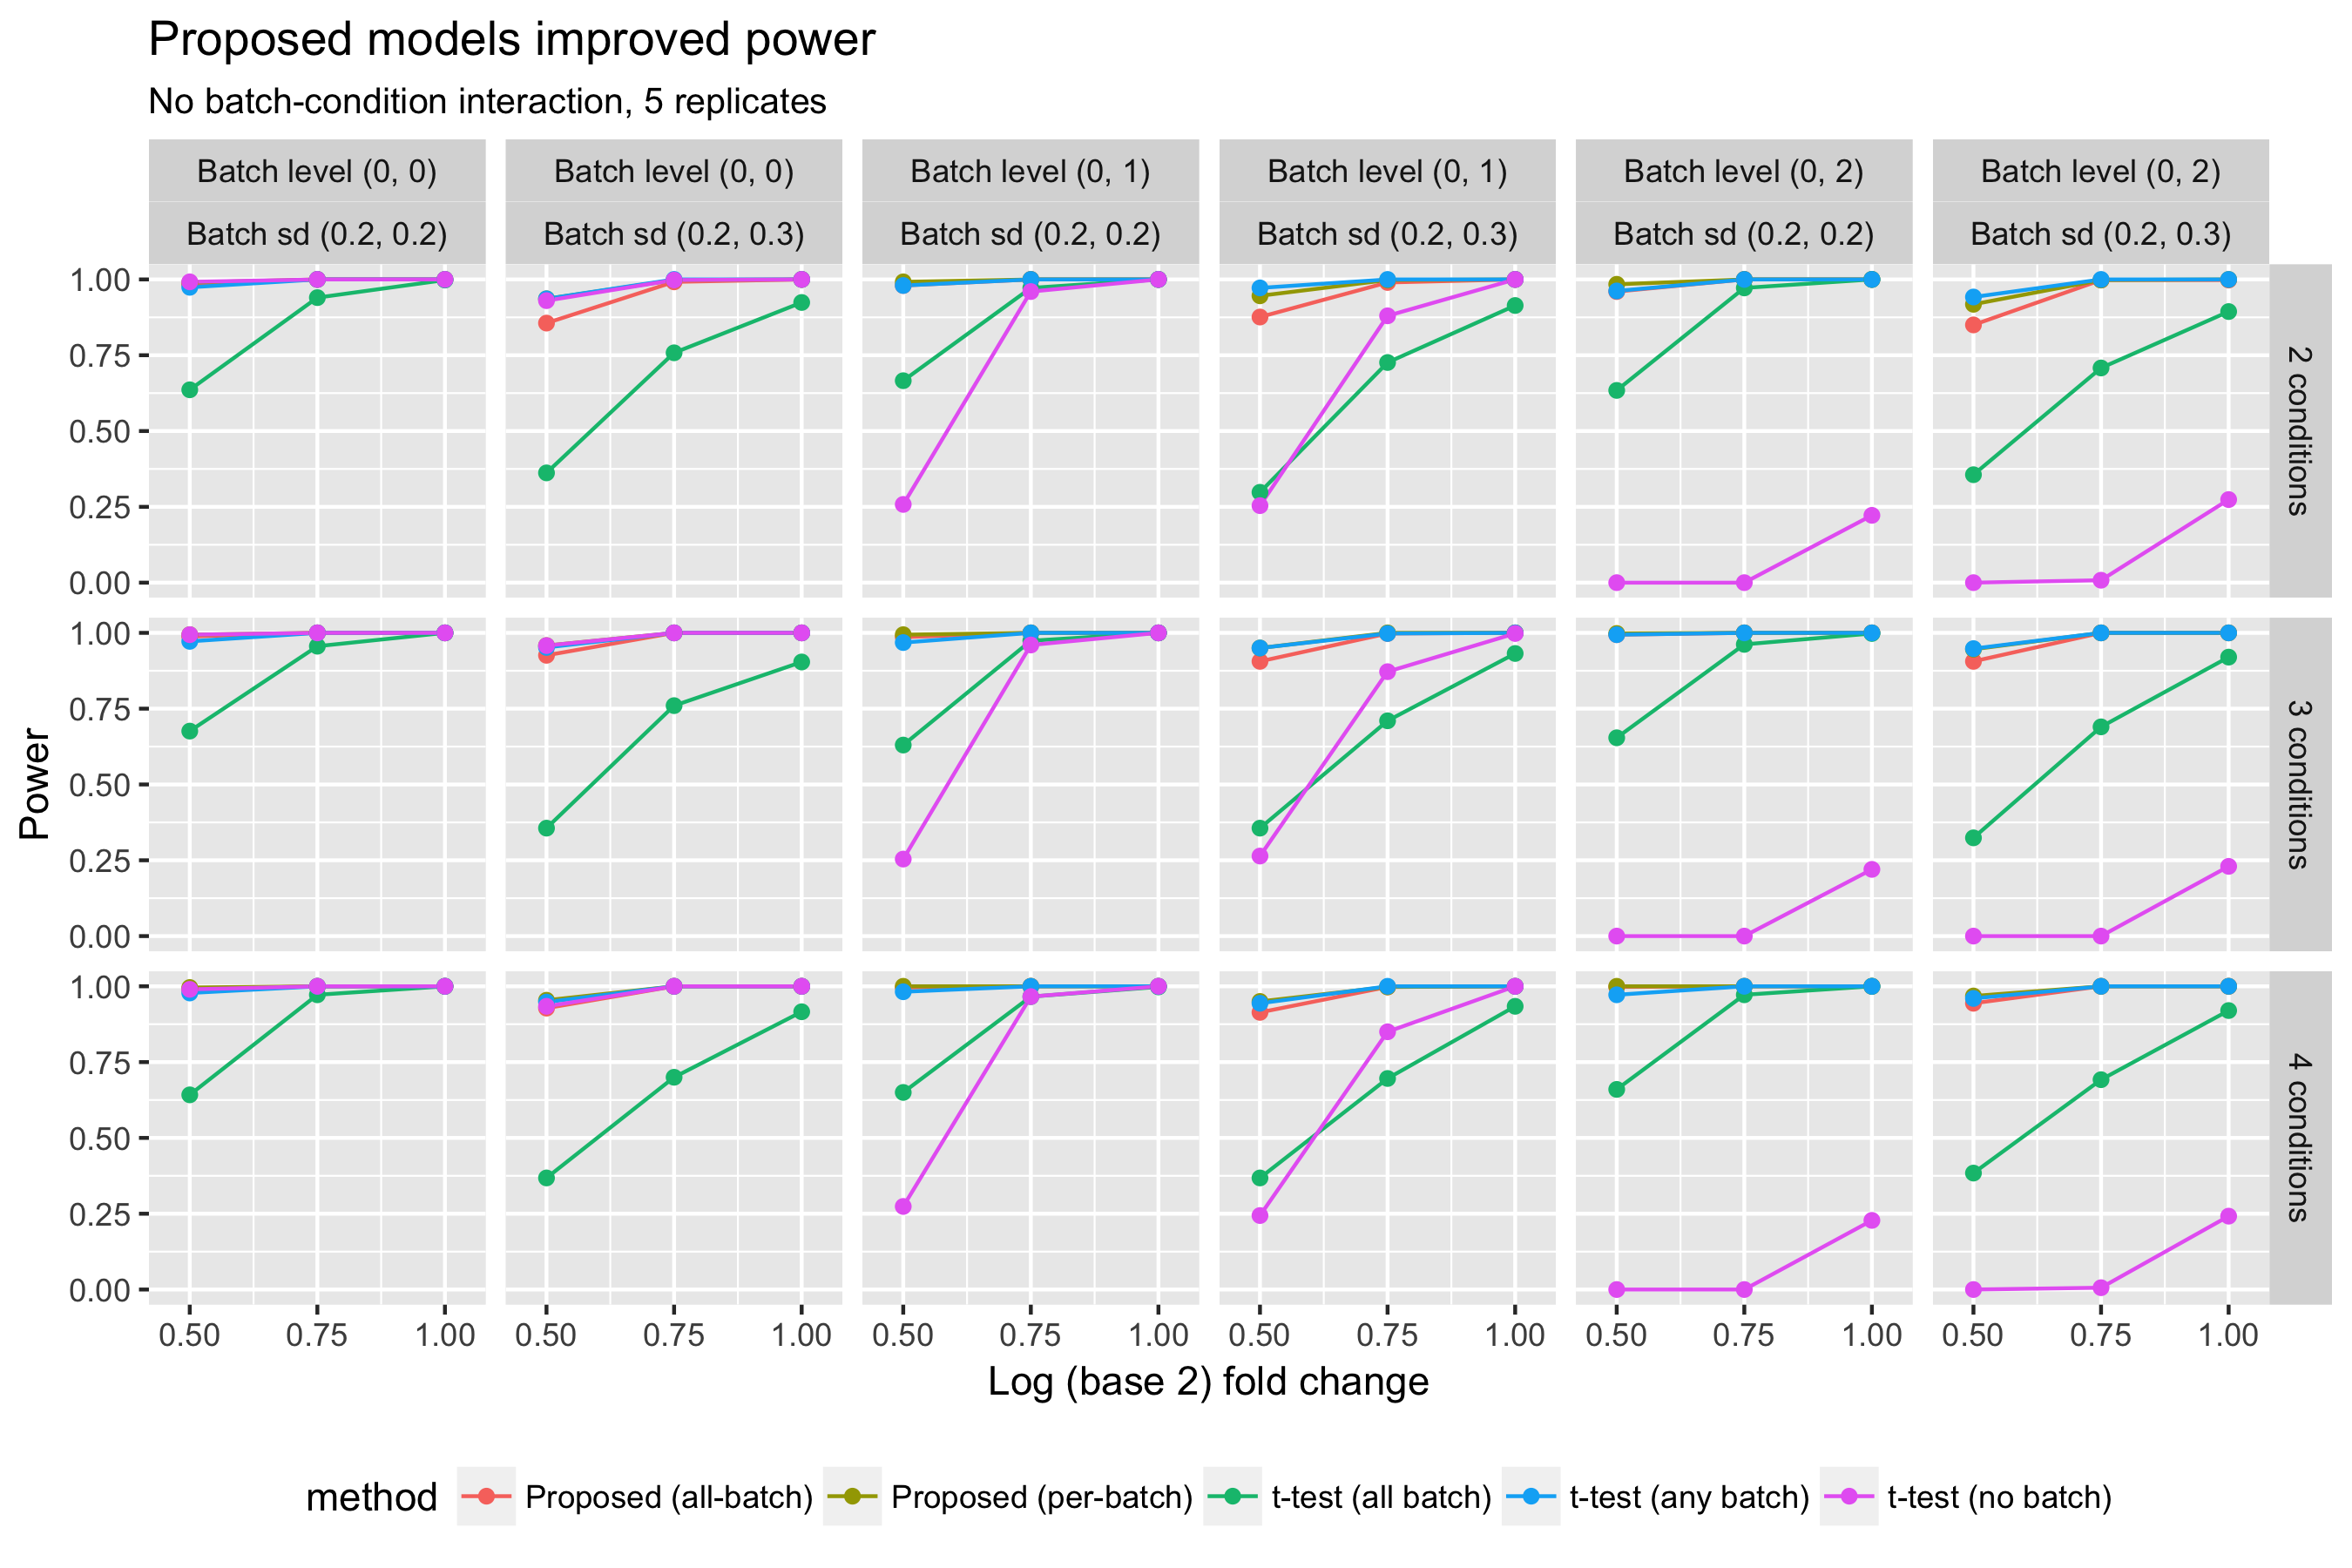
\includegraphics[width=.825\textwidth]{sim/synnull_pwr_5}
\caption{Ignoring batch effects lost power. The negative impact was only partially reduced by increasing the sample size to 5. Similar patterns were observed in other simulated scenarios. \label{fig:synnull_pwr_5}}
\end{figure}

\clearpage
%%%%%%%%%%%%%%%%%%%%%%%%%%%%%%%%%%%%%%%%%%%%%%%%%%%%%%%%%%%%%%%%
\subsection{TMT experiment}
\label{sec:tmtsim}

\todo{add the simulation for TMT experiment, batch vs plex?}


\clearpage
%%%%%%%%%%%%%%%%%%%%%%%%%%%%%%%%%%%%%%%%%%%%%%%%%%%%%%%%%%%%%%%%
\section{Sample size calculation and power analysis}

The proposed approach adjusts for the underlying protein abundance in the PTM significance analysis, which corrects the confounding factor with a cost of increased uncertainty. \todo{uncertainty? means variation?} We compared the required sample size with or without the adjustment to highlight the property (\sfigref{fig:size_prot}), based on a design of two conditions, in consideration of three pairs of standard deviations of log-intensities for modified and unmodified peptides: (0.2, 0.1), (0.2, 0.2), and (0.2, 0.4). 
%We considered a design with two conditions, where standard deviations of log-intensities of both modified and unmodified peptides were both set as $0.2$. 
We then characterized the advantage of general statistical modeling in complex designs in terms of sample size calculation (\sfigref{fig:size_grp}) and power analysis (\sfigref{fig:pwr_grp}). 

\begin{figure}[h!]
\centering
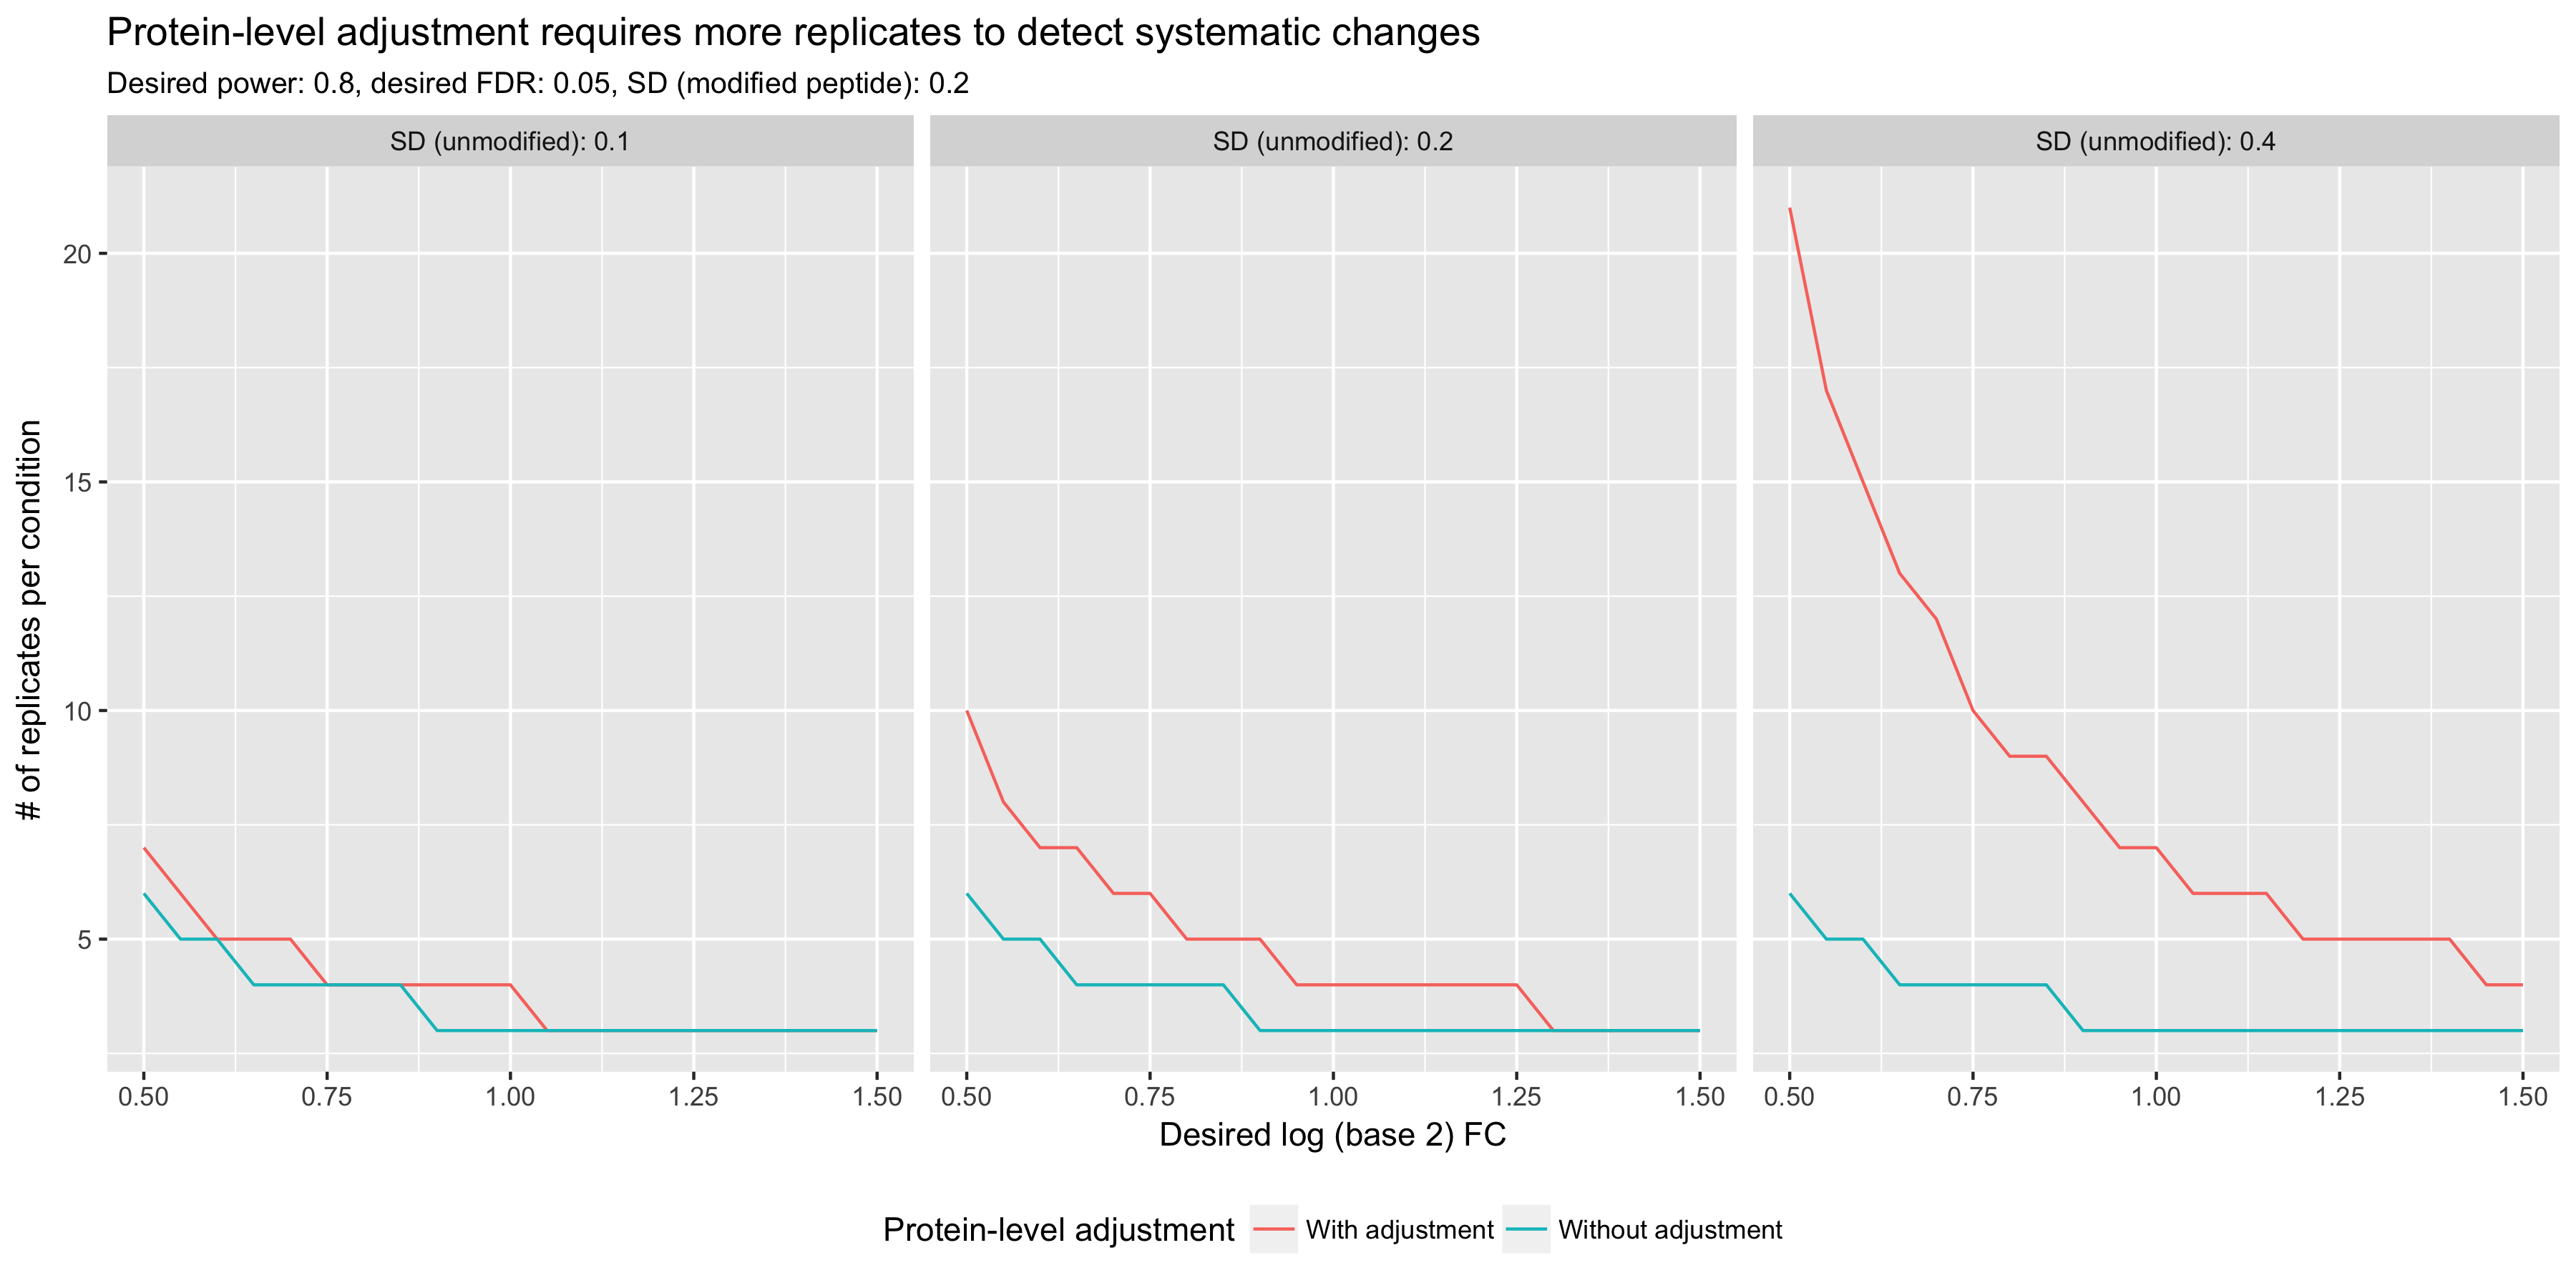
\includegraphics[width=\textwidth]{sim/size_prot}
\caption{Protein-level adjustment relies on the inference of protein abundance, which introduces additional uncertainty in the estimate of PTM difference. Therefore, the required sample size to detect a systematic change is higher than as expected for standard differential analysis without adjustment. The discrepancy can be profound if the uncertainty associated with the protein abundance estimate is greater than that of PTM abundance estimate. Sample size calculation without accounting for the uncertainty would lead to under-powered studies. \label{fig:size_prot}}
\end{figure}

\begin{figure}[h!]
\centering
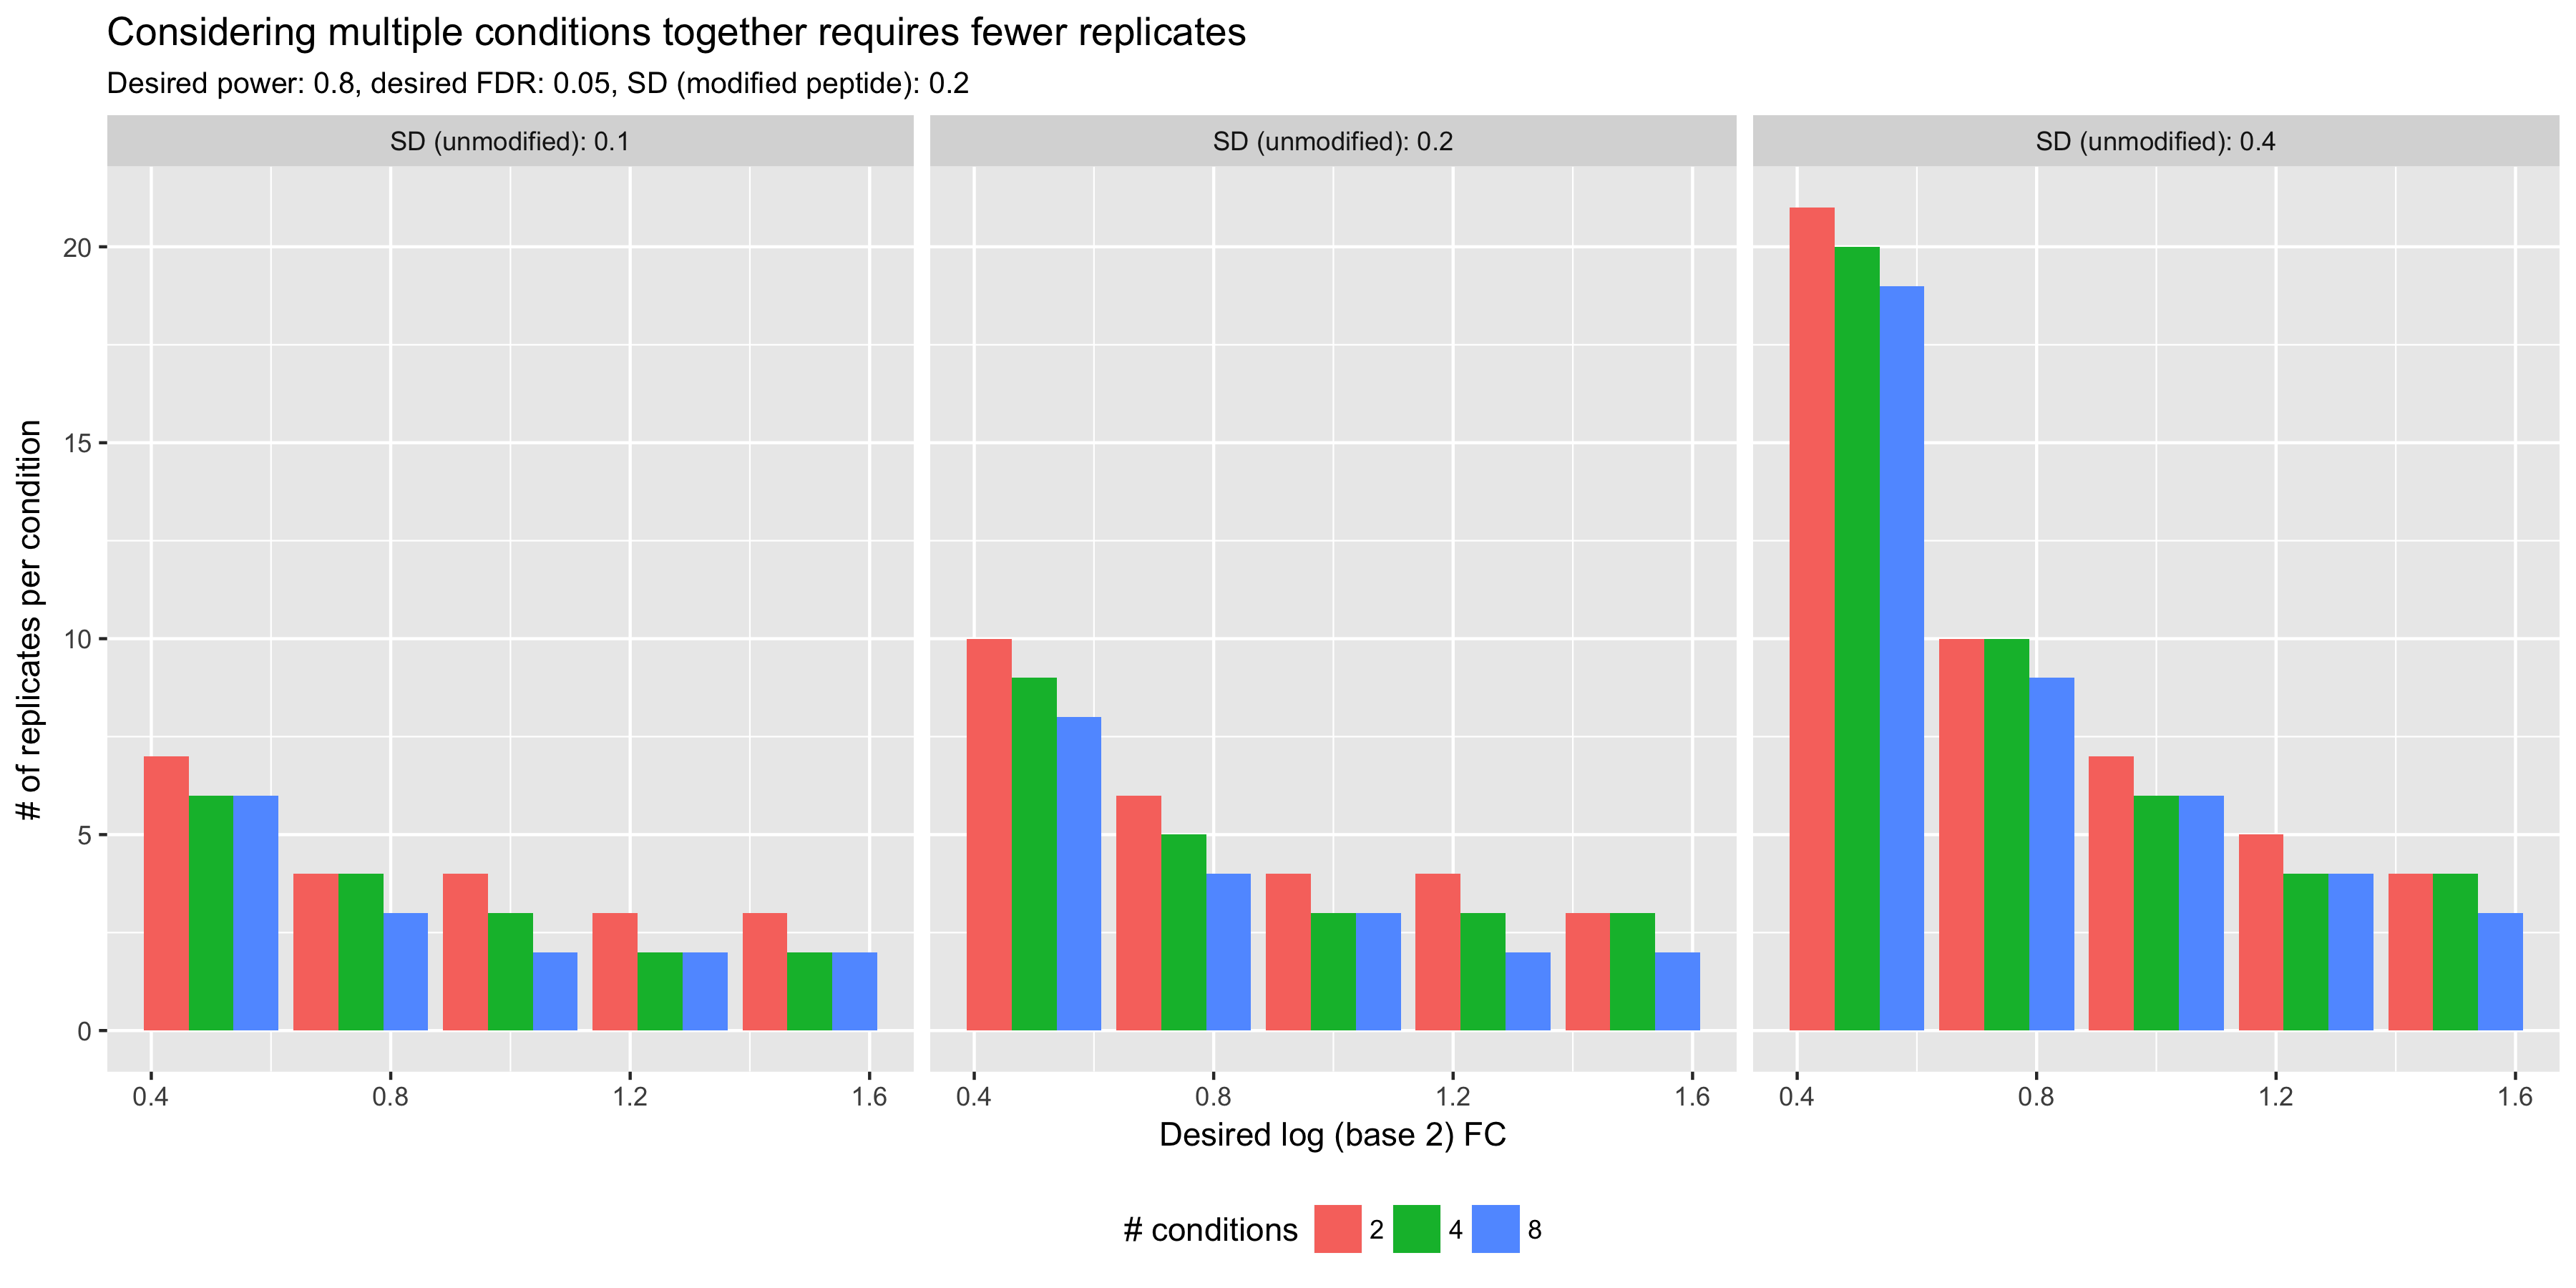
\includegraphics[width=\textwidth]{sim/size_grp}
%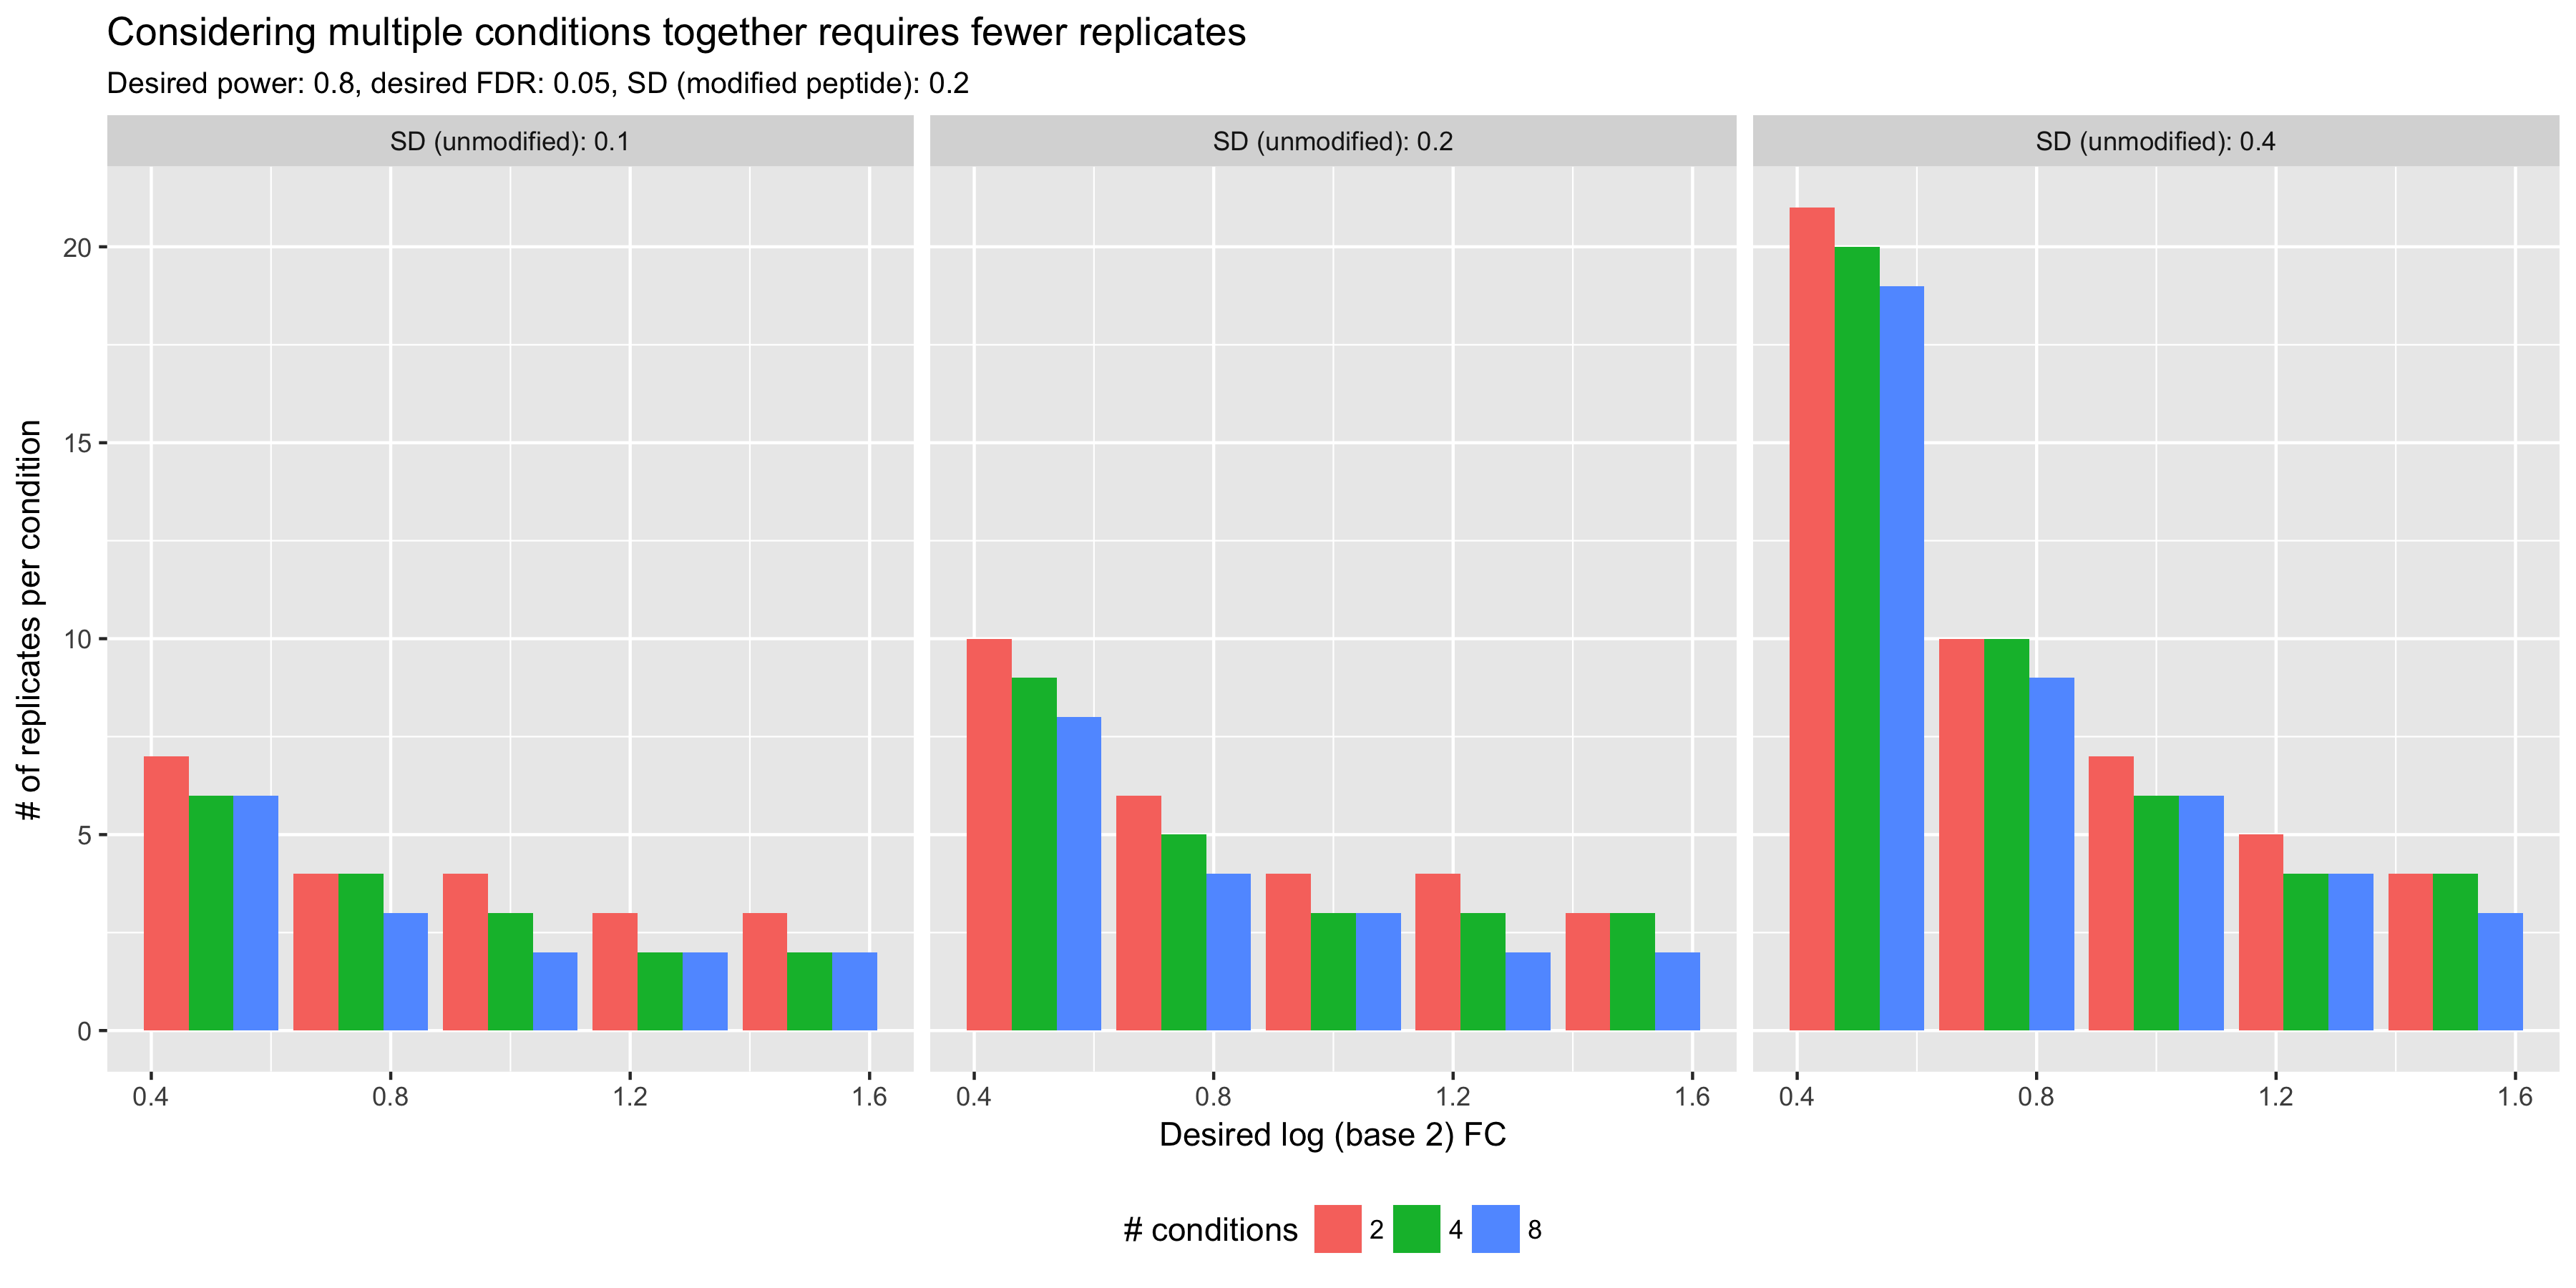
\includegraphics[width=.725\textwidth]{sim/size_grp}
\caption{In complex designs, simultaneously analyzing all the conditions effectively increases the degrees of freedom and requires fewer replicates. \label{fig:size_grp}}
\end{figure}

\begin{figure}[h!]
\centering
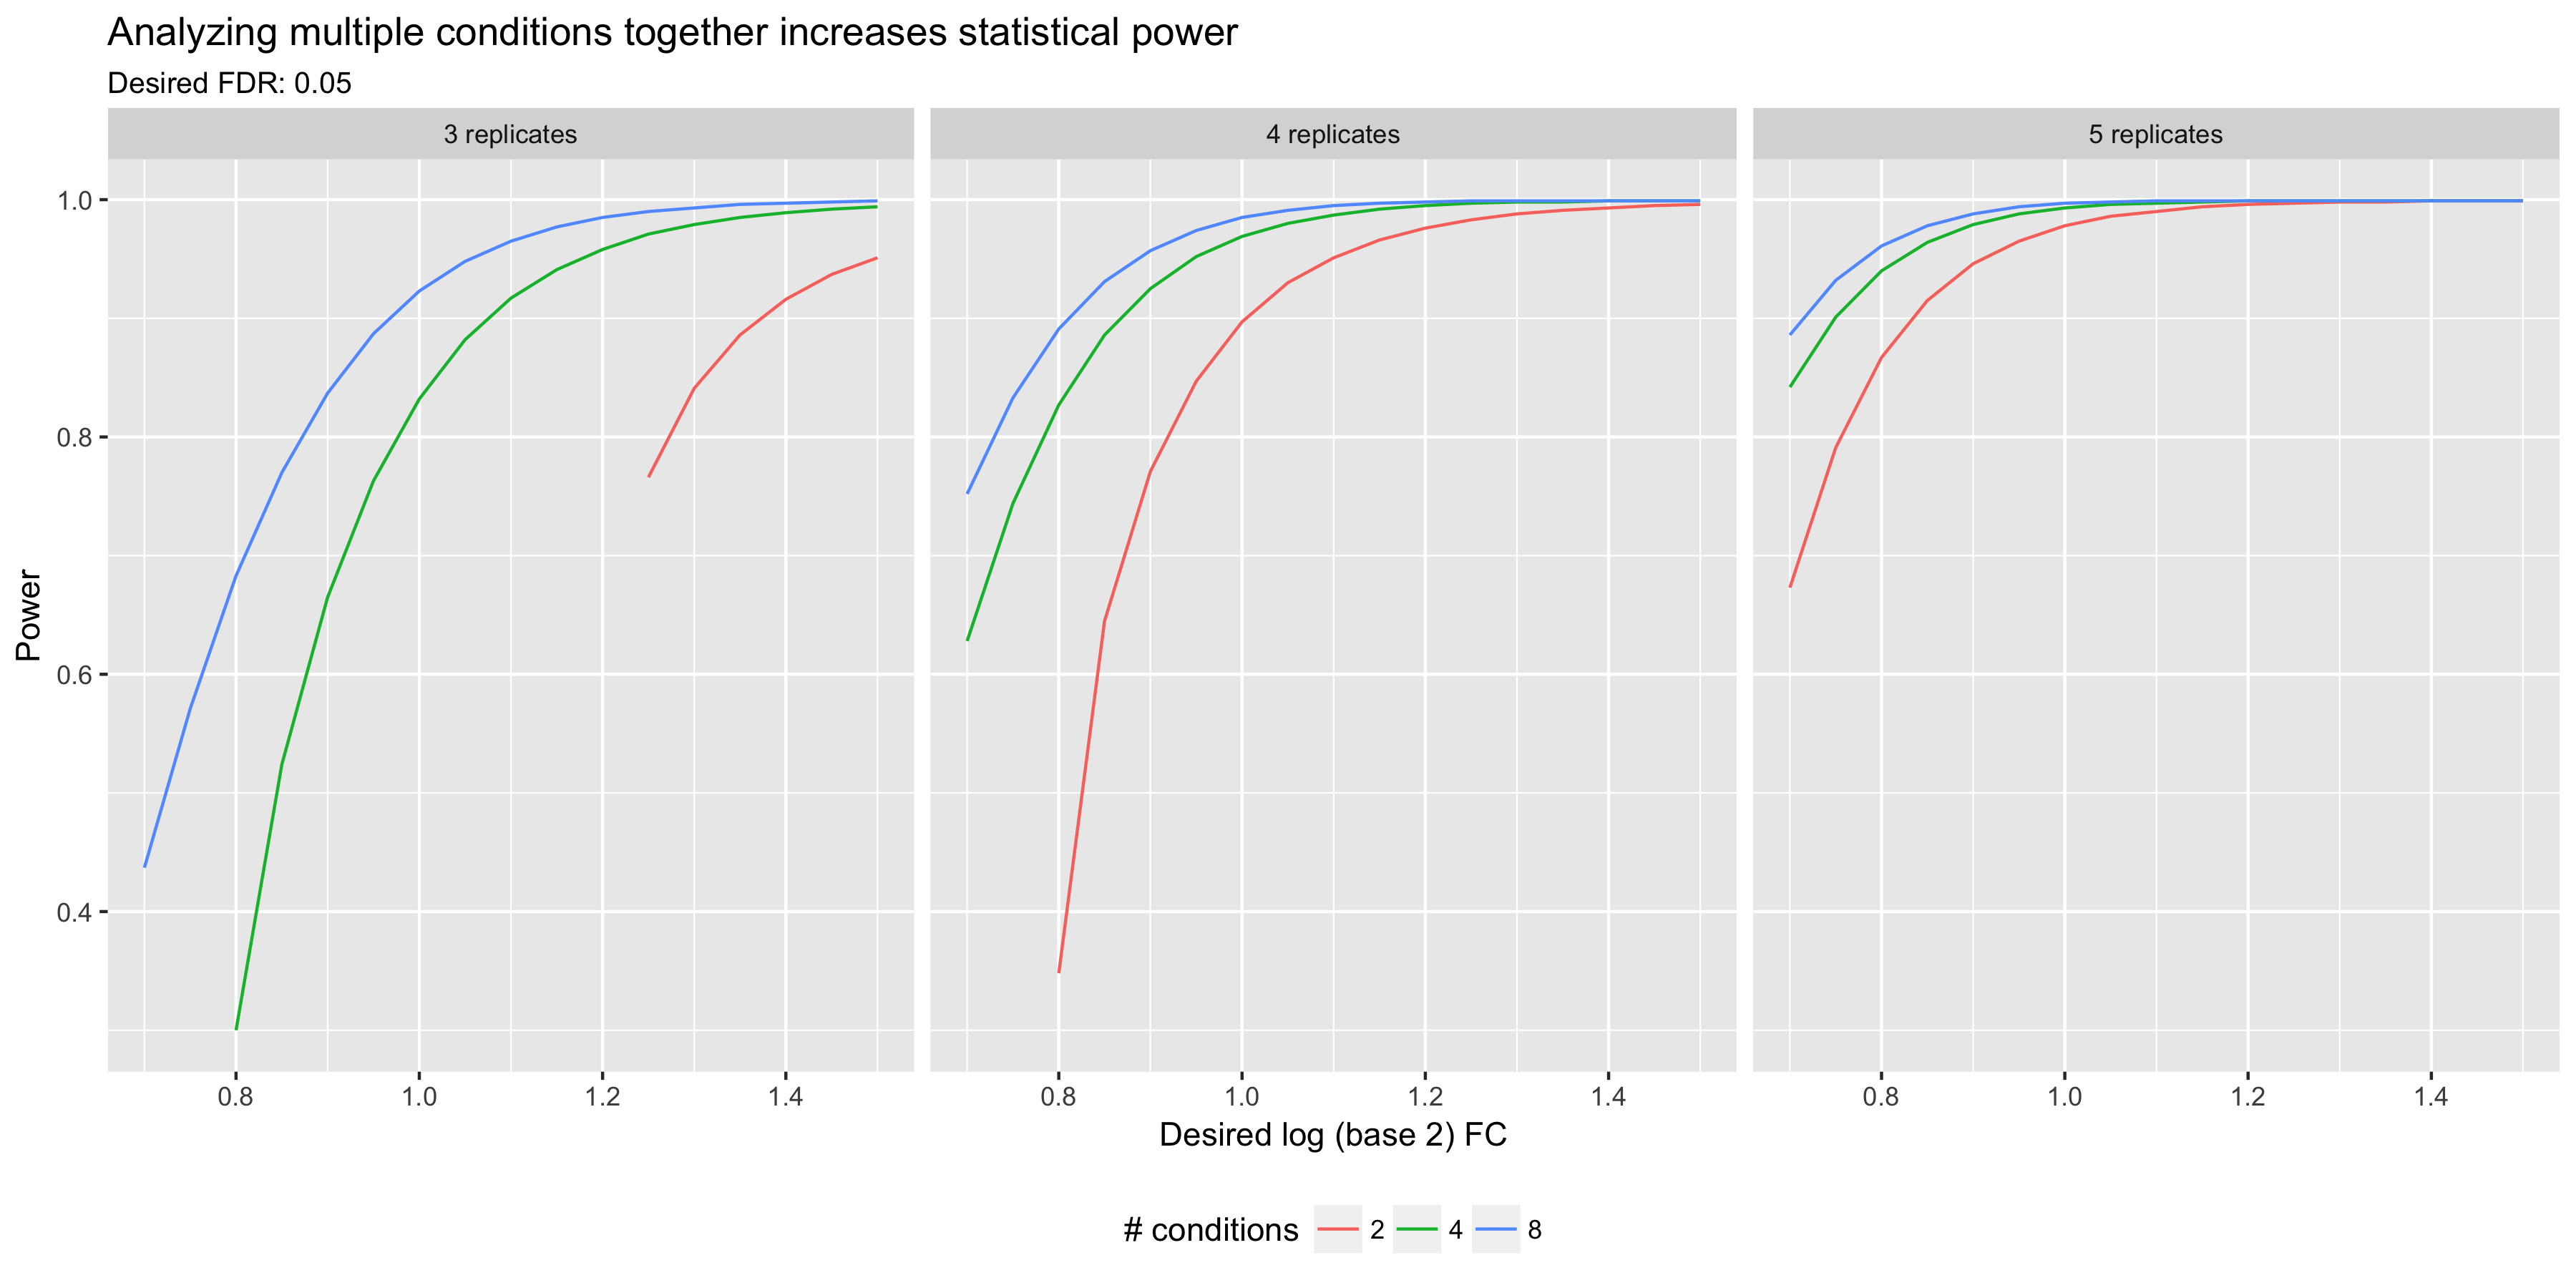
\includegraphics[width=\textwidth]{sim/pwr_grp}
%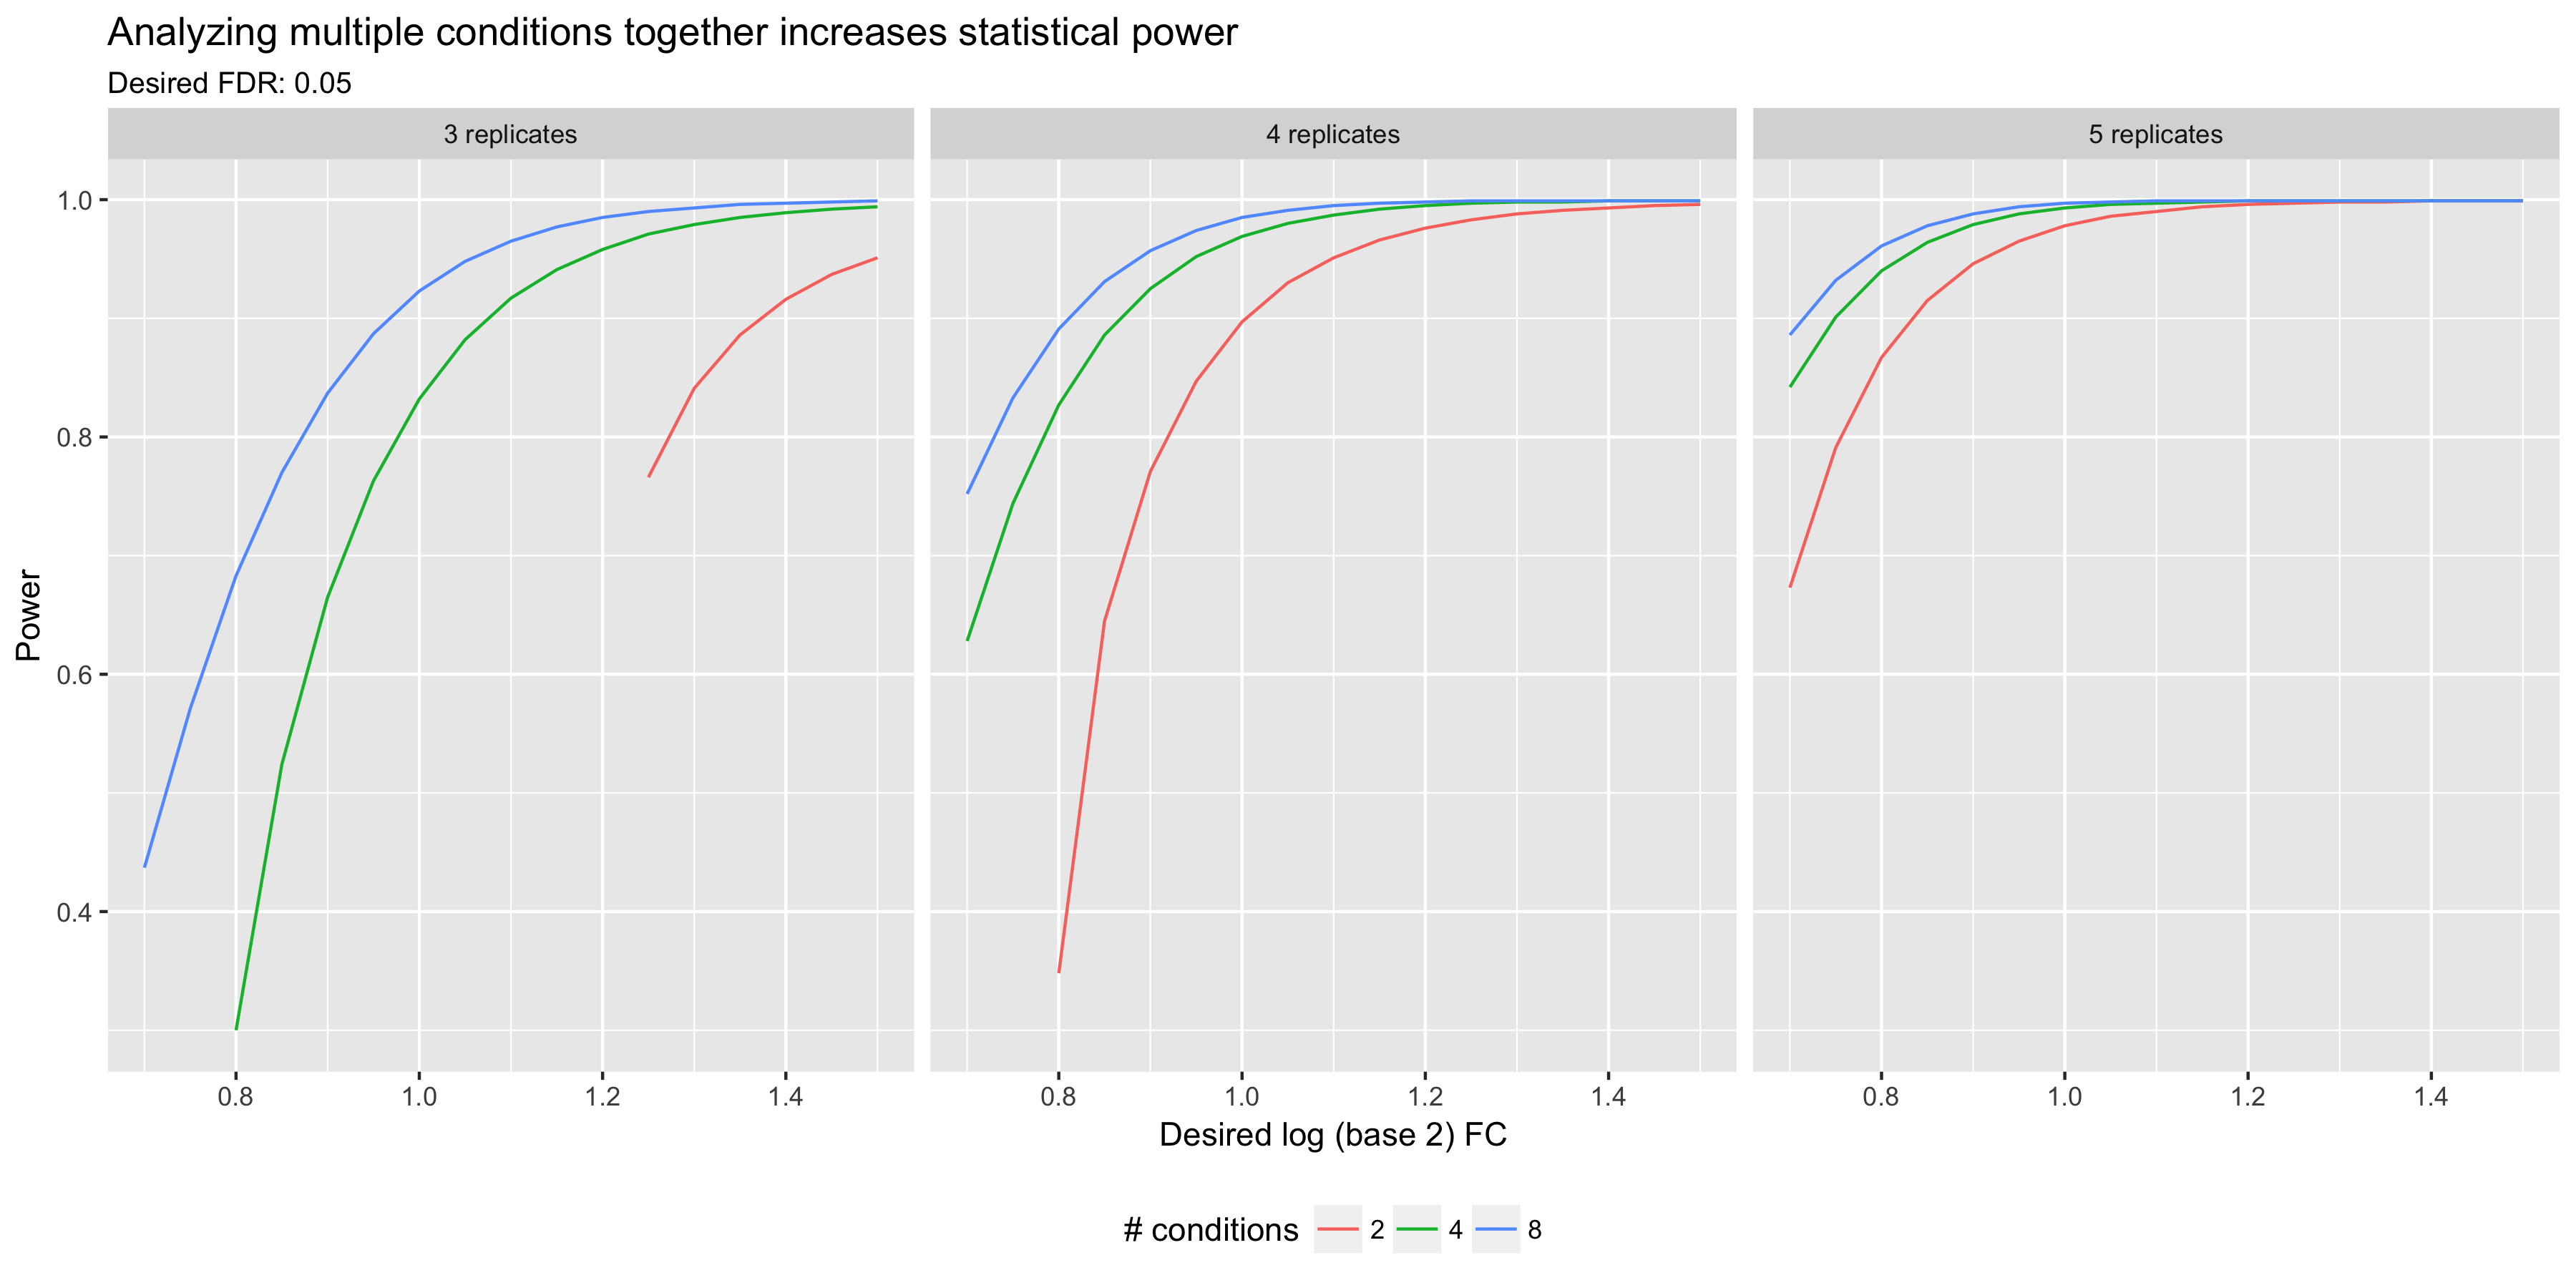
\includegraphics[width=.725\textwidth]{sim/pwr_grp}
\caption{Statistical power can be improved by increasing the sample size and analyzing multiple conditions together. \label{fig:pwr_grp}}
\end{figure}


\clearpage
%%%%%%%%%%%%%%%%%%%%%%%%%%%%%%%%%%%%%%%%%%%%%%%%%%%%%%%%%%%%%%%%
\section{Datasets : Biological investigation}

\todo{description and results}

%%%%%%%%%%%%%%%%%%%%%%%%%%%%%%%%%%%%%%%%%%%%%%%%%%%%%%%%%%%%%%%%
\clearpage
\section*{References}

\bibliographystyle{plain}
\bibliography{ptm_ref}

\end{document} 